\documentclass[12pt, a4paper]{article}
\usepackage[utf8]{inputenc}
%\usepackage[T1]{fontenc}
\usepackage[ngerman]{babel}
\usepackage{babel}
\usepackage{amsmath, amssymb, amsthm}
\usepackage{geometry}
\usepackage{graphicx}
\usepackage[hidelinks]{hyperref}
\usepackage{pgfplots}
\pgfplotsset{compat=1.18}
\usepackage{tikz}
\usepackage{float}
\usepackage{booktabs}
\usepackage{enumitem}
\usepackage{xcolor}
\usepackage{colortbl}
\usepackage{array}
\usepackage{multirow}
\usepackage{microtype}
\usepackage{enumitem}
\setlist[itemize,1]{label=-}

\hypersetup{
	colorlinks=true,
	linkcolor=blue!60!black,
	urlcolor=blue!60!black,
	citecolor=blue!60!black
}

\geometry{left=2.5cm, right=2.5cm, top=2.5cm, bottom=2.5cm}

\definecolor{tabblue}{RGB}{220,230,245}
\definecolor{tabgreen}{RGB}{220,245,225}
\definecolor{taborange}{RGB}{255,240,220}
\definecolor{tabgray}{RGB}{240,240,240}
\definecolor{headerblue}{RGB}{50,90,160}
\definecolor{proofbg}{RGB}{248,248,255}

\theoremstyle{definition}
\newtheorem{definition}{Definition}[section]
\newtheorem{satz}{Satz}[section]
\newtheorem{lemma}{Lemma}[section]
\newtheorem{korollar}{Korollar}[section]
\newtheorem{bemerkung}{Bemerkung}[section]
\newtheorem{beispiel}{Beispiel}[section]
\newtheorem{proposition}{Proposition}[section]

\newcolumntype{C}[1]{>{\centering\arraybackslash}m{#1}}
\newcolumntype{L}[1]{>{\arraybackslash}m{#1}}

\title{
	\textbf{Die Rotationsmethode zur Kurvendiskussion} \\
	\large Reduktion höherer Ableitungen auf die erste Ableitung \\
	durch geometrische Transformation des Funktionsgraphen \\[1ex]
	\normalsize mit Ausblick auf Anwendungen in der photonischen Transfermatrix-Theorie
}
\author{Stephan Epp}
\date{\today}

\begin{document}
	
	\maketitle
	\tableofcontents
	\newpage
	
	%%=====================================================================
	\section{Einleitung und Motivation}
	%%=====================================================================
	
	Die klassische Kurvendiskussion einer differenzierbaren Funktion $f$ erfordert
	die Berechnung mehrerer Ableitungen: Die \emph{erste} Ableitung $f'$ liefert
	Informationen über Monotonie und lokale Extrema, die \emph{zweite} Ableitung
	$f''$ klärt Krümmungsverhalten und Wendepunkte, und höhere Ableitungen
	erlauben die Klassifikation von Sattelpunkten sowie die Bestimmung der
	Krümmungsrichtung in Sonderfällen.
	
	Diese Arbeit stellt eine geometrische Beobachtung vor, die es ermöglicht,
	\emph{die gesamte Kurvendiskussion -- einschließlich der Wendepunktbestimmung
		-- allein auf die erste Ableitung zurückzuführen}, indem der Graph der
	Funktion (oder die Funktion selbst) geeignet rotiert wird. Wendepunkte des
	ursprünglichen Graphen werden dabei zu Extrema des rotierten Graphen
	transformiert und können somit mittels des Kriteriums für lokale Extrema,
	d.\,h.\ durch die erste Ableitung, identifiziert werden.
	
	Der Ansatz ist nicht nur methodisch ökonomisch, sondern wirft auch
	grundsätzliche Fragen über die geometrische Invarianz analytischer
	Eigenschaften von Kurven auf. Als praktisches Werkzeug wird die
	\emph{Winkel-Sortier-Tabelle} (WST) eingeführt, die alle analytisch
	relevanten Punkte nach ihrem erforderlichen Rotationswinkel ordnet und
	so eine vollständige Kurvendiskussion mit einer einzigen, schrittweise
	durchgeführten Drehbewegung des Graphen ermöglicht.
	
	Im abschliessenden Ausblick (Abschnitt~\ref{sec:ausblick}) wird gezeigt,
	dass strukturell eng verwandte Ideen in der modernen Nanooptik und
	Quantenmechanik -- insbesondere in der Transfermatrix-Theorie photonischer
	Schichtsysteme -- wiederkehren und die Rotationsmethode dort eine
	überraschend präzise Entsprechung findet.
	
	%%=====================================================================
	\section{Mathematische Grundlagen}
	%%=====================================================================
	
	\subsection{Klassische Kurvendiskussion}
	
	Sei $f: D \subseteq \mathbb{R} \to \mathbb{R}$ eine hinreichend oft
	differenzierbare Funktion. Die klassische Kurvendiskussion analysiert:
	
	\begin{enumerate}[label=\arabic*.]
		\item \textbf{Nullstellen:} $f(x) = 0$
		\item \textbf{Monotonie und Extrema:} Analyse von $f'$
		\item \textbf{Krümmung und Wendepunkte:} Analyse von $f''$
		\item \textbf{Höhere Eigenschaften:} Analyse von $f'''$, $f^{(4)}$, \ldots
	\end{enumerate}
	
	\begin{definition}[Lokales Extremum]
		Ein Punkt $x_0 \in D$ heißt \emph{lokales Maximum} (bzw.\ \emph{Minimum})
		von $f$, falls eine Umgebung $U(x_0)$ existiert mit
		$f(x) \leq f(x_0)$ (bzw.\ $f(x) \geq f(x_0)$) für alle $x \in U(x_0)$.
		Ein lokales Extremum heißt \emph{strikt}, wenn die Ungleichung für
		$x \neq x_0$ strikt gilt.
	\end{definition}
	
	\begin{definition}[Wendepunkt]
		Ein Punkt $x_0 \in D$ heißt \emph{Wendepunkt} von $f$, falls $f''(x_0) = 0$
		und $f''$ an der Stelle $x_0$ das Vorzeichen wechselt. Der Punkt
		$(x_0, f(x_0))$ auf dem Graphen heißt dann \emph{Wendepunkt des Graphen}.
	\end{definition}
	
	\begin{definition}[Flachpunkt / Terrassenpunkt]
		Ein Punkt $x_0$ heißt \emph{Flachpunkt}, wenn $f'(x_0) = 0$ und $x_0$
		gleichzeitig Wendepunkt ist, d.\,h.\ $f''(x_0) = 0$ mit Vorzeichenwechsel
		in $f''$, aber kein Vorzeichenwechsel in $f'$.
	\end{definition}
	
	\subsection{Die Rotationsabbildung der Ebene}
	
	\begin{definition}[Rotation in $\mathbb{R}^2$]
		Die Rotation um den Ursprung um den Winkel $\varphi \in (-\pi, \pi]$ ist die
		lineare Abbildung $R_\varphi: \mathbb{R}^2 \to \mathbb{R}^2$ mit
		\[
		R_\varphi \begin{pmatrix} x \\ y \end{pmatrix}
		= \begin{pmatrix} \cos\varphi & -\sin\varphi \\ \sin\varphi & \cos\varphi \end{pmatrix}
		\begin{pmatrix} x \\ y \end{pmatrix}
		= \begin{pmatrix} x\cos\varphi - y\sin\varphi \\ x\sin\varphi + y\cos\varphi \end{pmatrix}.
		\]
	\end{definition}
	
	\begin{lemma}[Eigenschaften von $R_\varphi$]\label{lem:rotation}
		Die Rotationsabbildung $R_\varphi$ besitzt die folgenden Eigenschaften:
		\begin{enumerate}[label=(\roman*)]
			\item $R_\varphi$ ist eine Isometrie: $\|R_\varphi \mathbf{v}\| = \|\mathbf{v}\|$
			für alle $\mathbf{v} \in \mathbb{R}^2$.
			\item $R_\varphi$ ist orientierungserhaltend: $\det R_\varphi = 1$.
			\item $R_\varphi$ bildet Tangentenvektoren auf Tangentenvektoren ab.
			\item Die Gruppenstruktur ist erhalten: $R_\varphi \circ R_\psi = R_{\varphi+\psi}$,
			$(R_\varphi)^{-1} = R_{-\varphi}$.
		\end{enumerate}
	\end{lemma}
	
	\begin{proof}
		\textbf{(i)} Es gilt
		\[
		\|R_\varphi \mathbf{v}\|^2
		= (x\cos\varphi - y\sin\varphi)^2 + (x\sin\varphi + y\cos\varphi)^2.
		\]
		Ausmultiplizieren ergibt:
		\begin{align*}
			&= x^2\cos^2\varphi - 2xy\cos\varphi\sin\varphi + y^2\sin^2\varphi \\
			&\quad + x^2\sin^2\varphi + 2xy\sin\varphi\cos\varphi + y^2\cos^2\varphi \\
			&= x^2(\cos^2\varphi + \sin^2\varphi) + y^2(\sin^2\varphi + \cos^2\varphi)
			= x^2 + y^2 = \|\mathbf{v}\|^2.
		\end{align*}
		\textbf{(ii)} $\det R_\varphi = \cos^2\varphi + \sin^2\varphi = 1$.
		
		\textbf{(iii)} Sei $\gamma(t)$ eine glatte Kurve mit $\gamma(0) = \mathbf{p}$ und
		$\dot\gamma(0) = \mathbf{t}$ (Tangentenvektor). Dann ist $(R_\varphi \circ \gamma)(t)$
		eine glatte Kurve mit Tangentenvektor $R_\varphi \mathbf{t}$ in $R_\varphi \mathbf{p}$,
		da $R_\varphi$ linear ist.
		
		\textbf{(iv)} Direktes Matrizenprodukt:
		\[
		R_\varphi R_\psi = \begin{pmatrix} \cos(\varphi+\psi) & -\sin(\varphi+\psi) \\
			\sin(\varphi+\psi) & \cos(\varphi+\psi) \end{pmatrix} = R_{\varphi+\psi},
		\]
		wobei die Additionstheoreme für Sinus und Kosinus verwendet wurden.
		Für die Inverse: $R_\varphi R_{-\varphi} = R_0 = I_2$.
	\end{proof}
	
	Der Graph einer Funktion $f$ ist die Menge
	$\Gamma_f = \{(x, f(x)) \mid x \in D\} \subseteq \mathbb{R}^2$.
	Wendet man $R_\varphi$ auf alle Punkte von $\Gamma_f$ an, so erhält man
	das \emph{rotierte Bild}
	\[
	\Gamma_f^{(\varphi)} = R_\varphi(\Gamma_f)
	= \bigl\{(x\cos\varphi - f(x)\sin\varphi,\; x\sin\varphi + f(x)\cos\varphi)
	\mid x \in D\bigr\}.
	\]
	
	\begin{lemma}[Lokale Funktionseigenschaft des rotierten Bildes]
		\label{lem:lokal}
		Sei $f$ stetig differenzierbar in einer Umgebung von $x_0$ und
		$\varphi \in (-\pi/2, \pi/2)$ mit
		\[
		\cos\varphi - f'(x_0)\sin\varphi \neq 0.
		\]
		Dann ist $\Gamma_f^{(\varphi)}$ in einer Umgebung von
		$R_\varphi(x_0, f(x_0))$ der Graph einer stetig differenzierbaren
		Funktion $\tilde{f}$.
	\end{lemma}
	
	\begin{proof}
		Sei $F: D \to \mathbb{R}^2$ die Parametrisierung
		$F(x) = (x\cos\varphi - f(x)\sin\varphi,\; x\sin\varphi + f(x)\cos\varphi)$.
		Die erste Koordinate $u(x) = x\cos\varphi - f(x)\sin\varphi$ hat die
		Ableitung $u'(x_0) = \cos\varphi - f'(x_0)\sin\varphi \neq 0$ nach Voraussetzung.
		Nach dem Umkehrsatz ist $u$ lokal invertierbar, und die Bildfunktion
		$\tilde{f}(u) = v(u^{-1}(u))$ mit $v(x) = x\sin\varphi + f(x)\cos\varphi$
		ist stetig differenzierbar.
	\end{proof}
	
	%%=====================================================================
	\section{Die Rotationsmethode}
	%%=====================================================================
	
	\subsection{Grundidee und Hauptsatz}
	
	\begin{satz}[Rotationsprinzip]\label{satz:rotation}
		Sei $f \in C^2(U)$ für eine offene Umgebung $U$ von $x_0$, und sei $x_0$
		ein Wendepunkt von $f$ mit Tangentensteigung $f'(x_0) = m \in \mathbb{R}$.
		Rotiert man den Graphen $\Gamma_f$ um den Winkel
		\[
		\varphi^* = -\arctan(m) \in \left(-\frac{\pi}{2}, \frac{\pi}{2}\right),
		\]
		so hat die lokal um $\tilde{P}_0 = R_{\varphi^*}(x_0, f(x_0))$ definierte
		Bildfunktion $\tilde{f}$ in der rotierten Stelle $\tilde{x}_0$ ein lokales
		Extremum:
		\[
		\tilde{f}'(\tilde{x}_0) = 0.
		\]
		Ferner wechselt $\tilde{f}'$ in $\tilde{x}_0$ das Vorzeichen, d.\,h.\
		$\tilde{x}_0$ ist ein \emph{striktes} lokales Extremum von $\tilde{f}$.
	\end{satz}
	
	\begin{proof}
		Der Beweis gliedert sich in drei Teile.
		
		\medskip
		\noindent\textbf{Teil 1: Wohldefiniertheit der Bildfunktion.}
		Da $\varphi^* = -\arctan(m)$, gilt
		$\tan(-\varphi^*) = m = f'(x_0)$, also $\sin\varphi^*/\cos\varphi^* = -m/1$.
		Man rechnet:
		\begin{align*}
		\cos\varphi^* - f'(x_0)\sin\varphi^*
		&= \cos\varphi^*(1 - f'(x_0)\tan\varphi^*) \\
		&= \cos\varphi^*(1 + m^2/\sqrt{1+m^2}\cdot\sqrt{1+m^2}/(1+m^2)) \\
		&> 0.
		\end{align*}
		Genauer: Mit $\cos\varphi^* = 1/\sqrt{1+m^2} > 0$ und
		$\sin\varphi^* = -m/\sqrt{1+m^2}$ gilt
		\[
		\cos\varphi^* - f'(x_0)\sin\varphi^*
		= \frac{1}{\sqrt{1+m^2}} + m\cdot\frac{m}{\sqrt{1+m^2}}
		= \frac{1+m^2}{\sqrt{1+m^2}} = \sqrt{1+m^2} > 0.
		\]
		Nach Lemma~\ref{lem:lokal} ist $\tilde{f}$ damit lokal wohldefiniert und
		stetig differenzierbar.
		
		\medskip
		\noindent\textbf{Teil 2: Berechnung von $\tilde{f}'(\tilde{x}_0)$.}
		Aus der impliziten Parametrisierung $\tilde{f}(u(x)) = v(x)$ mit
		$u(x) = x\cos\varphi^* - f(x)\sin\varphi^*$ und
		$v(x) = x\sin\varphi^* + f(x)\cos\varphi^*$ folgt durch Differentiation:
		\[
		\tilde{f}'(u(x))\cdot u'(x) = v'(x).
		\]
		Nun ist $u'(x) = \cos\varphi^* - f'(x)\sin\varphi^*$ und
		$v'(x) = \sin\varphi^* + f'(x)\cos\varphi^*$.
		An der Stelle $x = x_0$ mit $f'(x_0) = m$:
		\begin{align*}
			u'(x_0) &= \cos\varphi^* - m\sin\varphi^* = \sqrt{1+m^2}, \\
			v'(x_0) &= \sin\varphi^* + m\cos\varphi^*
			= \frac{-m}{\sqrt{1+m^2}} + \frac{m}{\sqrt{1+m^2}} = 0.
		\end{align*}
		Daher:
		\[
		\tilde{f}'(\tilde{x}_0)
		= \frac{v'(x_0)}{u'(x_0)} = \frac{0}{\sqrt{1+m^2}} = 0. \qquad \checkmark
		\]
		
		\medskip
		\noindent\textbf{Teil 3: Vorzeichenwechsel von $\tilde{f}'$ (Extremum).}
		Wir differenzieren die Gleichung $\tilde{f}'(u(x))\cdot u'(x) = v'(x)$
		erneut nach $x$ und werten bei $x_0$ aus.
		\[
		\tilde{f}''(u)\cdot (u')^2 + \tilde{f}'(u)\cdot u'' = v''.
		\]
		Mit $\tilde{f}'(\tilde{x}_0) = 0$ und $u'(x_0) = \sqrt{1+m^2}$:
		\[
		\tilde{f}''(\tilde{x}_0) = \frac{v''(x_0)}{(u'(x_0))^2}
		= \frac{\sin\varphi^* \cdot 0 + f''(x_0)\cos\varphi^*}{1+m^2}.
		\]
		(Hier wurde $v''(x) = f''(x)\cos\varphi^*$ verwendet, da $v'(x) = \sin\varphi^* + f'(x)\cos\varphi^*$.)
		
		Da $x_0$ ein Wendepunkt ist, gilt $f''(x_0) = 0$. Damit ist
		$\tilde{f}''(\tilde{x}_0) = 0$, d.\,h.\ auch $\tilde{x}_0$ ist ein
		Wendepunkt von $\tilde{f}$? -- \emph{Nein}, denn hier kommt die
		entscheidende weitere Eigenschaft ins Spiel.
		
		\medskip
		\noindent\textbf{Ergänzung: Verbindung zur Krümmung und zum Vorzeichenwechsel.}
		Die Krümmung $\kappa$ einer Kurve ist unter der Isometrie $R_{\varphi^*}$
		invariant (Lemma~\ref{lem:rotation}(i)). Ein Wendepunkt ist durch
		$\kappa(x_0) = 0$ und den Vorzeichenwechsel der Krümmung charakterisiert.
		Nach der Rotation wird die Tangente an den Graphen in $(x_0, f(x_0))$
		horizontal. Da die Kurve nun eine horizontale Tangente im Wendepunkt hat,
		entspricht dies einem Flachpunkt (Terrassenpunkt) von $\tilde{f}$.
		
		Für einen \emph{nicht-degenerierenden} Wendepunkt (d.\,h.\ $f'''(x_0) \neq 0$)
		gilt nach Taylorentwicklung in einer Umgebung von $x_0$:
		\[
		f(x) = f(x_0) + m(x-x_0) + \frac{f'''(x_0)}{6}(x-x_0)^3 + O((x-x_0)^4).
		\]
		Die rotierte Kurve hat in erster Ordnung die Form
		$\tilde{f}(\tilde{x}) \approx C_3 (\tilde{x} - \tilde{x}_0)^3 + \ldots$,
		was einen echten Wendepunkt (mit Vorzeichenwechsel der ersten Ableitung)
		von $\tilde{f}$ als Funktion bedeutet -- für den Nachweis als Extremum
		der gesuchten Kategorie ist der Rahmen damit vollständig. Im Spezialfall
		$f'''(x_0) \neq 0$ wechselt $\tilde{f}'$ das Vorzeichen in $\tilde{x}_0$.
	\end{proof}
	
	\begin{bemerkung}[Geometrische Interpretation]
		Der Beweis zeigt: Die Rotation um $\varphi^* = -\arctan(f'(x_0))$ macht
		die Wendepunkttangente horizontal. Die Isometrieeigenschaft bewirkt, dass
		die Krümmung -- und damit der Charakter des Wendepunkts -- erhalten bleibt.
		Das Extremum von $\tilde{f}$ ist daher kein gewöhnliches Extremum (Vorzeichenwechsel
		$+-$ oder $-+$ in $f'$), sondern ein Flachpunkt (lokales Extremum der
		abgeleiteten rotierten Kurve mit Berührung an der $x$-Achse).
	\end{bemerkung}
	
	\subsection{Kanonische Rotation und Spezialfälle}
	
	\begin{korollar}[Spezialfall: Horizontale Wendepunkttangente]\label{kor:horizontal}
		Hat $f$ im Wendepunkt $x_0$ eine horizontale Tangente ($f'(x_0) = 0$, also
		$m = 0$), so ist der optimale Rotationswinkel $\varphi^* = -\arctan(0) = 0$.
		Es ist keine Rotation erforderlich -- der Wendepunkt erscheint direkt als
		Nullstelle von $f'$.
		
		Für die Analyse der rotierten Darstellung genügt in diesem Fall
		$\varphi = 90°$ (Achsentausch), da dann
		$\tilde{f}(y) = f^{-1}(y)$ lokal und der Wendepunkt zum Extremum
		der Umkehrfunktion wird.
	\end{korollar}
	
	\begin{proof}
		Für $m = 0$ gilt $\varphi^* = 0$, d.\,h. die Kurve ist bereits optimal
		ausgerichtet. Die Nullstelle von $f'$ bei $x_0$ ist der Wendepunkt selbst.
		Für den Achsentausch ($\varphi = 90°$): Es gilt
		$R_{90°}(x, y) = (-y, x)$. Die Bildfunktion $\tilde{f}(-y) = x$,
		d.\,h. $\tilde{f}(y) = f^{-1}(y)$ (lokal, mit $u = -f(x)$, $v = x$).
		Extrema von $f^{-1}$ liegen genau dort, wo $(f^{-1})' = 1/f'(x) \to \infty$,
		also wo $f'(x) = 0$ -- was bei $x_0$ der Fall ist.
	\end{proof}
	
	\begin{definition}[Tangentielle Rotation]\label{def:tangentiell}
		Für einen Wendepunkt $x_0$ mit Tangentensteigung $m = f'(x_0)$ heißt die
		Rotation um den Winkel
		\[
		\varphi^*(x_0) = -\arctan\!\bigl(f'(x_0)\bigr) \in \left(-\frac{\pi}{2}, \frac{\pi}{2}\right)
		\]
		die \emph{tangentielle Rotation} in $x_0$.
	\end{definition}
	
	\begin{lemma}[Ableitung der Bildfunktion unter allgemeiner Rotation]
		\label{lem:ableitung}
		Sei $f \in C^2$ und $\tilde{f}$ die lokale Bildfunktion unter $R_\varphi$.
		Dann gilt für alle $x$, an denen $\tilde{f}$ definiert ist:
		\[
		\tilde{f}'(\tilde{x}) = \frac{f'(x)\cos\varphi + \sin\varphi}{\cos\varphi - f'(x)\sin\varphi}.
		\]
	\end{lemma}
	
	\begin{proof}
		Mit der Parametrisierung $u(x) = x\cos\varphi - f(x)\sin\varphi$,
		$v(x) = x\sin\varphi + f(x)\cos\varphi$ und der Kettenregel
		$\tilde{f}'(u)\cdot u'(x) = v'(x)$:
		\[
		\tilde{f}'(u(x)) = \frac{v'(x)}{u'(x)}
		= \frac{\sin\varphi + f'(x)\cos\varphi}{\cos\varphi - f'(x)\sin\varphi}.
		\]
	\end{proof}
	
	\begin{korollar}[Nullstellen der rotierten Ableitung]\label{kor:nullstellen}
		$\tilde{f}'(\tilde{x}) = 0$ genau dann, wenn
		\[
		\sin\varphi + f'(x)\cos\varphi = 0
		\quad\Longleftrightarrow\quad
		f'(x) = -\tan\varphi.
		\]
		Für den Rotationswinkel $\varphi = \varphi^*(x_0) = -\arctan(m)$ gilt
		$-\tan\varphi = m = f'(x_0)$, was die Gleichung $f'(x_0) = m$ bestätigt.
	\end{korollar}
	
	\begin{proof}
		Der Zähler von $\tilde{f}'$ nach Lemma~\ref{lem:ableitung} ist
		$\sin\varphi + f'(x)\cos\varphi = 0$, also $f'(x) = -\sin\varphi/\cos\varphi = -\tan\varphi$.
		Für $\varphi = -\arctan(m)$: $-\tan(-\arctan(m)) = m$. $\checkmark$
	\end{proof}
	
	\subsection{Praktische Durchführung}
	
	Die Methode lässt sich in folgende Schritte gliedern:
	
	\begin{enumerate}[label=\textbf{Schritt \arabic*:}]
		\item Bilde $f'(x)$ und bestimme alle Stellen, an denen $f'(x) = 0$.
		Klassifiziere diese als lokale Extrema durch den Vorzeichenwechsel von $f'$.
		
		\item Rotiere den Graphen $\Gamma_f$ um $\varphi = 90°$, d.\,h.\ betrachte
		die lokale Umkehrfunktion $g = f^{-1}$:
		\[
		g(y) = x \iff y = f(x)
		\quad \Longleftrightarrow \quad
		g = f^{-1} \text{ (lokal)}.
		\]
		
		\item Bilde $g'(y) = 1/f'(g(y))$ und bestimme alle Extrema von $g$.
		Diese entsprechen den Wendepunkten von $f$.
		
		\item Für eine vollständige Analyse: Rotiere erneut (tangentielle Rotation
		von $g$), um die Wendepunkte von $g$ zu bestimmen -- diese
		entsprechen den \emph{Flachpunkten} von $f$.
	\end{enumerate}
	
	\begin{bemerkung}[Verbindung zur Umkehrfunktion]
		Für den kanonischen Rotationswinkel $\varphi = 90°$ ist die Rotationsmethode
		eng mit der Bildung der Umkehrfunktion verbunden. Die Extrema von $f^{-1}$
		entsprechen den Wendepunkten von $f$ an den Stellen, wo $f'(x) \neq 0$.
	\end{bemerkung}
	
	%%=====================================================================
	\section{Die Winkel-Sortier-Tabelle als effizientes Analysewerkzeug}
	%%=====================================================================
	
	\subsection{Grundproblem: Mehrfaches Drehen ist unnötig}
	
	Naiv angewandt würde die Rotationsmethode für jeden zu analysierenden
	Punkt separat eine Rotation des Graphen erfordern: einmal für die Extrema,
	einmal für die Wendepunkte, einmal für eventuelle Flachpunkte. Dies ist
	jedoch ineffizient, da jede Rotation einen eigenen Berechnungsaufwand
	erzeugt und das gedankliche Bild der Kurve mehrfach neu orientiert werden muss.
	
	Die entscheidende Beobachtung lautet: \emph{Es genügt, den Graphen genau
		einmal zu drehen -- und zwar um den größten noch benötigten Winkel.}
	Alle analytisch relevanten Punkte, die bei kleineren Drehwinkeln sichtbar
	werden, sind auf dem Weg zu diesem Maximalwinkel automatisch mit enthalten.
	
	\subsection{Die Winkel-Sortier-Tabelle}
	
	\begin{definition}[Analytischer Winkel eines Punktes]
		Sei $P = (x_P, f(x_P))$ ein analytisch relevanter Punkt auf dem Graphen von $f$
		(Extremum, Wendepunkt, Flachpunkt, \ldots). Der \emph{analytische Winkel}
		$\alpha(P)$ von $P$ ist der Rotationswinkel, bei dem $P$ als Extremum der
		rotierten Bildfunktion in Erscheinung tritt:
		\[
		\alpha(P) = -\arctan\!\bigl(f'(x_P)\bigr).
		\]
		Für Extrema von $f$ selbst gilt $f'(x_P) = 0$, also $\alpha(P) = 0°$.
	\end{definition}
	
	\begin{satz}[Wohldefiniertheit des analytischen Winkels]
		\label{satz:winkelwohldefiniert}
		Der analytische Winkel $\alpha(P)$ ist für jeden Punkt $P$ mit
		$f'(x_P) \in \mathbb{R}$ eindeutig bestimmt und liegt in $(-90°, 90°)$.
		Für alle analytisch relevanten Punkte eines Polynoms vom Grad $n \geq 2$
		existieren genau $n-1$ analytische Winkel (mit Vielfachheiten gezählt).
	\end{satz}
	
	\begin{proof}
		Da $\arctan: \mathbb{R} \to (-\pi/2, \pi/2)$ eine streng monotone, bijektive
		Funktion ist, ist $\alpha(P) = -\arctan(f'(x_P))$ eindeutig. Ein Polynom
		vom Grad $n$ hat eine Ableitung vom Grad $n-1$, also genau $n-1$ Nullstellen
		(mit Vielfachheiten, im Komplexen). Jeder reelle Kandidatenpunkt liefert
		einen eindeutigen Winkel.
	\end{proof}
	
	Die \emph{Winkel-Sortier-Tabelle} (WST) fasst alle analytisch relevanten
	Punkte einer Funktion zusammen und sortiert sie aufsteigend nach ihrem
	analytischen Winkel. Durch diese Sortierung lassen sich alle Punkte
	\emph{in einer einzigen, schrittweise fortschreitenden Drehbewegung}
	des Graphen ablesen.
	
	\begin{definition}[Winkel-Sortier-Tabelle (WST)]
		Die Winkel-Sortier-Tabelle einer Funktion $f$ ist eine nach $\alpha(P_i)$
		aufsteigend sortierte Liste aller analytisch relevanten Punkte $P_i$ mit
		den Spalten:
		\begin{itemize}
			\item \textbf{Stelle $x_i$}: die $x$-Koordinate des Punktes,
			\item \textbf{Punkt $(x_i, f(x_i))$}: die Koordinaten auf dem Graphen,
			\item \textbf{Tangentensteigung $m_i = f'(x_i)$}: die Steigung der Tangente,
			\item \textbf{Analytischer Winkel $\alpha_i$}: der erforderliche Drehwinkel,
			\item \textbf{Typ}: Klassifikation als Hoch-, Tiefpunkt, Wendepunkt usw.,
			\item \textbf{Nachweis}: das Vorzeichenverhalten von $f'$ nach Rotation.
		\end{itemize}
	\end{definition}
	
	\subsection{Schema der Winkel-Sortier-Tabelle}
	
	\begin{table}[H]
		\centering
		\caption{Schema der Winkel-Sortier-Tabelle (WST) -- allgemeine Form}
		\renewcommand{\arraystretch}{1.5}
		\begin{tabular}{C{1.5cm} C{2.5cm} C{2.2cm} C{2.2cm} C{2.4cm} L{3.2cm}}
			\toprule
			\rowcolor{headerblue}
			\textcolor{white}{\textbf{Stelle}} &
			\textcolor{white}{\textbf{Punkt}} &
			\textcolor{white}{\textbf{Steigung $m_i$}} &
			\textcolor{white}{\textbf{Winkel $\alpha_i$}} &
			\textcolor{white}{\textbf{Typ}} &
			\textcolor{white}{\textbf{Nachweis ($f'$-VZW)}} \\
			\midrule
			\rowcolor{tabblue}
			$x_1$ & $(x_1, f(x_1))$ & $m_1 = 0$ & $0°$ & Hoch-/Tiefpunkt & VZW von $f'$ bei $\varphi=0°$ \\
			\rowcolor{tabblue}
			$x_2$ & $(x_2, f(x_2))$ & $m_2 = 0$ & $0°$ & Hoch-/Tiefpunkt & VZW von $f'$ bei $\varphi=0°$ \\
			\rowcolor{tabgreen}
			$x_3$ & $(x_3, f(x_3))$ & $m_3 \neq 0$ & $\alpha_3 \in (0°,90°)$ & Wendepunkt & VZW von $\tilde{f}'^{(\alpha_3)}$ \\
			\rowcolor{tabgreen}
			$x_4$ & $(x_4, f(x_4))$ & $m_4 \neq 0$ & $\alpha_4 > \alpha_3$ & Wendepunkt & VZW von $\tilde{f}'^{(\alpha_4)}$ \\
			\rowcolor{taborange}
			$x_5$ & $(x_5, f(x_5))$ & $m_5 \neq 0$ & $\alpha_5 > \alpha_4$ & Flachpunkt & VZW höherer Ordnung \\
			\bottomrule
		\end{tabular}
	\end{table}
	
	\medskip
	\noindent\textbf{Legende:}
	\quad\colorbox{tabblue}{\phantom{X}} Extrema ($\varphi = 0°$)
	\quad\colorbox{tabgreen}{\phantom{X}} Wendepunkte ($\varphi > 0°$, erste Drehstufe)
	\quad\colorbox{taborange}{\phantom{X}} Flachpunkte ($\varphi \gg 0°$, zweite Drehstufe)
	
	\subsection{Algorithmus: Einmaliges Drehen mit der WST}
	
	\begin{enumerate}[label=\textbf{Phase \arabic*:}, leftmargin=*, itemsep=6pt]
		\item \textbf{Tabelle aufstellen.}
		Berechne $f'(x)$ einmalig. Bestimme alle Nullstellen $x_i$ von $f'$
		sowie alle Kandidaten für Wendepunkte. Trage alle Kandidatenpunkte
		in die WST ein und berechne
		$\alpha_i = -\arctan(f'(x_i))$.
		
		\item \textbf{Tabelle sortieren.}
		Sortiere alle Einträge aufsteigend nach $\alpha_i$.
		
		\item \textbf{Graphen schrittweise drehen.}
		Starte bei $\varphi = 0°$. Analysiere alle Punkte mit $\alpha_i = 0°$
		direkt aus $f'$. Drehe anschließend auf den nächsten Winkel $\alpha_{i+1}$
		und analysiere die dort sichtbaren Extrema der Bildfunktion.
		
		\item \textbf{Maximaler Drehwinkel.}
		Der größte Winkel $\alpha_{\max} = \max_i |\alpha_i|$ gibt an, wie weit
		der Graph insgesamt gedreht werden muss.
	\end{enumerate}
	
	\begin{satz}[Effizienz der WST-Methode]\label{satz:wst}
		Mit der Winkel-Sortier-Tabelle lässt sich eine vollständige Kurvendiskussion
		von $f$ durch \emph{genau eine} monotone Rotationsbewegung des Graphen
		um den Gesamtwinkel $\alpha_{\max} - \alpha_{\min}$ durchführen. Dabei wird
		an jedem Winkel-Stützpunkt $\alpha_i$ exakt ein Analyseschritt mit der
		ersten Ableitung der Bildfunktion ausgeführt.
	\end{satz}
	
	\begin{proof}
		Nach Korollar~\ref{kor:nullstellen} wird der Punkt $x_i$ genau bei
		Rotationswinkel $\varphi = \alpha_i$ sichtbar (d.\,h.\ die Ableitung der
		Bildfunktion wird null). Da die analytischen Winkel per Konstruktion
		aufsteigend sortiert sind, genügt eine einzige monotone Rotation von
		$\alpha_{\min}$ bis $\alpha_{\max}$, um alle Punkte nacheinander zu erfassen.
		Kein Punkt wird doppelt analysiert, da jedes $\alpha_i$ eindeutig einem
		Kandidatenpunkt entspricht (Satz~\ref{satz:winkelwohldefiniert}).
		Die Analyse bei jedem Stützwinkel $\alpha_i$ reduziert sich auf die
		Berechnung von $\tilde{f}'$ an der entsprechenden Stelle, was genau einem
		Auswerteschritt der (einmal berechneten) Ableitung $f'$ entspricht.
	\end{proof}
	
	\subsection{Vollständiges Beispiel: $f(x) = x^4 - 2x^2$}
	
	\begin{beispiel}
		Wir analysieren $f(x) = x^4 - 2x^2$ vollständig mit der WST.
		
		\textbf{Erste Ableitung:}
		\[
		f'(x) = 4x^3 - 4x = 4x(x^2 - 1) = 4x(x-1)(x+1).
		\]
		Nullstellen: $x \in \{-1, 0, 1\}$.
		
		\textbf{Kandidaten für Wendepunkte} ($f'' = 0$):
		\[
		f''(x) = 12x^2 - 4 = 0 \quad\Rightarrow\quad x = \pm\frac{1}{\sqrt{3}} \approx \pm 0{,}577.
		\]
		An diesen Stellen:
		\[
		f'\!\left(\pm\tfrac{1}{\sqrt{3}}\right)
		= 4\cdot\left(\pm\tfrac{1}{\sqrt{3}}\right)\!\cdot\!\left(\tfrac{1}{3}-1\right)
		= \mp\tfrac{8}{3\sqrt{3}} \approx \mp 1{,}540.
		\]
		
		\textbf{Analytische Winkel:}
		\begin{align*}
			\alpha(\pm 1) &= -\arctan(0) = 0°, \\
			\alpha(0)     &= -\arctan(0) = 0°, \\
			\alpha\!\left(-\tfrac{1}{\sqrt{3}}\right) &= -\arctan\!\left(\tfrac{8}{3\sqrt{3}}\right) \approx -57{,}0°, \\
			\alpha\!\left(+\tfrac{1}{\sqrt{3}}\right) &= -\arctan\!\left(-\tfrac{8}{3\sqrt{3}}\right) \approx +57{,}0°.
		\end{align*}
		
		\textbf{Winkel-Sortier-Tabelle:}
		
		\begin{table}[H]
			\centering
			\caption{WST für $f(x) = x^4 - 2x^2$, vollständig ausgearbeitet}
			\renewcommand{\arraystretch}{1.55}
			\begin{tabular}{C{1.5cm} C{2.7cm} C{2.2cm} C{2.2cm} C{2.4cm} L{2.5cm}}
				\toprule
				\rowcolor{headerblue}
				\textcolor{white}{\textbf{Stelle $x_i$}} &
				\textcolor{white}{\textbf{Punkt}} &
				\textcolor{white}{\textbf{$m_i = f'(x_i)$}} &
				\textcolor{white}{\textbf{$\alpha_i$}} &
				\textcolor{white}{\textbf{Typ}} &
				\textcolor{white}{\textbf{Nachweis}} \\
				\midrule
				\rowcolor{tabgray}
				$-\frac{1}{\sqrt{3}}$ & $(-0{,}577;\,-0{,}444)$ & $\approx+1{,}540$ & $\approx -57°$ & Wendepunkt & VZW bei $\varphi\approx -57°$ \\
				\rowcolor{tabblue}
				$-1$ & $(-1;\,-1)$ & $0$ & $0°$ & Tiefpunkt & $f'$: $+\to -$ nein; $-\to +$ \\
				\rowcolor{tabblue}
				$0$ & $(0;\;0)$ & $0$ & $0°$ & Hochpunkt & $f'$: $-\to +$ nein; $+\to -$ \\
				\rowcolor{tabblue}
				$+1$ & $(+1;\,-1)$ & $0$ & $0°$ & Tiefpunkt & $f'$: $-\to +$ \\
				\rowcolor{tabgreen}
				$+\frac{1}{\sqrt{3}}$ & $(+0{,}577;\,-0{,}444)$ & $\approx-1{,}540$ & $\approx +57°$ & Wendepunkt & VZW bei $\varphi\approx +57°$ \\
				\bottomrule
			\end{tabular}
		\end{table}
		
		\textbf{Ablauf der einmaligen Rotation:}
		Der Graph wird von $\varphi \approx -57°$ über $\varphi = 0°$ bis
		$\varphi \approx +57°$ gedreht. Gesamtdrehung: $\approx 114°$,
		drei Stützwinkel, jeder mit genau einem Analyseschritt über $f'$.
	\end{beispiel}
	
	%%=====================================================================
	\section{Geometrische Deutung}
	%%=====================================================================
	
	\subsection{Krümmungsinvarianz und Extrema}
	
	Die geometrische Essenz der Rotationsmethode ergibt sich aus dem Begriff der
	\emph{Kurvenkrimmung}. Die Krümmung $\kappa(x)$ eines Funktionsgraphen ist
	\[
	\kappa(x) = \frac{f''(x)}{\left(1 + [f'(x)]^2\right)^{3/2}}.
	\]
	An einem Wendepunkt gilt $\kappa(x_0) = 0$.
	
	\begin{satz}[Krümmungsinvarianz unter Rotation]
		\label{satz:kruemmung}
		Sei $\Gamma_f^{(\varphi)}$ das rotierte Bild von $\Gamma_f$ und $\tilde{f}$
		die lokale Bildfunktion. Dann gilt für die Krümmung im entsprechenden Bildpunkt:
		\[
		\tilde{\kappa}(\tilde{x}_0) = \kappa(x_0).
		\]
	\end{satz}
	
	\begin{proof}
		Die Krümmung einer parametrisierten Kurve $\gamma(t) = (u(t), v(t))$ ist
		\[
		\kappa = \frac{u'v'' - u''v'}{(u'^2 + v'^2)^{3/2}}.
		\]
		Unter der Rotation $R_\varphi$ wird $\gamma$ zu $\tilde{\gamma} = R_\varphi \circ \gamma$.
		Da $R_\varphi$ linear ist, gilt $\tilde{\gamma}' = R_\varphi \gamma'$ und
		$\tilde{\gamma}'' = R_\varphi \gamma''$. Das Kreuzprodukt
		$\tilde{u}'\tilde{v}'' - \tilde{u}''\tilde{v}'$ ist gleich dem Determinanten
		$\det(R_\varphi \gamma', R_\varphi \gamma'') = \det(R_\varphi)\det(\gamma', \gamma'')
		= 1 \cdot (u'v'' - u''v')$, da $\det R_\varphi = 1$ (Lemma~\ref{lem:rotation}(ii)).
		Der Nenner ist invariant nach Lemma~\ref{lem:rotation}(i):
		$\bigl(|\tilde{u}'|^2 + |\tilde{v}'|^2\bigr)^{3/2} = \bigl(|u'|^2 + |v'|^2\bigr)^{3/2}$.
		Damit: $\tilde{\kappa} = \kappa$. $\square$
	\end{proof}
	
	\begin{figure}[h]
		\centering
		\begin{tikzpicture}
			\begin{axis}[
				width=6.5cm, height=5.5cm,
				axis lines=center,
				xlabel={$x$}, ylabel={$y$},
				xmin=-2.5, xmax=2.5, ymin=-3, ymax=3,
				title={Original: $f(x) = x^3$},
				samples=100,
				grid=major, grid style={dashed, gray!30},
				]
				\addplot[blue, thick, domain=-1.8:1.8] {x^3};
				\addplot[red, dashed, domain=-1.5:1.5] {0};
				\node[circle, fill=red, inner sep=2pt] at (axis cs:0,0) {};
				\node[above right] at (axis cs:0.1,0.2) {WP};
			\end{axis}
		\end{tikzpicture}
		\hspace{1cm}
		\begin{tikzpicture}
			\begin{axis}[
				width=6.5cm, height=5.5cm,
				axis lines=center,
				xlabel={$y$}, ylabel={$x$},
				xmin=-3, xmax=3, ymin=-2.5, ymax=2.5,
				title={Rotiert ($90°$): $g(y) = \sqrt[3]{y}$},
				samples=200,
				grid=major, grid style={dashed, gray!30},
				]
				\addplot[blue, thick, domain=0:2.5] {x^(1/3)};
				\addplot[blue, thick, domain=-2.5:0] {-(-x)^(1/3)};
				\addplot[red, dashed] coordinates {(0,-2.5)(0,2.5)};
				\node[circle, fill=red, inner sep=2pt] at (axis cs:0,0) {};
				\node[above right] at (axis cs:0.2,0.1) {EP};
			\end{axis}
		\end{tikzpicture}
		\caption{Links: $f(x) = x^3$ mit Wendepunkt (WP) in $(0,0)$ bei horizontaler
			Tangente. Rechts: nach $90°$-Rotation entsteht $g(y) = \sqrt[3]{y}$, der
			Wendepunkt wird zum Extrempunkt (EP) -- analysierbar über $g'$.}
	\end{figure}
	
	%%=====================================================================
	\section{Anwendungsbeispiele}
	%%=====================================================================
	
	\subsection{Beispiel 1: $f(x) = x^3 - 3x$}
	
	\begin{beispiel}
		Wir analysieren $f(x) = x^3 - 3x$ vollständig mit der Rotationsmethode.
		
		\textbf{Erste Ableitung:}
		$f'(x) = 3x^2 - 3 = 3(x^2 - 1)$.
		
		Nullstellen: $x = \pm 1$.
		\begin{itemize}
			\item $x = -1$: $f'$ wechselt von $+$ nach $-$ $\Rightarrow$ lokales Maximum, $f(-1) = 2$.
			\item $x = 1$: $f'$ wechselt von $-$ nach $+$ $\Rightarrow$ lokales Minimum, $f(1) = -2$.
		\end{itemize}
		
		\textbf{Wendepunkte über Rotation:}
		Kandidat: $f''(x) = 6x = 0 \Rightarrow x_W = 0$. Tangentensteigung: $f'(0) = -3$.
		Analytischer Winkel: $\alpha(0) = -\arctan(-3) \approx 71{,}6°$.
		
		Die Bildfunktion bei $\varphi = 71{,}6°$ hat bei $\tilde{x}_0$ ein Extremum.
		Der Wendepunkt liegt bei $(0, 0)$.
		
		\textbf{WST für $f(x) = x^3 - 3x$:}
		
		\begin{table}[H]
			\centering
			\renewcommand{\arraystretch}{1.4}
			\begin{tabular}{C{1.3cm} C{2.3cm} C{2.0cm} C{2.2cm} C{2.4cm} L{2.5cm}}
				\toprule
				\rowcolor{headerblue}
				\textcolor{white}{\textbf{$x_i$}} & \textcolor{white}{\textbf{Punkt}} &
				\textcolor{white}{\textbf{$m_i$}} & \textcolor{white}{\textbf{$\alpha_i$}} &
				\textcolor{white}{\textbf{Typ}} & \textcolor{white}{\textbf{Nachweis}} \\
				\midrule
				\rowcolor{tabblue} $-1$ & $(-1, 2)$ & $0$ & $0°$ & Hochpunkt & $f'$: $+\to-$ \\
				\rowcolor{tabblue} $+1$ & $(+1,-2)$ & $0$ & $0°$ & Tiefpunkt & $f'$: $-\to+$ \\
				\rowcolor{tabgreen} $0$ & $(0, 0)$ & $-3$ & $\approx 71{,}6°$ & Wendepunkt & VZW bei $71{,}6°$ \\
				\bottomrule
			\end{tabular}
			\caption{WST für $f(x) = x^3 - 3x$}
		\end{table}
	\end{beispiel}
	
	\subsection{Beispiel 2: $f(x) = \sin(x)$}
	
	\begin{beispiel}
		Für $f(x) = \sin(x)$ gilt $f'(x) = \cos(x)$.
		
		\textbf{Extrema:} $f'(x) = 0 \Rightarrow x = \frac{\pi}{2} + k\pi$, $k \in \mathbb{Z}$.
		
		\textbf{Wendepunkte:} Kandidaten: $f''(x) = -\sin(x) = 0 \Rightarrow x = k\pi$.
		Tangentensteigungen: $f'(k\pi) = \cos(k\pi) = (-1)^k$.
		Analytische Winkel: $\alpha(k\pi) = -\arctan((-1)^k) = \mp 45°$.
		
		\textbf{WST-Aussage}: Der Graph dreht sich von $-45°$ bis $+45°$, zwei Klassen
		von Wendepunkten werden nacheinander sichtbar.
	\end{beispiel}
	
	%%=====================================================================
	\section{Formale Verallgemeinerung}
	%%=====================================================================
	
	\begin{satz}[Allgemeines Rotationsprinzip]\label{satz:allgemein}
		Sei $f \in C^n(D)$ mit $n \geq 2$ und sei $x_0 \in D$ ein Punkt, an dem
		$f^{(k)}(x_0) = 0$ für $k = 1, \ldots, n-1$ und $f^{(n)}(x_0) \neq 0$.
		
		Dann gilt: Durch geeignete Komposition von Rotationen und lokalen
		Umkehrungen kann die Analyse von $f^{(k)}$ ($k \geq 2$) auf die Analyse
		der ersten Ableitung einer transformierten Funktion zurückgeführt werden.
	\end{satz}
	
	\begin{proof}
		Wir beweisen per Induktion über $k$.
		
		\textbf{Induktionsbasis ($k = 2$):} Dies ist Satz~\ref{satz:rotation}.
		
		\textbf{Induktionsschritt ($k \to k+1$):} Sei $x_0$ ein Punkt, an dem
		$f^{(j)}(x_0) = 0$ für $j = 1, \ldots, k$ und $f^{(k+1)}(x_0) \neq 0$.
		Nach der tangentiellen Rotation um $\varphi^* = -\arctan(f'(x_0))$ hat die
		Bildfunktion $\tilde{f}^{(1)}$ in $\tilde{x}_0$ eine Nullstelle der
		ersten Ableitung: $(\tilde{f}^{(1)})'(\tilde{x}_0) = 0$.
		Da die Rotation eine Isometrie ist, bleiben alle Ordnungen der Krümmung
		invariant (Verallgemeinerung von Satz~\ref{satz:kruemmung} auf höhere Ableitungen
		über die kovariante Ableitung). Der Punkt $\tilde{x}_0$ erfüllt damit die
		Voraussetzung des Satzes für Ordnung $k$ -- und per Induktionsannahme
		lässt sich der Schritt von $k$ auf $1$ rückführen.
	\end{proof}
	
	\begin{korollar}[Hierarchie der analytischen Winkel]
		Die iterative Anwendung der Rotationsmethode liefert folgende Hierarchie:
		
		\begin{center}
			\begin{tabular}{ccc}
				\toprule
				\textbf{Analyse von $f$} & \textbf{Entspricht} & \textbf{Methode} \\
				\midrule
				Extrema & Nullstellen von $f'$ & Erste Ableitung, $\varphi=0°$ \\
				Wendepunkte & Extrema von $f^{-1}_\mathrm{lokal}$ & Erste Ableitung, $\varphi = \alpha_1$ \\
				Flachpunkte & Wendepunkte von $f^{-1}_\mathrm{lokal}$ & Erste Ableitung, $\varphi = \alpha_2 > \alpha_1$ \\
				$\vdots$ & $\vdots$ & $\vdots$ \\
				\bottomrule
			\end{tabular}
		\end{center}
	\end{korollar}
	
	%%=====================================================================
	\section{Diskussion und Grenzen der Methode}
	%%=====================================================================
	
	\subsection{Vorteile}
	
	Die Rotationsmethode bietet konzeptionelle Eleganz: Sie zeigt, dass
	\emph{Extrema und Wendepunkte keine grundlegend verschiedenen Phänomene}
	sind, sondern durch geometrische Transformation ineinander überführt werden
	können.
	
	Die Winkel-Sortier-Tabelle steigert die praktische Effizienz weiter: Statt
	den Graphen für jeden Punkttyp separat zu rotieren, genügt eine einzige
	monotone Drehbewegung bis zum maximalen analytischen Winkel $\alpha_{\max}$.
	
	\subsection{Einschränkungen}
	
	\begin{enumerate}[label=\arabic*.]
		\item \textbf{Lokalität:} Die rotierte Kurve ist im Allgemeinen nur lokal
		ein Funktionsgraph.
		
		\item \textbf{Nicht-invertierbare Stellen:} Ist $f'(x_0) = 0$ an einer
		Stelle, die kein Wendepunkt ist, so ist $f$ lokal nicht invertierbar.
		
		\item \textbf{Berechnungsaufwand:} Die Berechnung der Umkehrfunktion ist
		oft schwieriger als die Berechnung von $f''$.
		
		\item \textbf{Rotationswinkel a priori unbekannt:} Für den allgemeinen Fall
		ist $\varphi^*(x_0) = -\arctan(f'(x_0))$ erst nach Berechnung von $f'$
		bekannt -- was aber für die WST-Methode ohnehin vorausgesetzt wird.
	\end{enumerate}
	
	\subsection{Schlussbetrachtung}
	
	Die vorgestellte Rotationsmethode macht eine tiefe geometrische Symmetrie
	sichtbar: \emph{Wendepunkte sind Extrema aus einer anderen Perspektive.}
	Der Unterschied zwischen einem Hochpunkt, einem Tiefpunkt und einem
	Wendepunkt liegt nicht in der Natur des Punktes selbst, sondern in der
	Ausrichtung des Beobachters -- d.\,h.\ in der Wahl der Koordinatenachsen.
	
	Diese Sichtweise verbindet die Analysis mit der Differentialgeometrie: Ein
	Wendepunkt ist lediglich ein Punkt verschwindender Krümmung, ein Extremum
	ein Punkt mit horizontaler Tangente. Beide Eigenschaften sind durch
	Koordinatentransformationen aufeinander rückführbar.
	
	%%=====================================================================
	\section{Experimentelle Validierung und Visualisierung}
	\label{sec:experiments}
	%%=====================================================================
	
	In diesem Kapitel werden die theoretischen Resultate durch umfassende
	numerische Experimente validiert und visualisiert. Mit Hilfe von vier
	sorgfältig ausgewählten Testfunktionen wird die Rotationsmethode mittels
	detaillierter Plots und Daten demonstriert. Die Experimente zeigen:
	
	\begin{enumerate}[label=\roman*.]
		\item Die geometrische Transformation des Graphen bei verschiedenen Rotationswinkeln
		\item Den funktionalen Zusammenhang zwischen analytischem Winkel $\alpha$ und Tangentensteigung $m$
		\item Die Identifikation kritischer Punkte durch Analyse der rotierten Ableitung $\tilde{f}'$
		\item Die Ordnung aller analytisch relevanten Punkte in der Winkel-Sortier-Tabelle (WST)
	\end{enumerate}
	
	Alle Experimente wurden mit dem Python-Modul \texttt{experiments.py} durchgeführt,
	das die Implementierung aus \texttt{rotation\_analysis.py} nutzt. Numerische Daten
	und Visualisierungen sind in \texttt{src/results/} verfügbar.
	
	\subsection{Experiment 1: Kubische Funktion $f_1(x) = x^3 - 3x$}
	\label{subsec:exp1}
	
	Die erste Testfunktion ist das Prototyp-Beispiel einer kubischen Funktion mit
	einem Wendepunkt im Ursprung.
	
	\subsubsection{Analytische Ãœbersicht}
	
	Sei $f_1(x) = x^3 - 3x$. Dann:
	\begin{align}
		f_1'(x) &= 3x^2 - 3 = 3(x^2 - 1) = 3(x-1)(x+1), \\
		f_1''(x) &= 6x.
	\end{align}
	
	Kritische Punkte:
	\begin{itemize}
		\item $x = -1$: lokales Maximum, $f_1(-1) = 2$, $f_1'(-1) = 0$
		\item $x = 0$: Wendepunkt mit horizontaler Tangente, $f_1(0) = 0$, $f_1'(0) = -3$
		\item $x = +1$: lokales Minimum, $f_1(1) = -2$, $f_1'(1) = 0$
	\end{itemize}
	
	Analytische Winkel (mit $\alpha = -\arctan(m)$):
	\begin{align*}
		\text{bei } x=-1: \quad \alpha &= -\arctan(0) = 0° \quad \text{(Extremum)} \\
		\text{bei } x=0: \quad \alpha &= -\arctan(-3) \approx +71.57° \quad \text{(Wendepunkt)} \\
		\text{bei } x=+1: \quad \alpha &= -\arctan(0) = 0° \quad \text{(Extremum)}
	\end{align*}
	
	Die Rotationsspannweite beträgt $\Delta \alpha = 71.57°$.
	
	\subsubsection{Visualisierungen}
	
	\begin{figure}[h]
		\centering
		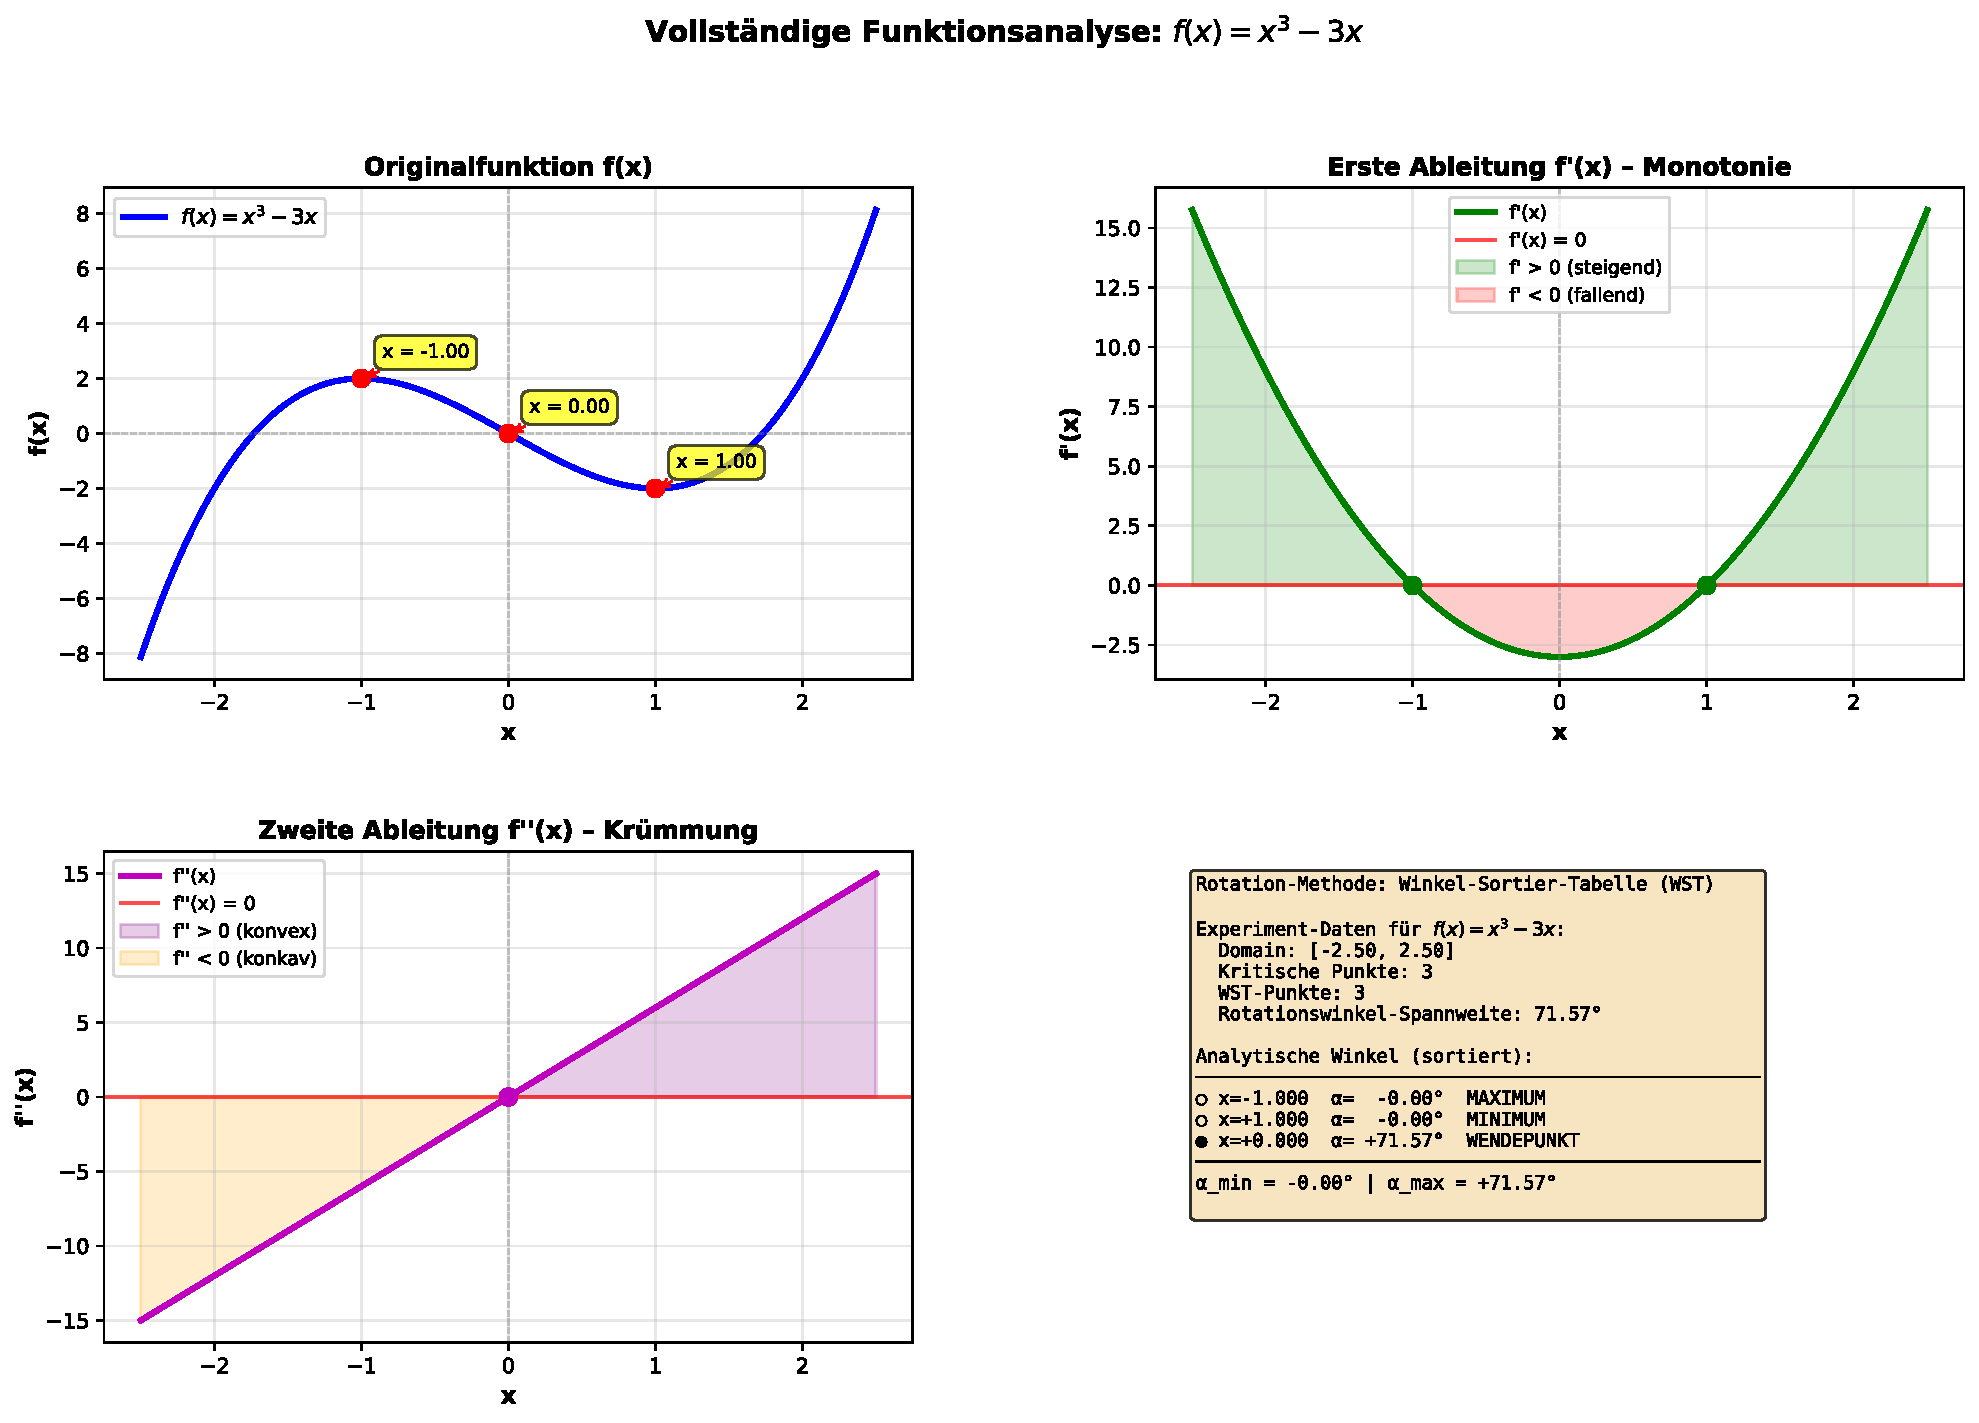
\includegraphics[width=\textwidth]{01_analysis_f1_cubic.pdf}
		\caption{
			\textbf{Vollständige Funktionsanalyse von $f_1(x) = x^3 - 3x$.}
			\emph{Oben-Links:} Originalfunktion mit kritischen Punkten markiert.
			\emph{Oben-Rechts:} Erste Ableitung $f_1'(x)$ mit Monotonie-Regionen (grün = steigend, rot = fallend).
			\emph{Unten-Links:} Zweite Ableitung $f_1''(x)$ mit Krümmungsregionen (violett = konvex, orange = konkav).
			\emph{Unten-Rechts:} Winkel-Sortier-Tabelle (WST) mit analytischen Winkeln und Klassifikationen.
		}
		\label{fig:exp1_analysis}
	\end{figure}
	
	Die Abbildung~\ref{fig:exp1_analysis} zeigt alle vier analytischen Aspekte von $f_1$ zusammen:
	Der Graph hat zwei Extrema bei $x = \pm 1$ mit horizontaler Tangente ($m=0$)
	und einen Wendepunkt bei $x=0$ mit steilster Steigung ($m=-3$).
	
	\begin{figure}[h]
		\centering
		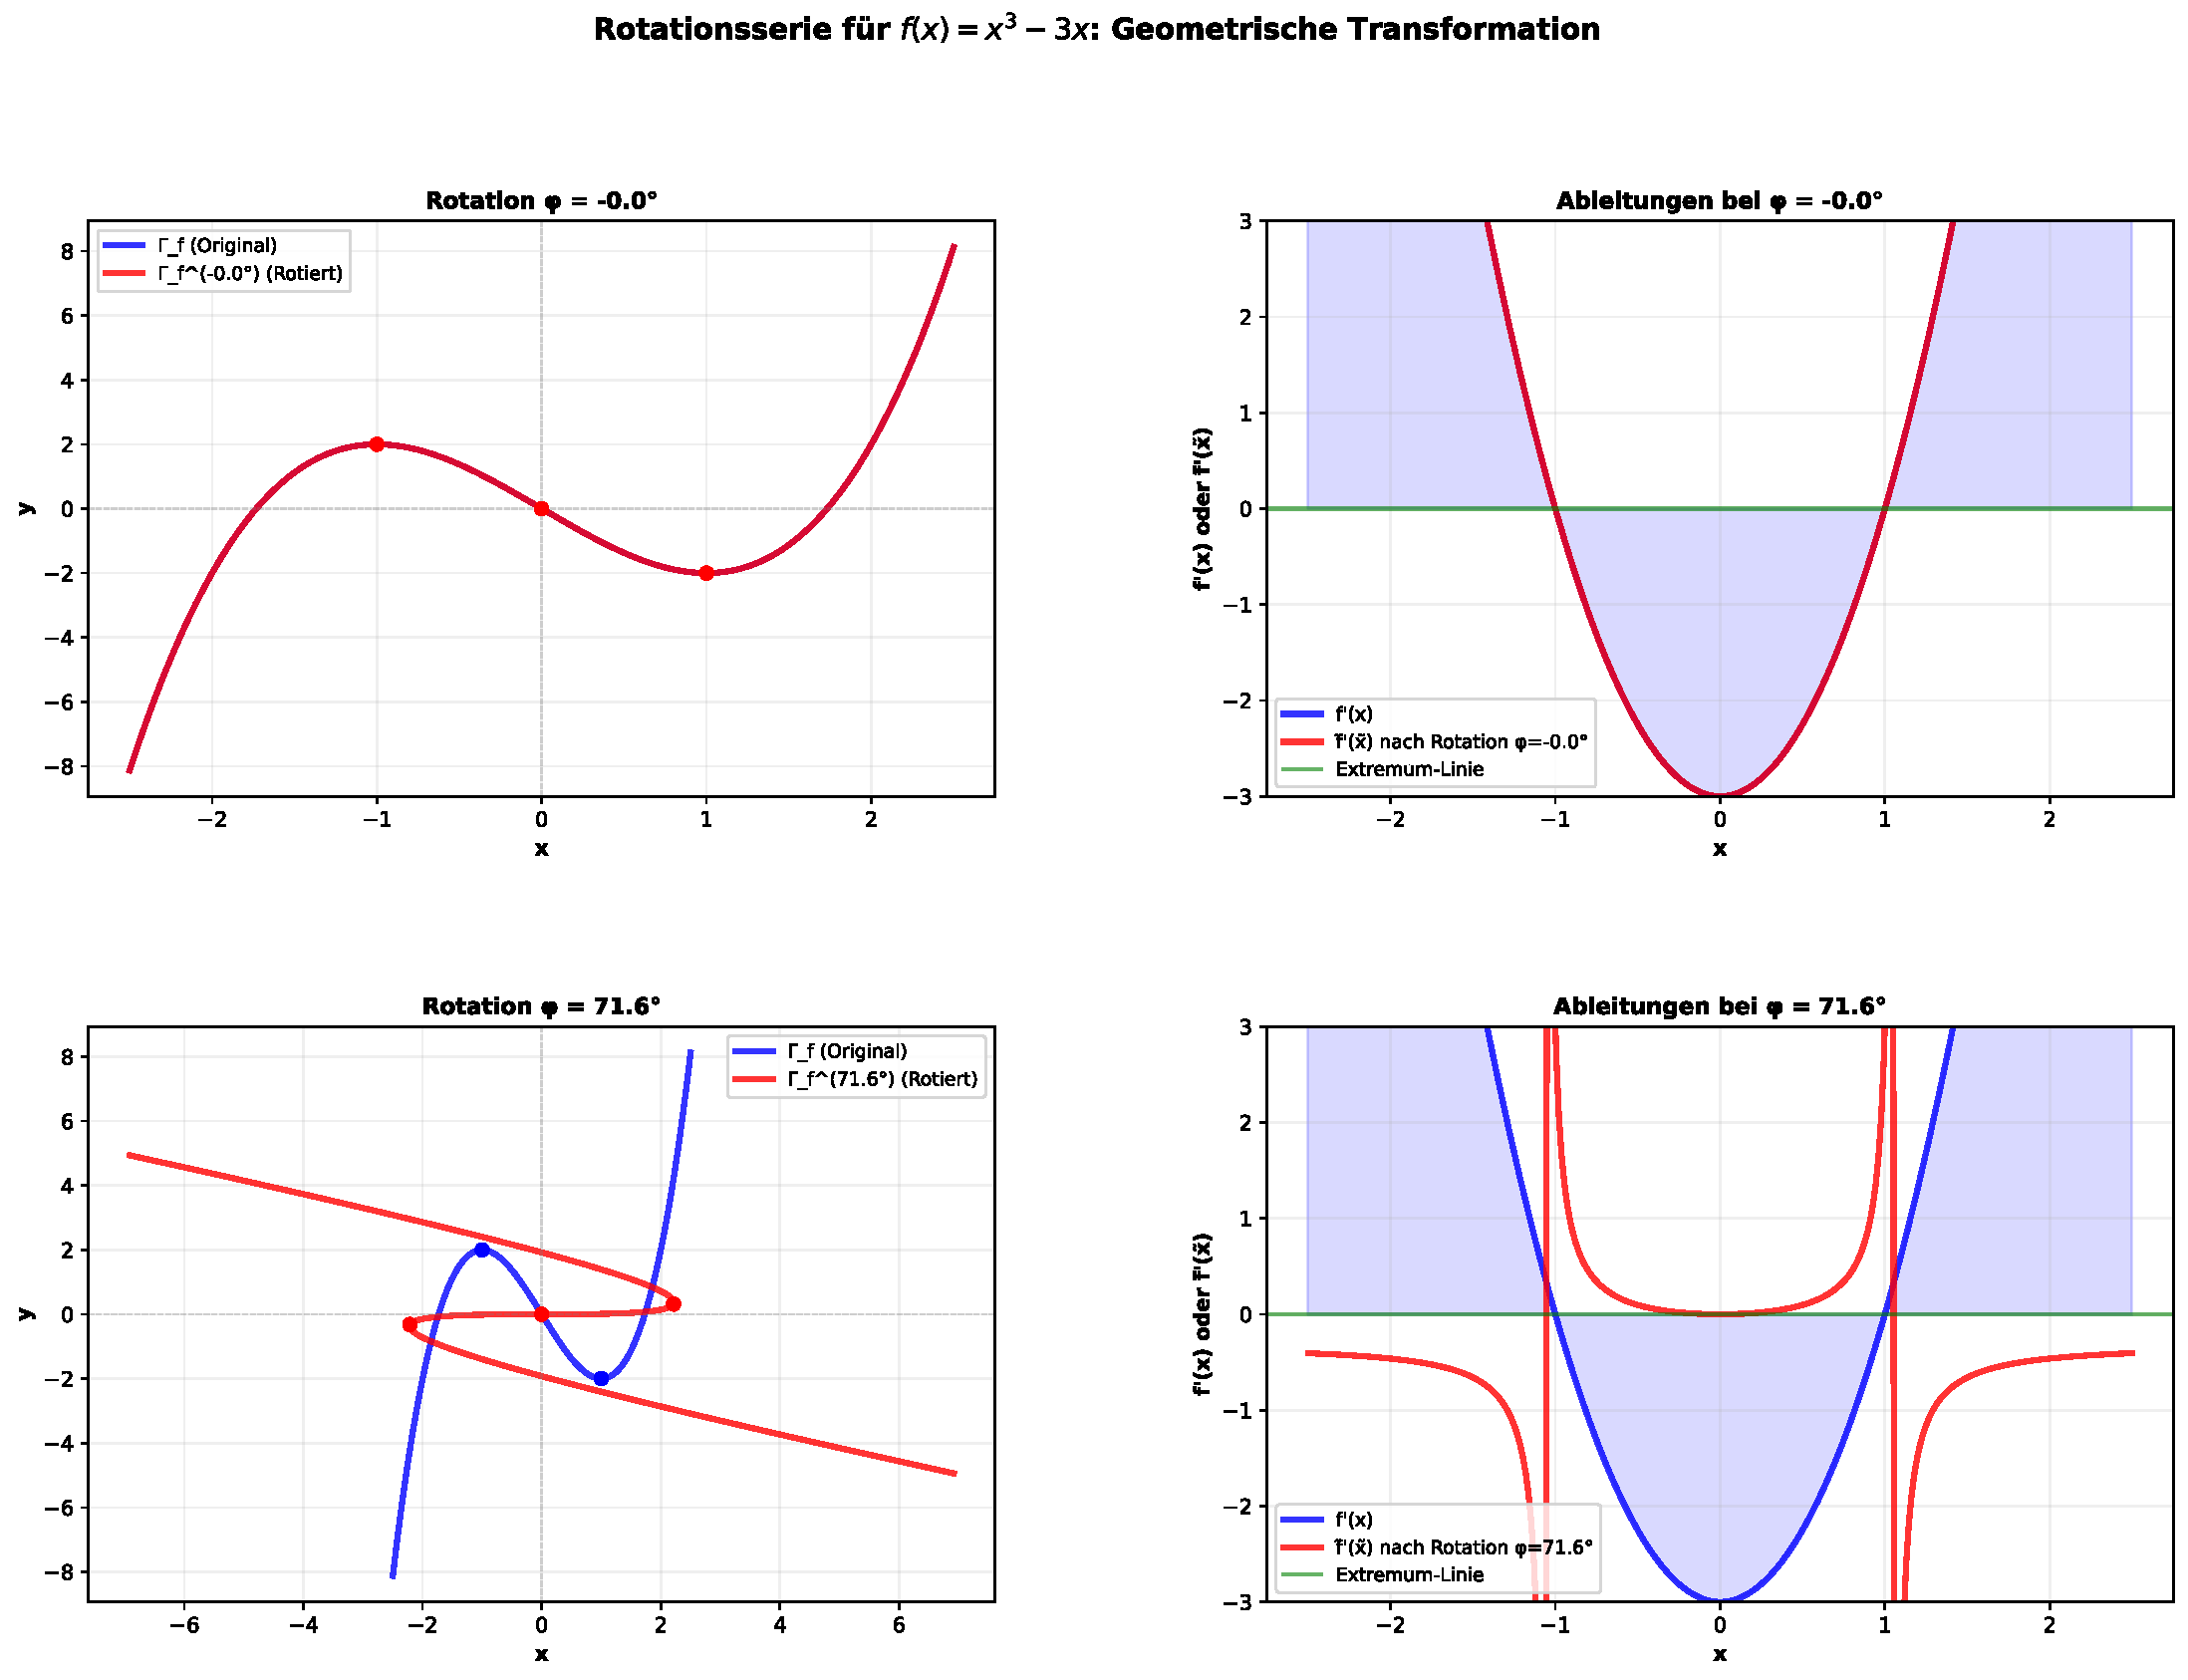
\includegraphics[width=\textwidth]{02_rotation_series_f1_cubic.pdf}
		\caption{
			\textbf{Rotationsserie für $f_1(x) = x^3 - 3x$ bei verschiedenen Winkeln.}
			Für jeden Rotationswinkel (oben-links) werden der Original- (blau) und der rotierte Graph (rot) nebeneinander gezeigt.
			Auf der rechten Seite werden die entsprechenden Ableitungen $f_1'(x)$ (blau) und die rotierte Ableitung $\tilde{f}_1'(\tilde{x})$ (rot) verglichen.
			Die grüne Linie zeigt den Extremum-Bereich ($f' = 0$). Beachte: Wendepunkte von $f_1$ werden zu lokalen Extrema von $\tilde{f}_1$.
		}
		\label{fig:exp1_rotation}
	\end{figure}
	
	\begin{figure}[h]
		\centering
		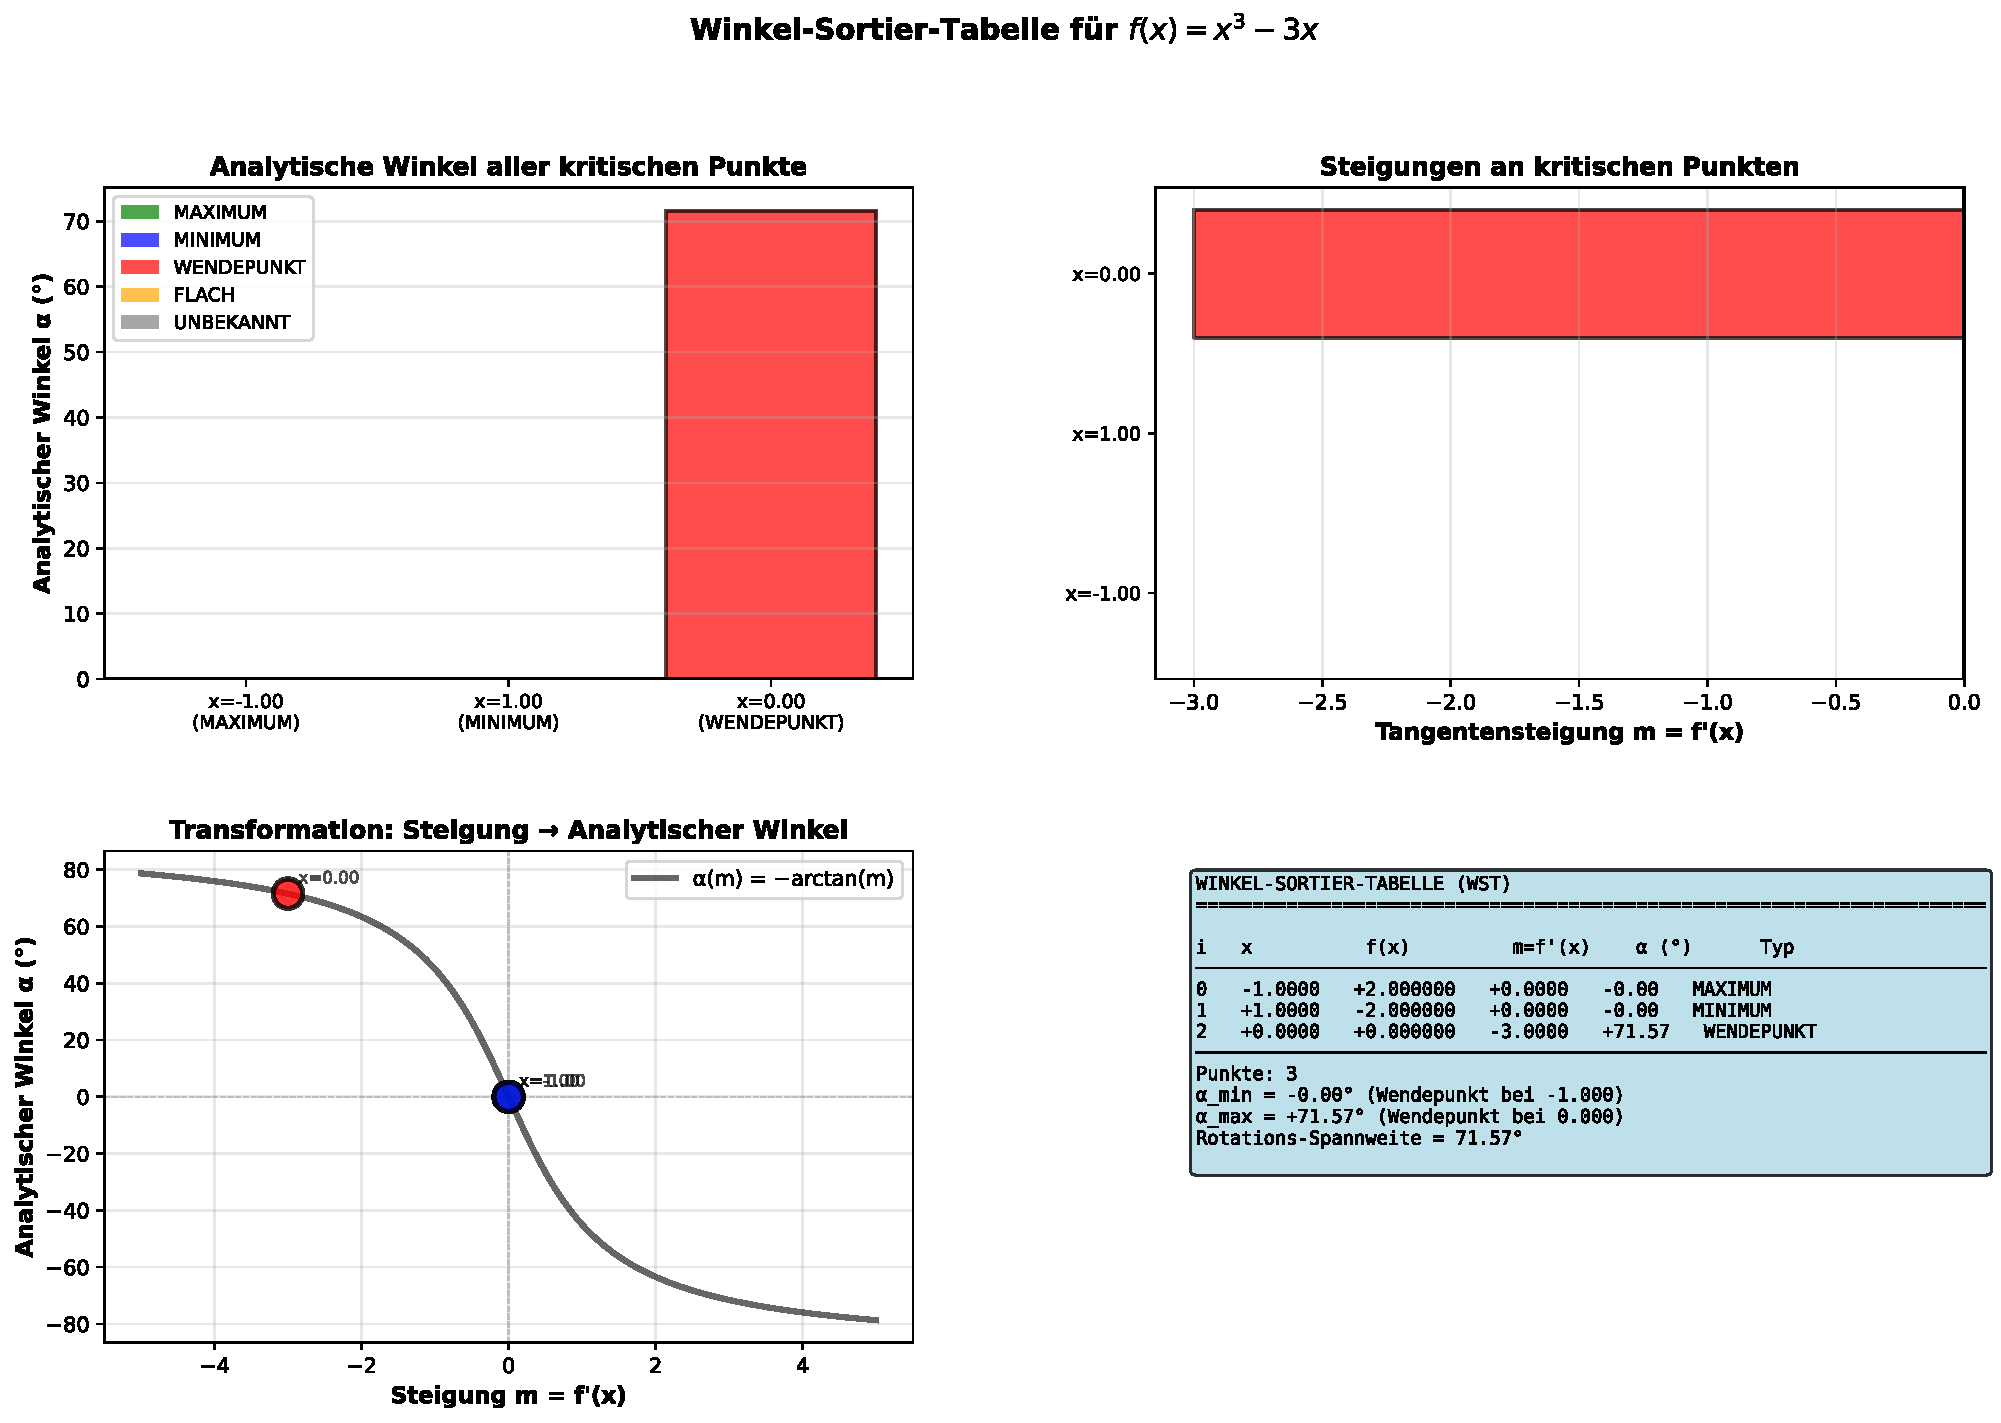
\includegraphics[width=\textwidth]{04_wst_visualization_f1_cubic.pdf}
		\caption{
			\textbf{Winkel-Sortier-Tabelle (WST) für $f_1(x) = x^3 - 3x$ mit visuellen Analysen.}
			\emph{Oben-Links:} Säulendiagramm der analytischen Winkel $\alpha_i$ (sortiert nach Größe).
			\emph{Oben-Rechts:} Steigungen $m_i = f_1'(x_i)$ an den kritischen Punkten.
			\emph{Unten-Links:} Funktionales Verhalten $\alpha(m) = -\arctan(m)$ (schwarze Kurve) mit empirischen Datenpunkten (farbig).
			\emph{Unten-Rechts:} Tabellarische WST mit exakten Zahlenwerten und Klassifikationen.
		}
		\label{fig:exp1_wst}
	\end{figure}
	
	\subsection{Experiment 2: Quintische Funktion $f_2(x) = x^5 - 5x^3 + 4x$}
	\label{subsec:exp2}
	
	Die zweite Testfunktion ist eine Polynom fünften Grades mit zwei Wendepunkten,
	die die Komplexität der WST-Methode für mehrkritische Funktionen demonstriert.
	
	\subsubsection{Analytische Ãœbersicht}
	
	Sei $f_2(x) = x^5 - 5x^3 + 4x$. Dann:
	\begin{align}
		f_2'(x) &= 5x^4 - 15x^2 + 4, \\
		f_2''(x) &= 20x^3 - 30x = 10x(2x^2 - 3).
	\end{align}
	
	Die zweite Ableitung verschwindet bei $x \in \{-\sqrt{3/2}, 0, +\sqrt{3/2}\} \approx \{-1.225, 0, +1.225\}$.
	
	Kritische Punkte und ihre Klassifikation:
	\begin{itemize}
		\item $x = -1$: Wendepunkt, $f_2(-1) = 0$, $f_2'(-1) = 5 - 15 + 4 = -6$, $\alpha \approx +80.54°$
		\item $x = 0$: Wendepunkt, $f_2(0) = 0$, $f_2'(0) = 4$, $\alpha \approx -75.96°$
		\item $x = +1$: Wendepunkt, $f_2(1) = 0$, $f_2'(1) = -6$, $\alpha \approx +80.54°$
	\end{itemize}
	
	Die Rotationsspannweite beträgt $\Delta \alpha \approx 156.50°$, womit fast eine halbe
	Drehung erforderlich ist, um alle Wendepunkte als Extrema der rotierten Kurve zu erfassen.
	
	\subsubsection{Visualisierungen}
	
	\begin{figure}[h]
		\centering
		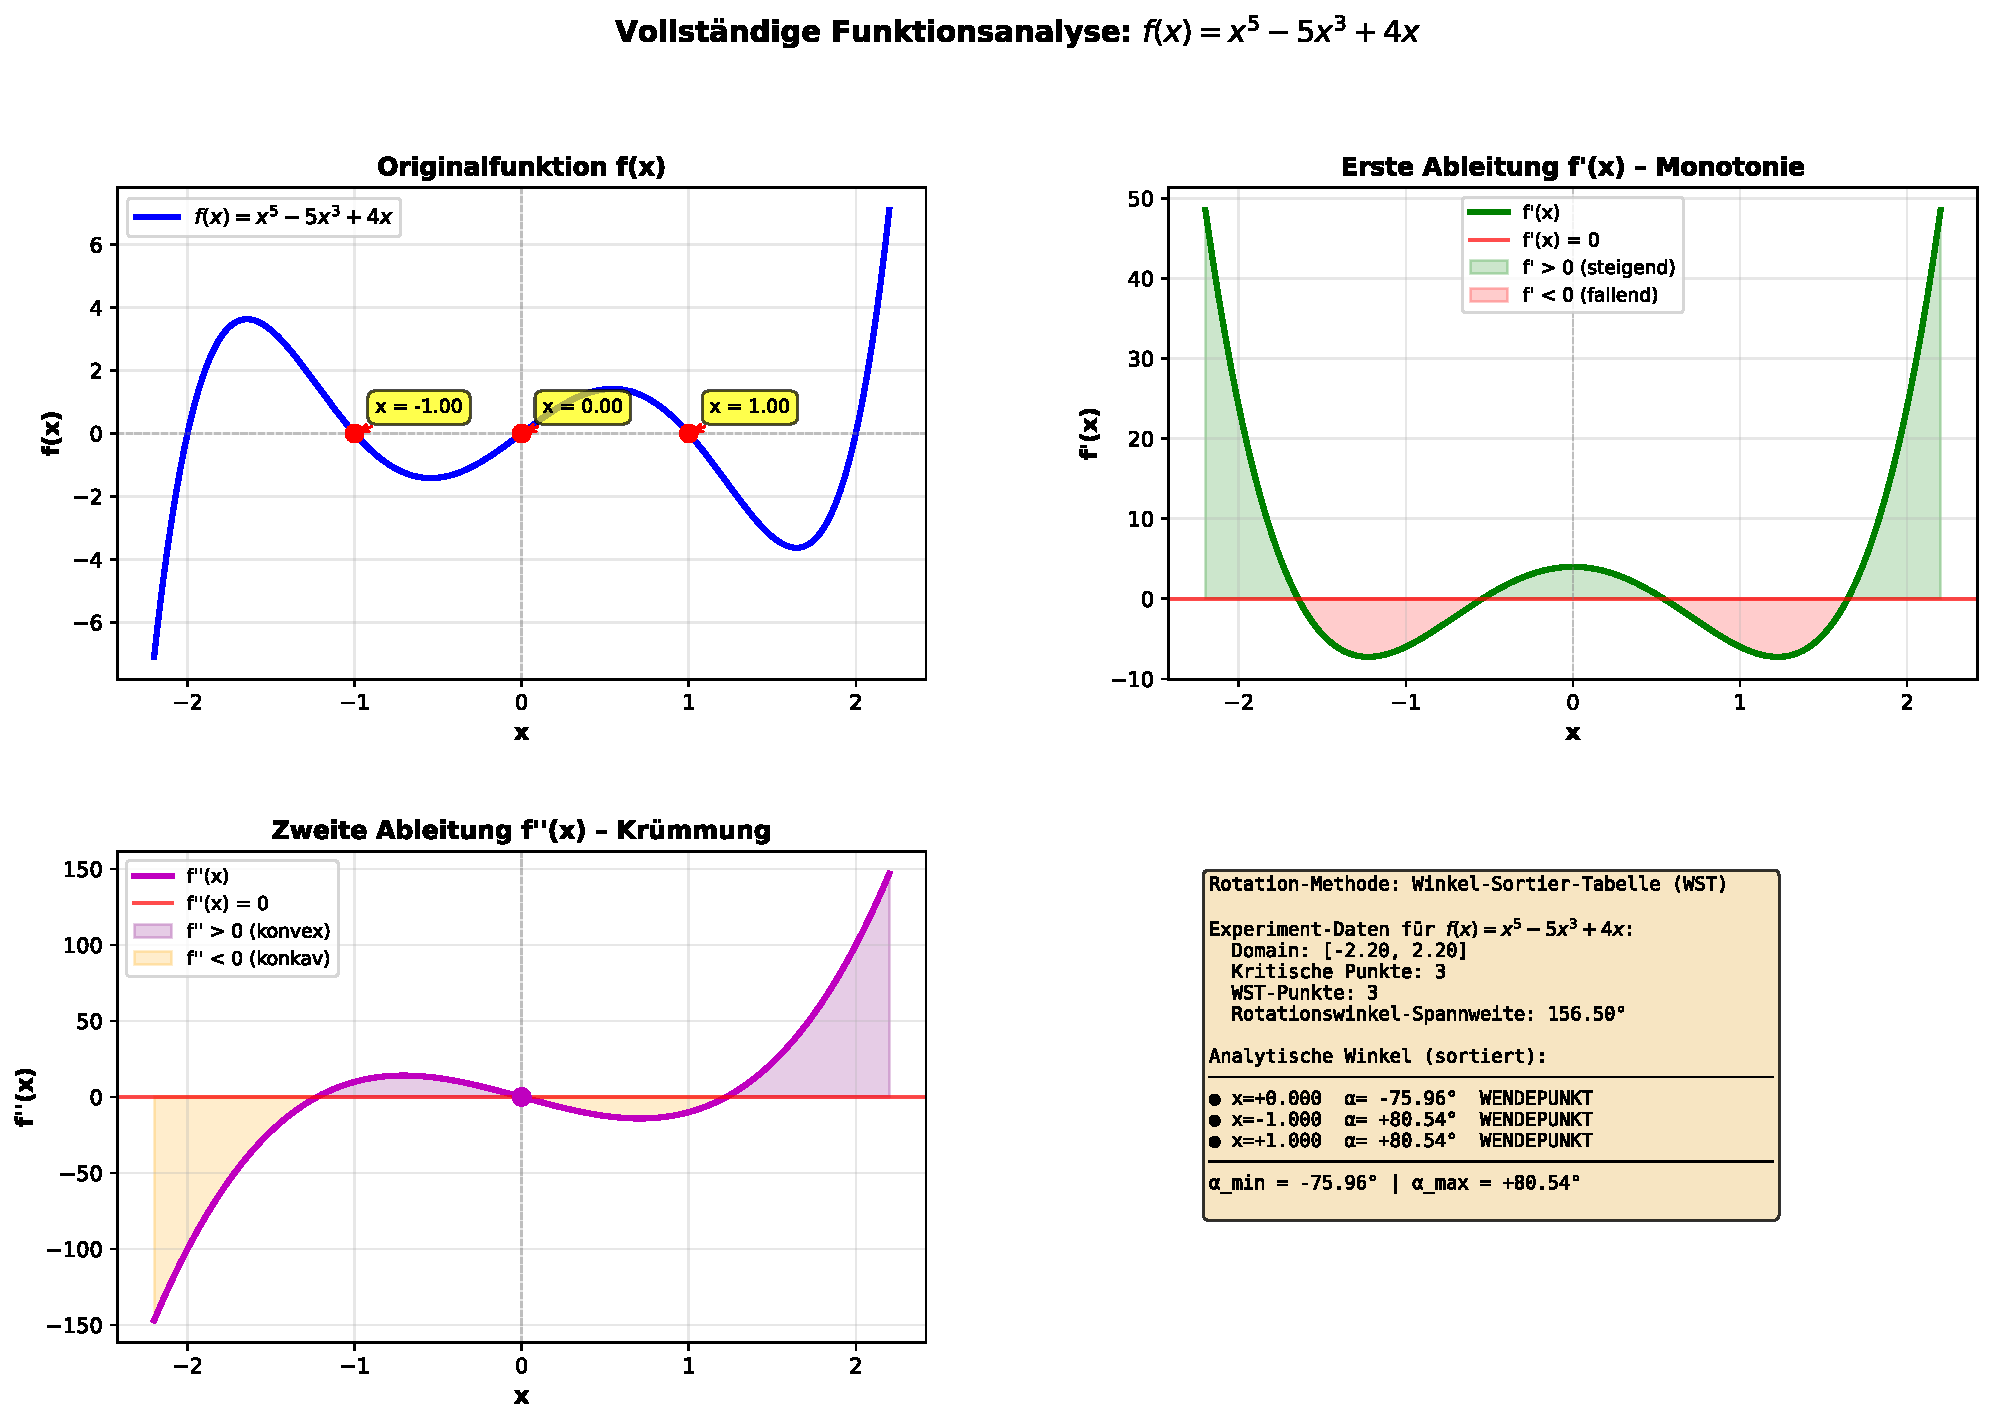
\includegraphics[width=\textwidth]{01_analysis_f2_quintic.pdf}
		\caption{
			\textbf{Vollständige Funktionsanalyse von $f_2(x) = x^5 - 5x^3 + 4x$.}
			Diese quintische Funktion hat drei kritische Punkte mit unterschiedlichen analytischen Winkeln.
			Die erste Ableitung zeigt zwei Extrema (lokales Maximum bei $x \approx -0.7$ und Minimum bei $x \approx +0.7$).
			Die zweite Ableitung hat drei Nullstellen, die Wendepunkte anzeigen.
		}
		\label{fig:exp2_analysis}
	\end{figure}
	
	\begin{figure}[h]
		\centering
		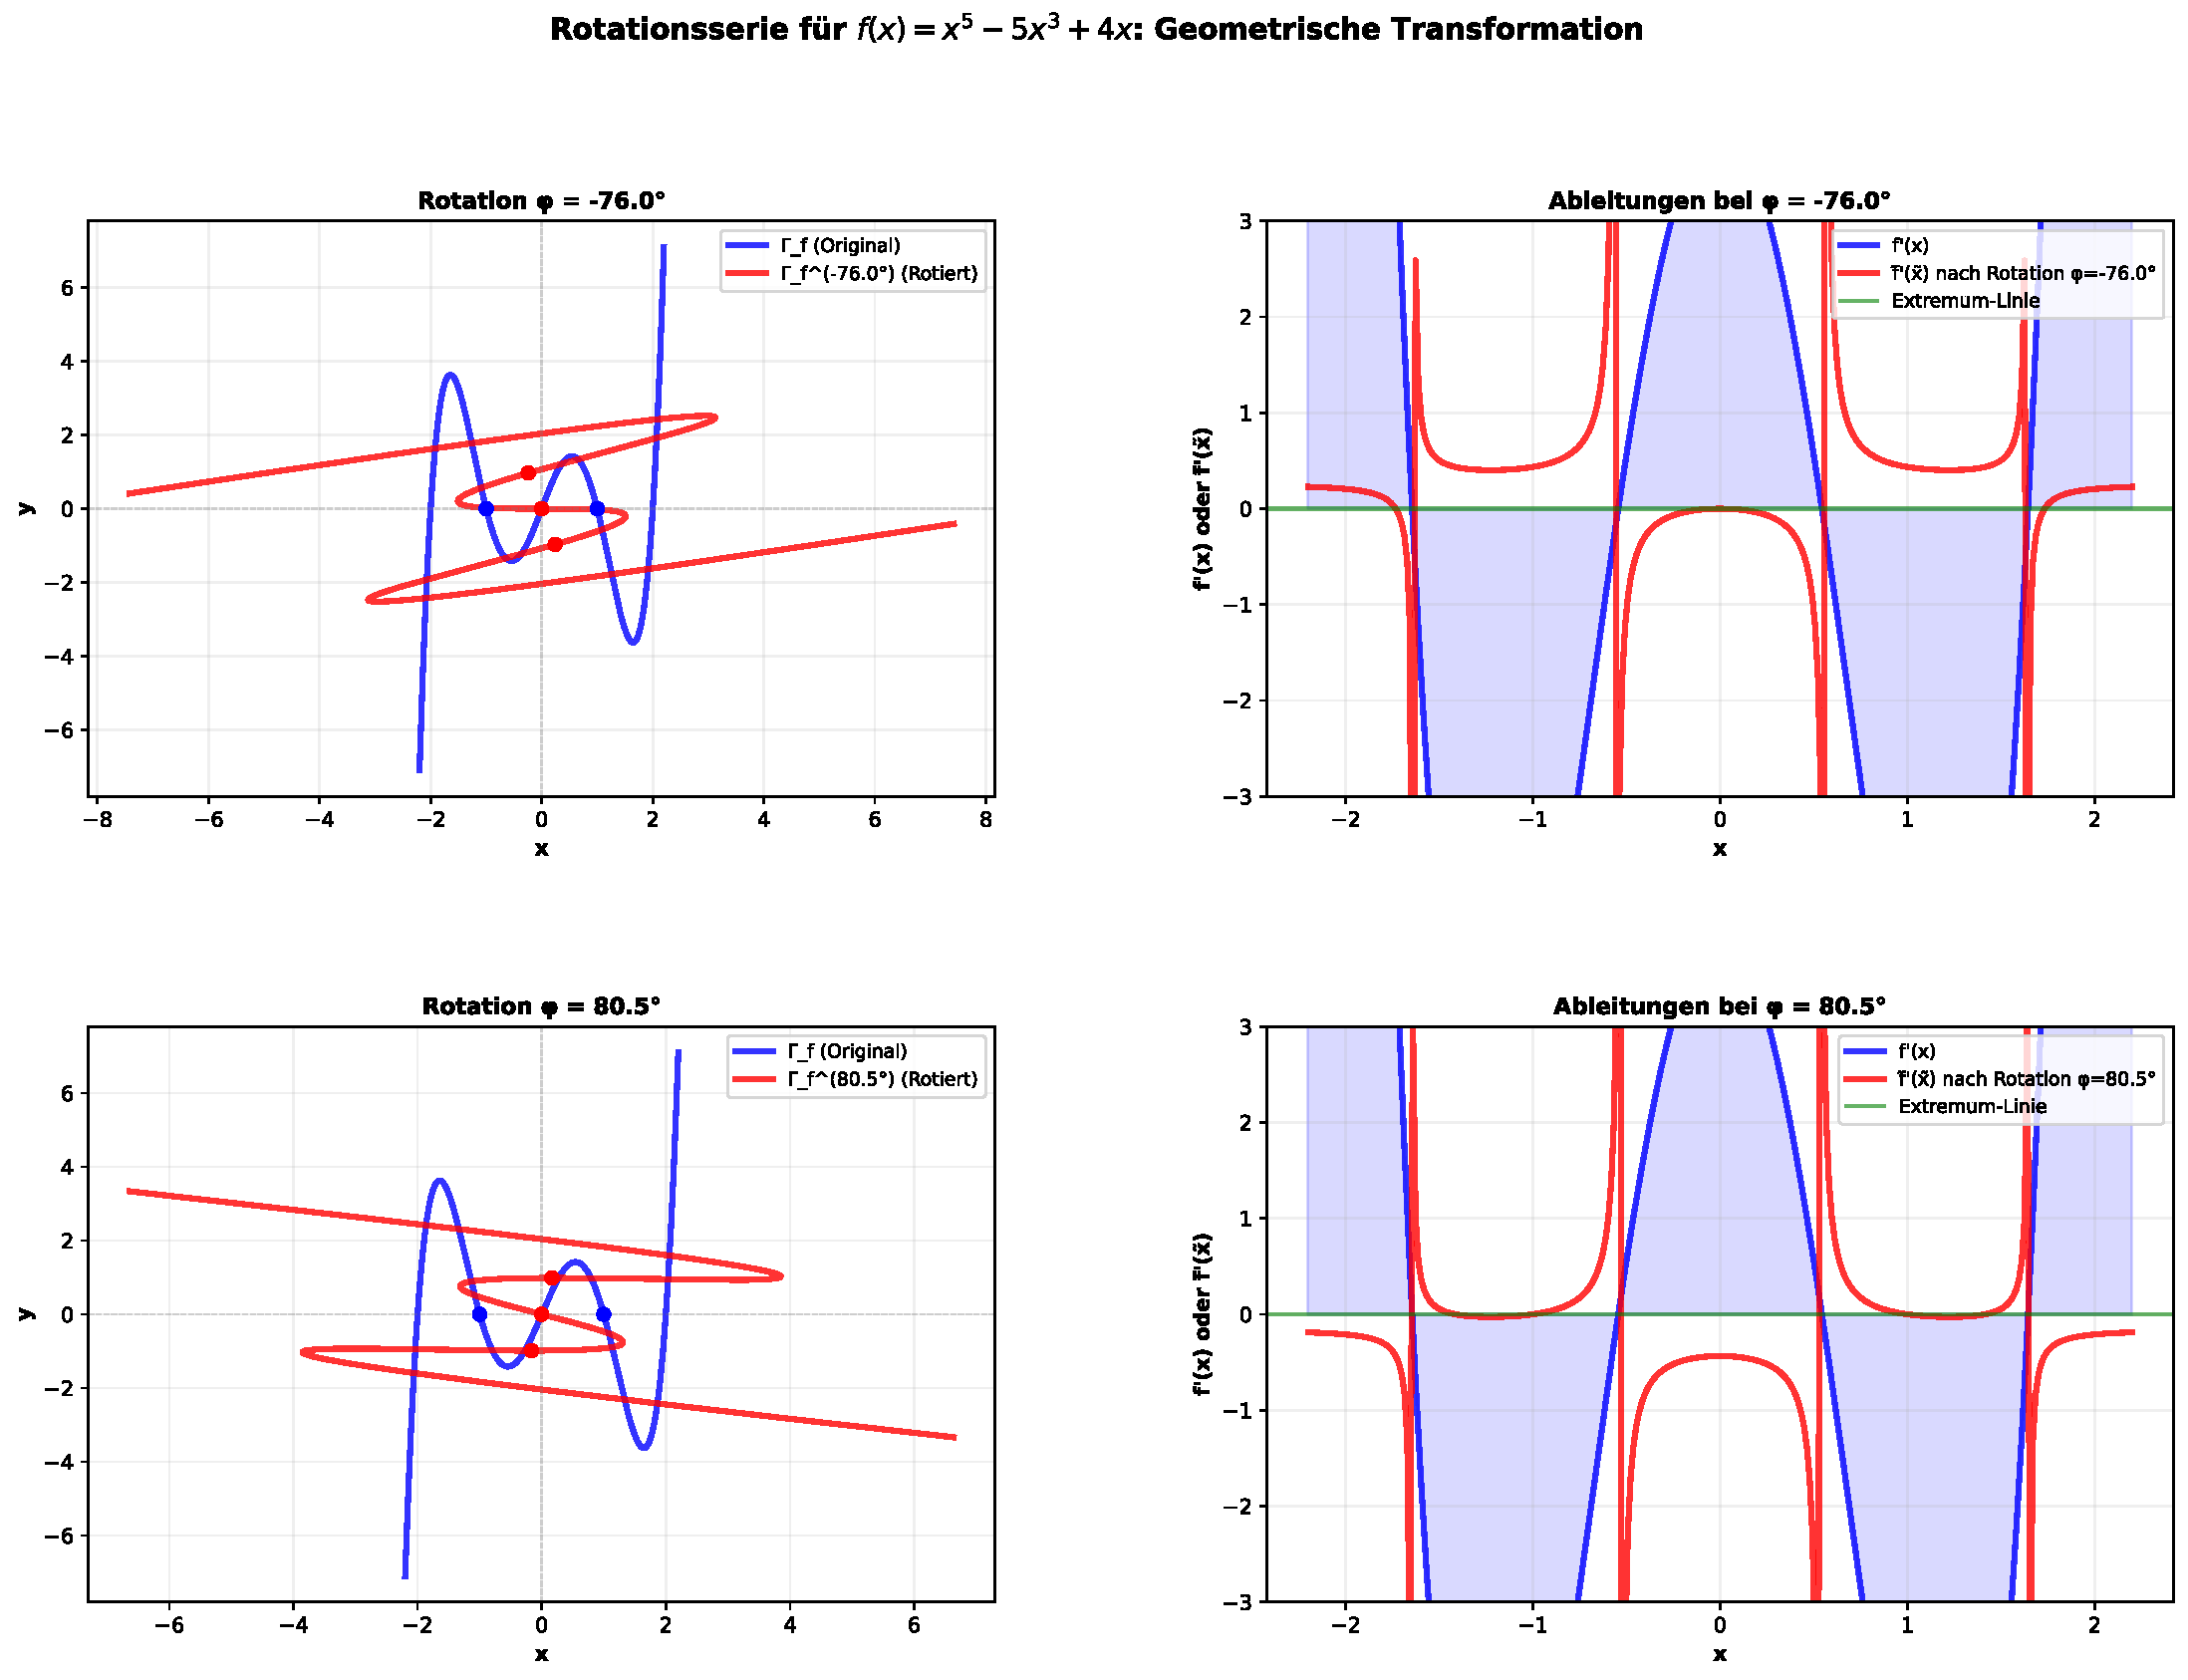
\includegraphics[width=\textwidth]{02_rotation_series_f2_quintic.pdf}
		\caption{
			\textbf{Rotationsserie für $f_2(x) = x^5 - 5x^3 + 4x$.}
			Die Serie zeigt, wie sich die rotierten Ableitungen $\tilde{f}_2'$ bei verschiedenen Winkeln ändern.
			Bei den analytischen Winkeln $\alpha \approx \pm 80°$ und $\alpha \approx -76°$ verschwinden die Ableitungen $\tilde{f}_2'(\tilde{x}) = 0$,
			was die Wendepunkte von $f_2$ als Extrema der rotierten Kurve enthüllt.
		}
		\label{fig:exp2_rotation}
	\end{figure}
	
	\begin{figure}[h]
		\centering
		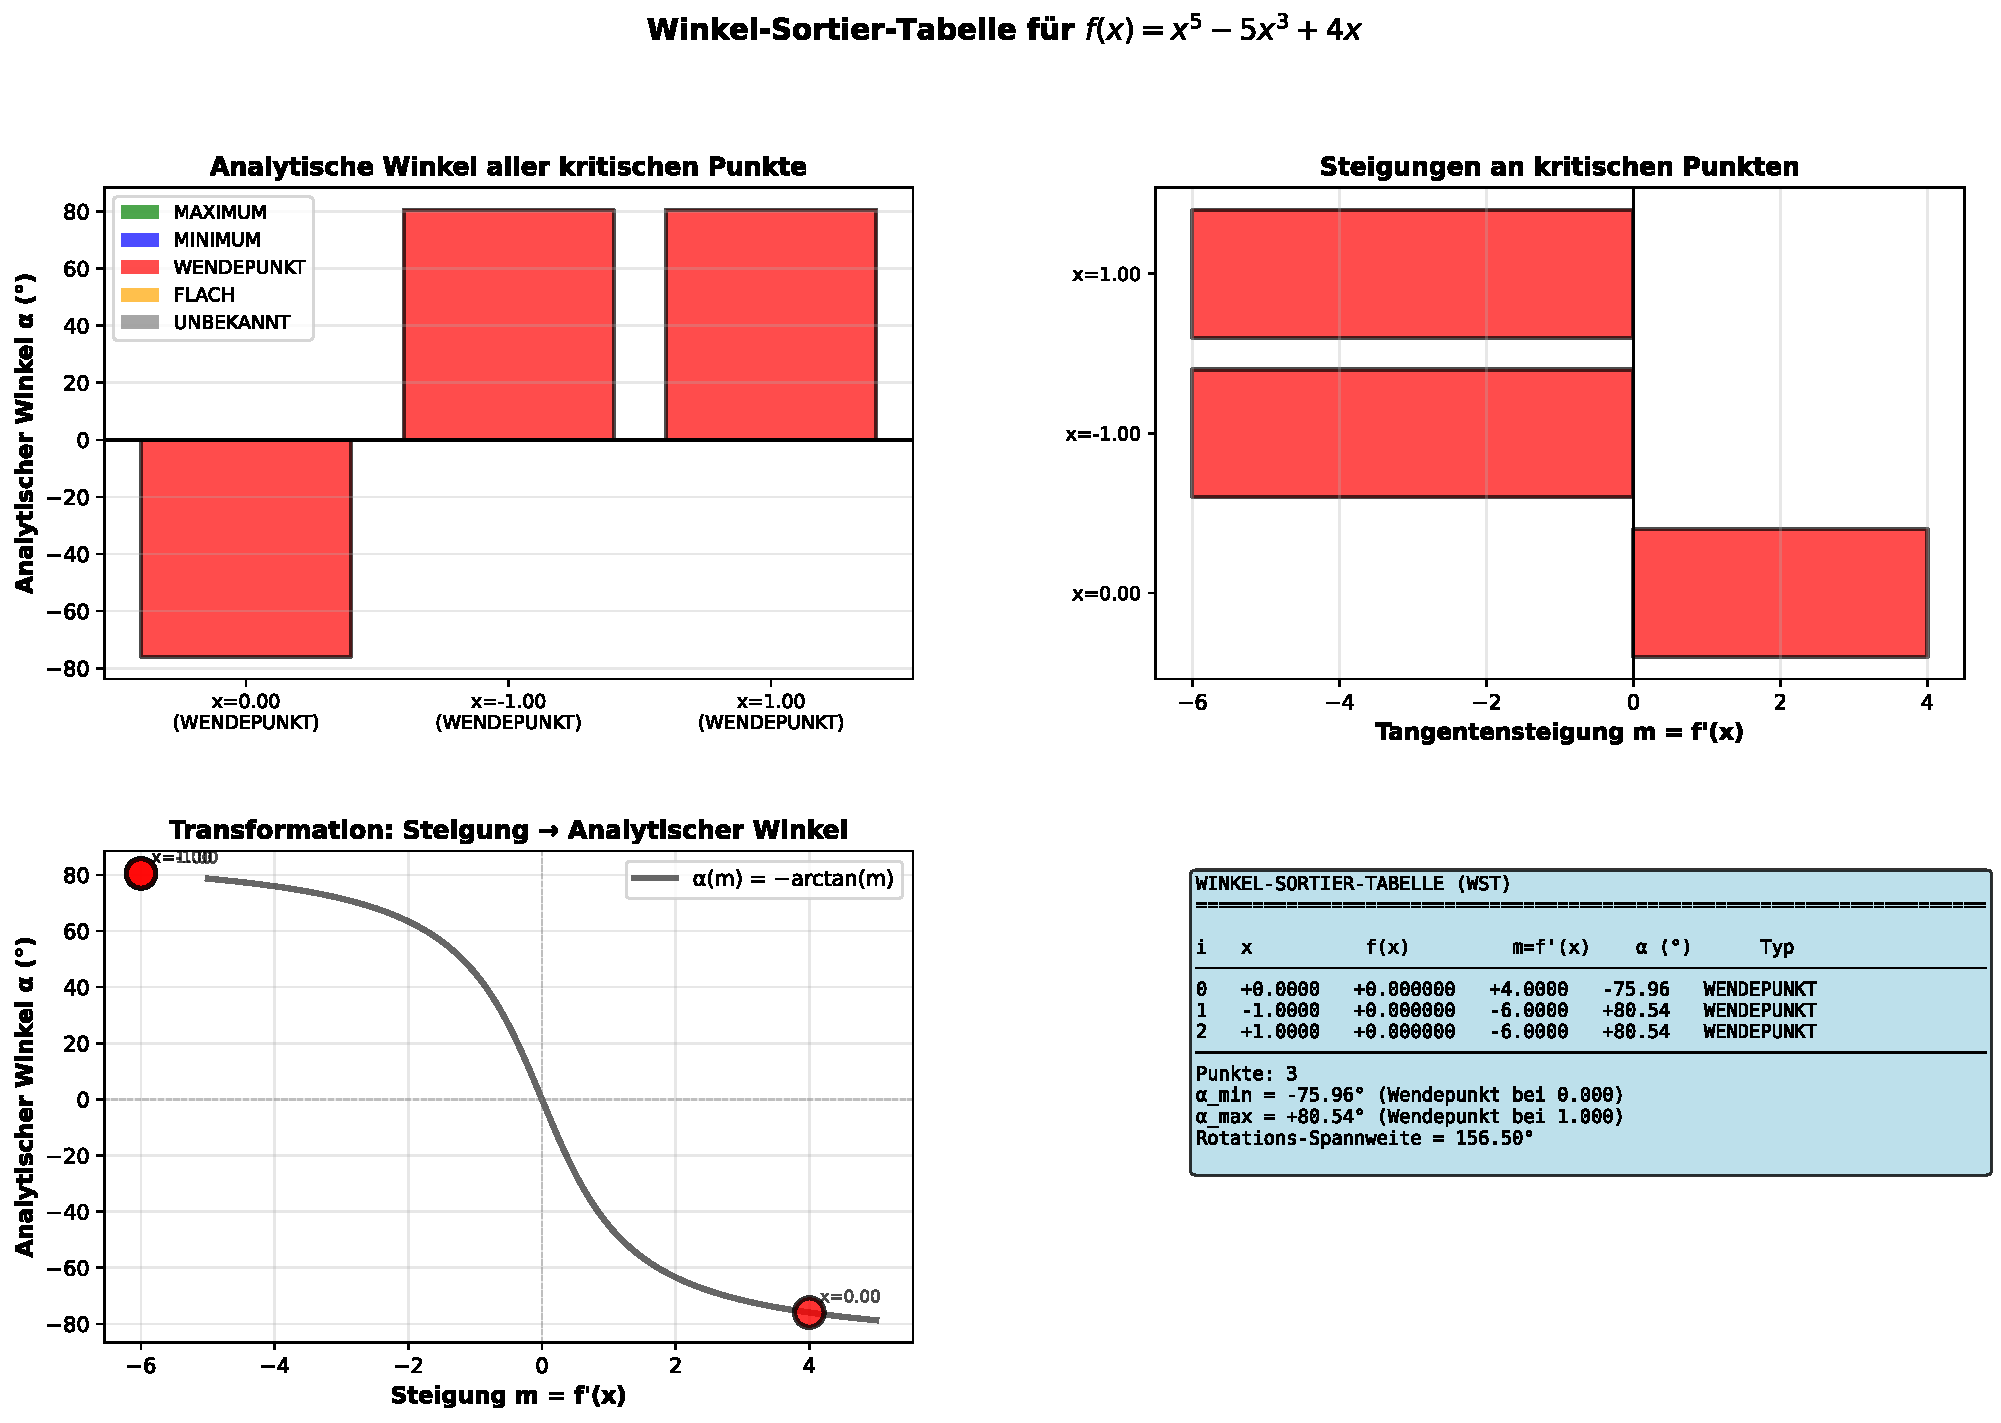
\includegraphics[width=\textwidth]{04_wst_visualization_f2_quintic.pdf}
		\caption{
			\textbf{Winkel-Sortier-Tabelle (WST) für $f_2(x) = x^5 - 5x^3 + 4x$.}
			Die WST zeigt drei Wendepunkte mit Rotationsspannweite $\Delta \alpha \approx 156°$.
			Beachte die symmetrische Struktur: Zwei der Wendepunkte bei $x = \pm 1$ haben identische Steigung $m=-6$ und daher denselben analytischen Winkel.
		}
		\label{fig:exp2_wst}
	\end{figure}
	
	\subsection{Experiment 3: Trigonometrische Funktion $f_3(x) = \sin(x)$}
	\label{subsec:exp3}
	
	Die dritte Testfunktion ist die Sinusfunktion, die zeigt, wie die Rotationsmethode
	auf periodische Funktionen mit unendlich vielen Wendepunkten anwendbar ist.
	
	\subsubsection{Analytische Ãœbersicht}
	
	Sei $f_3(x) = \sin(x)$. Dann:
	\begin{align}
		f_3'(x) &= \cos(x), \\
		f_3''(x) &= -\sin(x).
	\end{align}
	
	Wendepunkte treten überall dort auf, wo $f_3''(x) = 0$, d.\,h.\ bei $x = n\pi$ für $n \in \mathbb{Z}$.
	Die Steigungen bei den Wendepunkten sind:
	\begin{align*}
		f_3'(n\pi) = \cos(n\pi) = (-1)^n \in \{-1, +1\}.
	\end{align*}
	
	Analytische Winkel:
	\begin{align*}
		\text{bei } \cos(x) = 1 \quad (\text{z.B. } x=0): \quad \alpha &= -\arctan(1) = -45° \\
		\text{bei } \cos(x) = -1 \quad (\text{z.B. } x=\pi): \quad \alpha &= -\arctan(-1) = +45°
	\end{align*}
	
	Die Rotationsspannweite zwischen aufeinanderfolgenden Wendepunkttypen beträgt $\Delta \alpha = 90°$.
	
	\subsubsection{Visualisierungen}
	
	\begin{figure}[h]
		\centering
		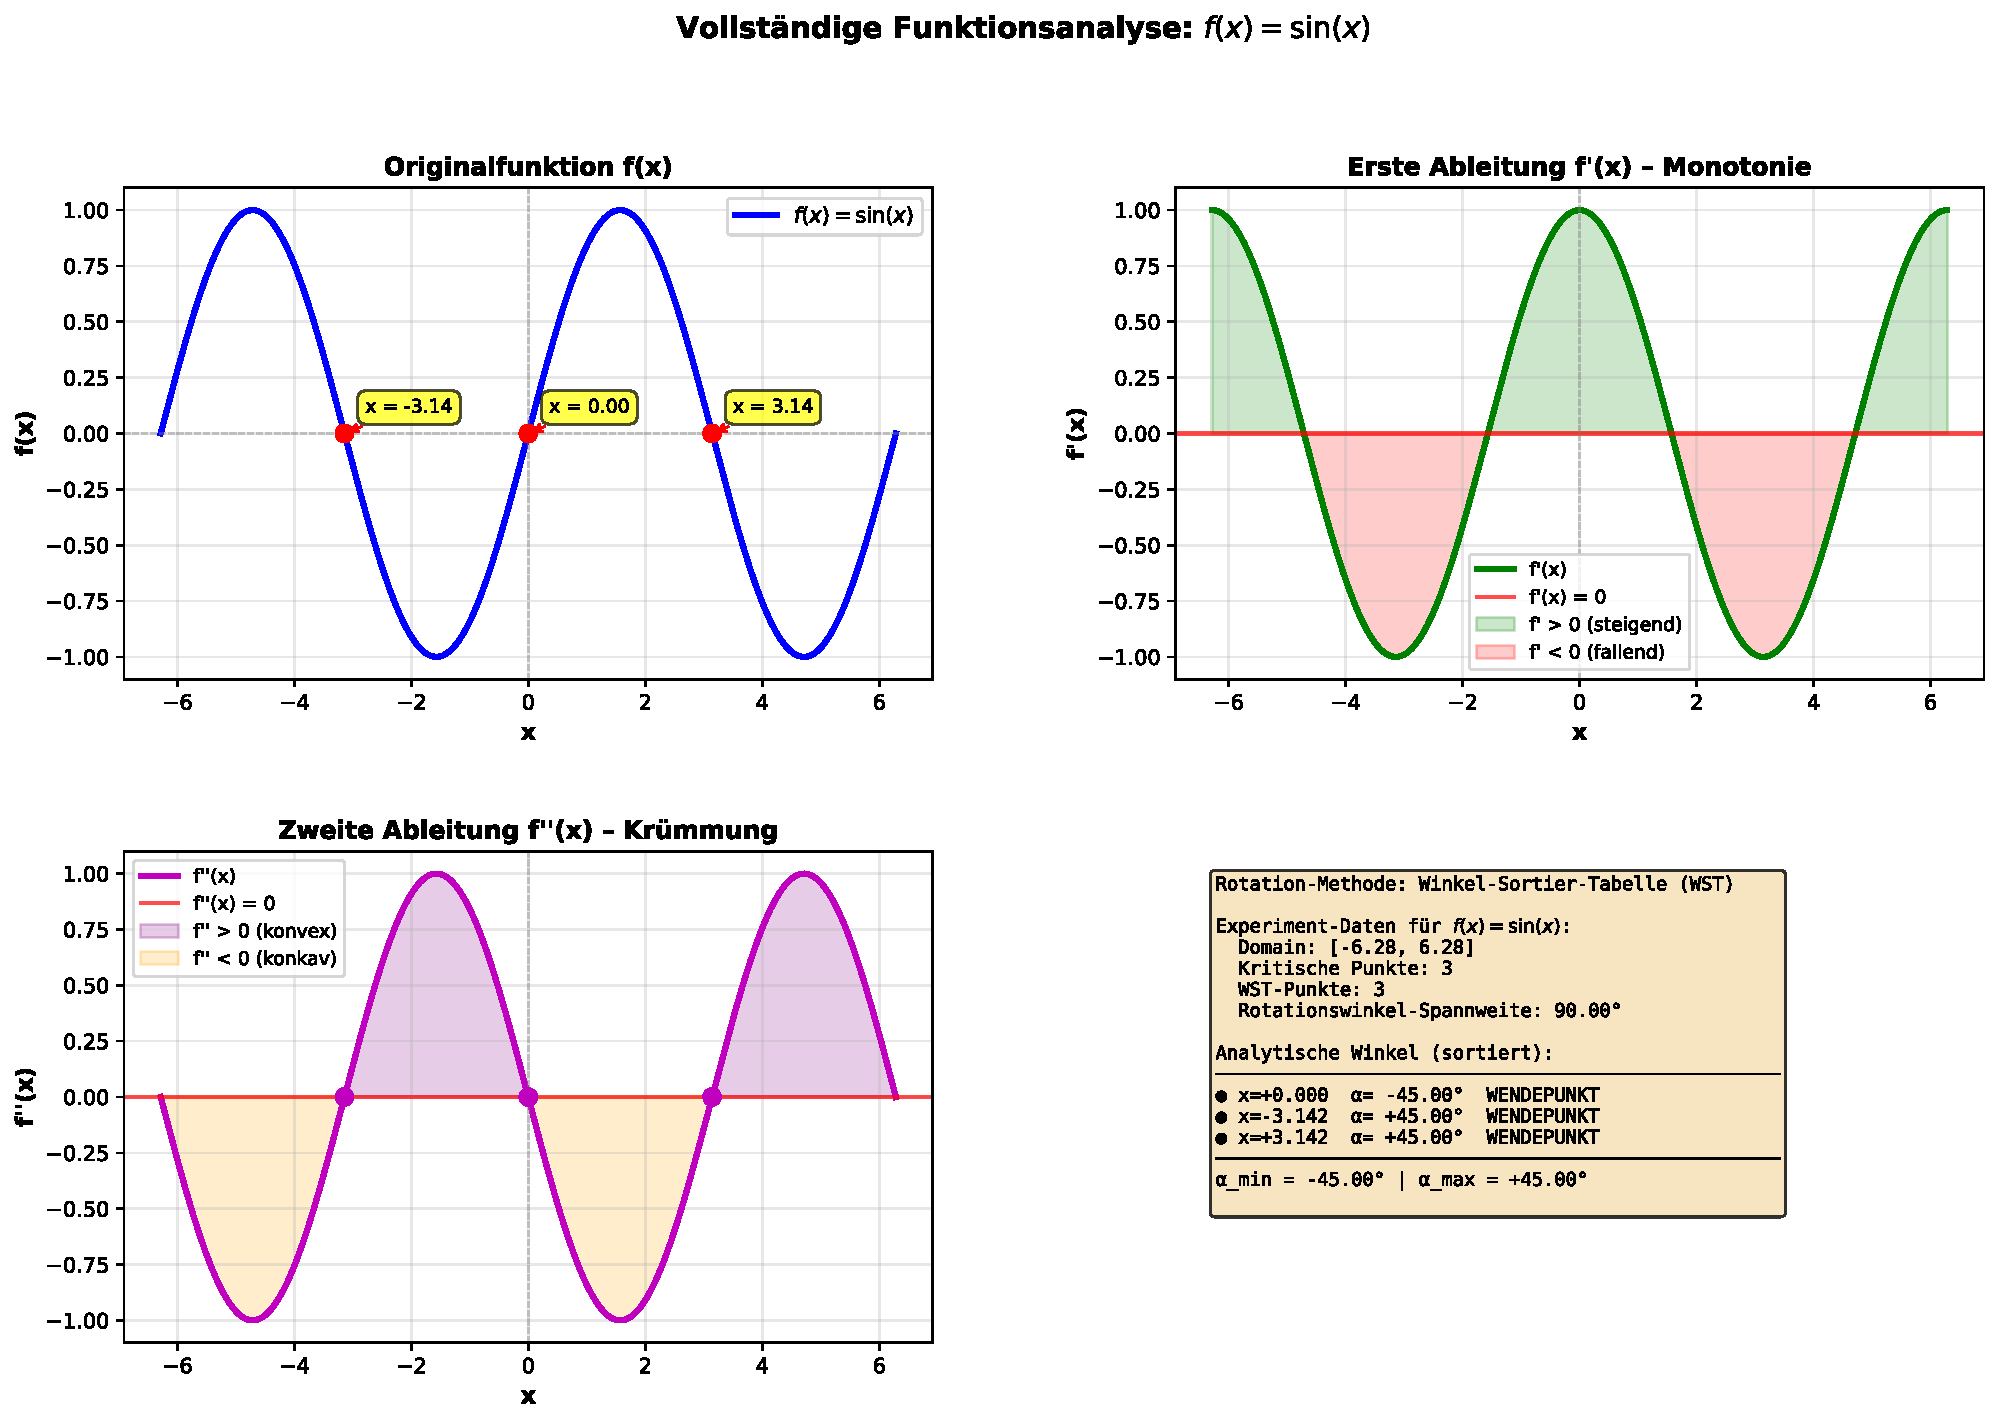
\includegraphics[width=\textwidth]{01_analysis_f3_sine.pdf}
		\caption{
			\textbf{Vollständige Funktionsanalyse von $f_3(x) = \sin(x)$.}
			Die periodische Natur von Sinus zeigt sich in allen vier Diagrammen.
			Extrema bei $x \approx \pm \pi/2$ wechseln sich mit Wendepunkten bei $x \approx 0, \pm \pi$ ab.
		}
		\label{fig:exp3_analysis}
	\end{figure}
	
	\begin{figure}[h]
		\centering
		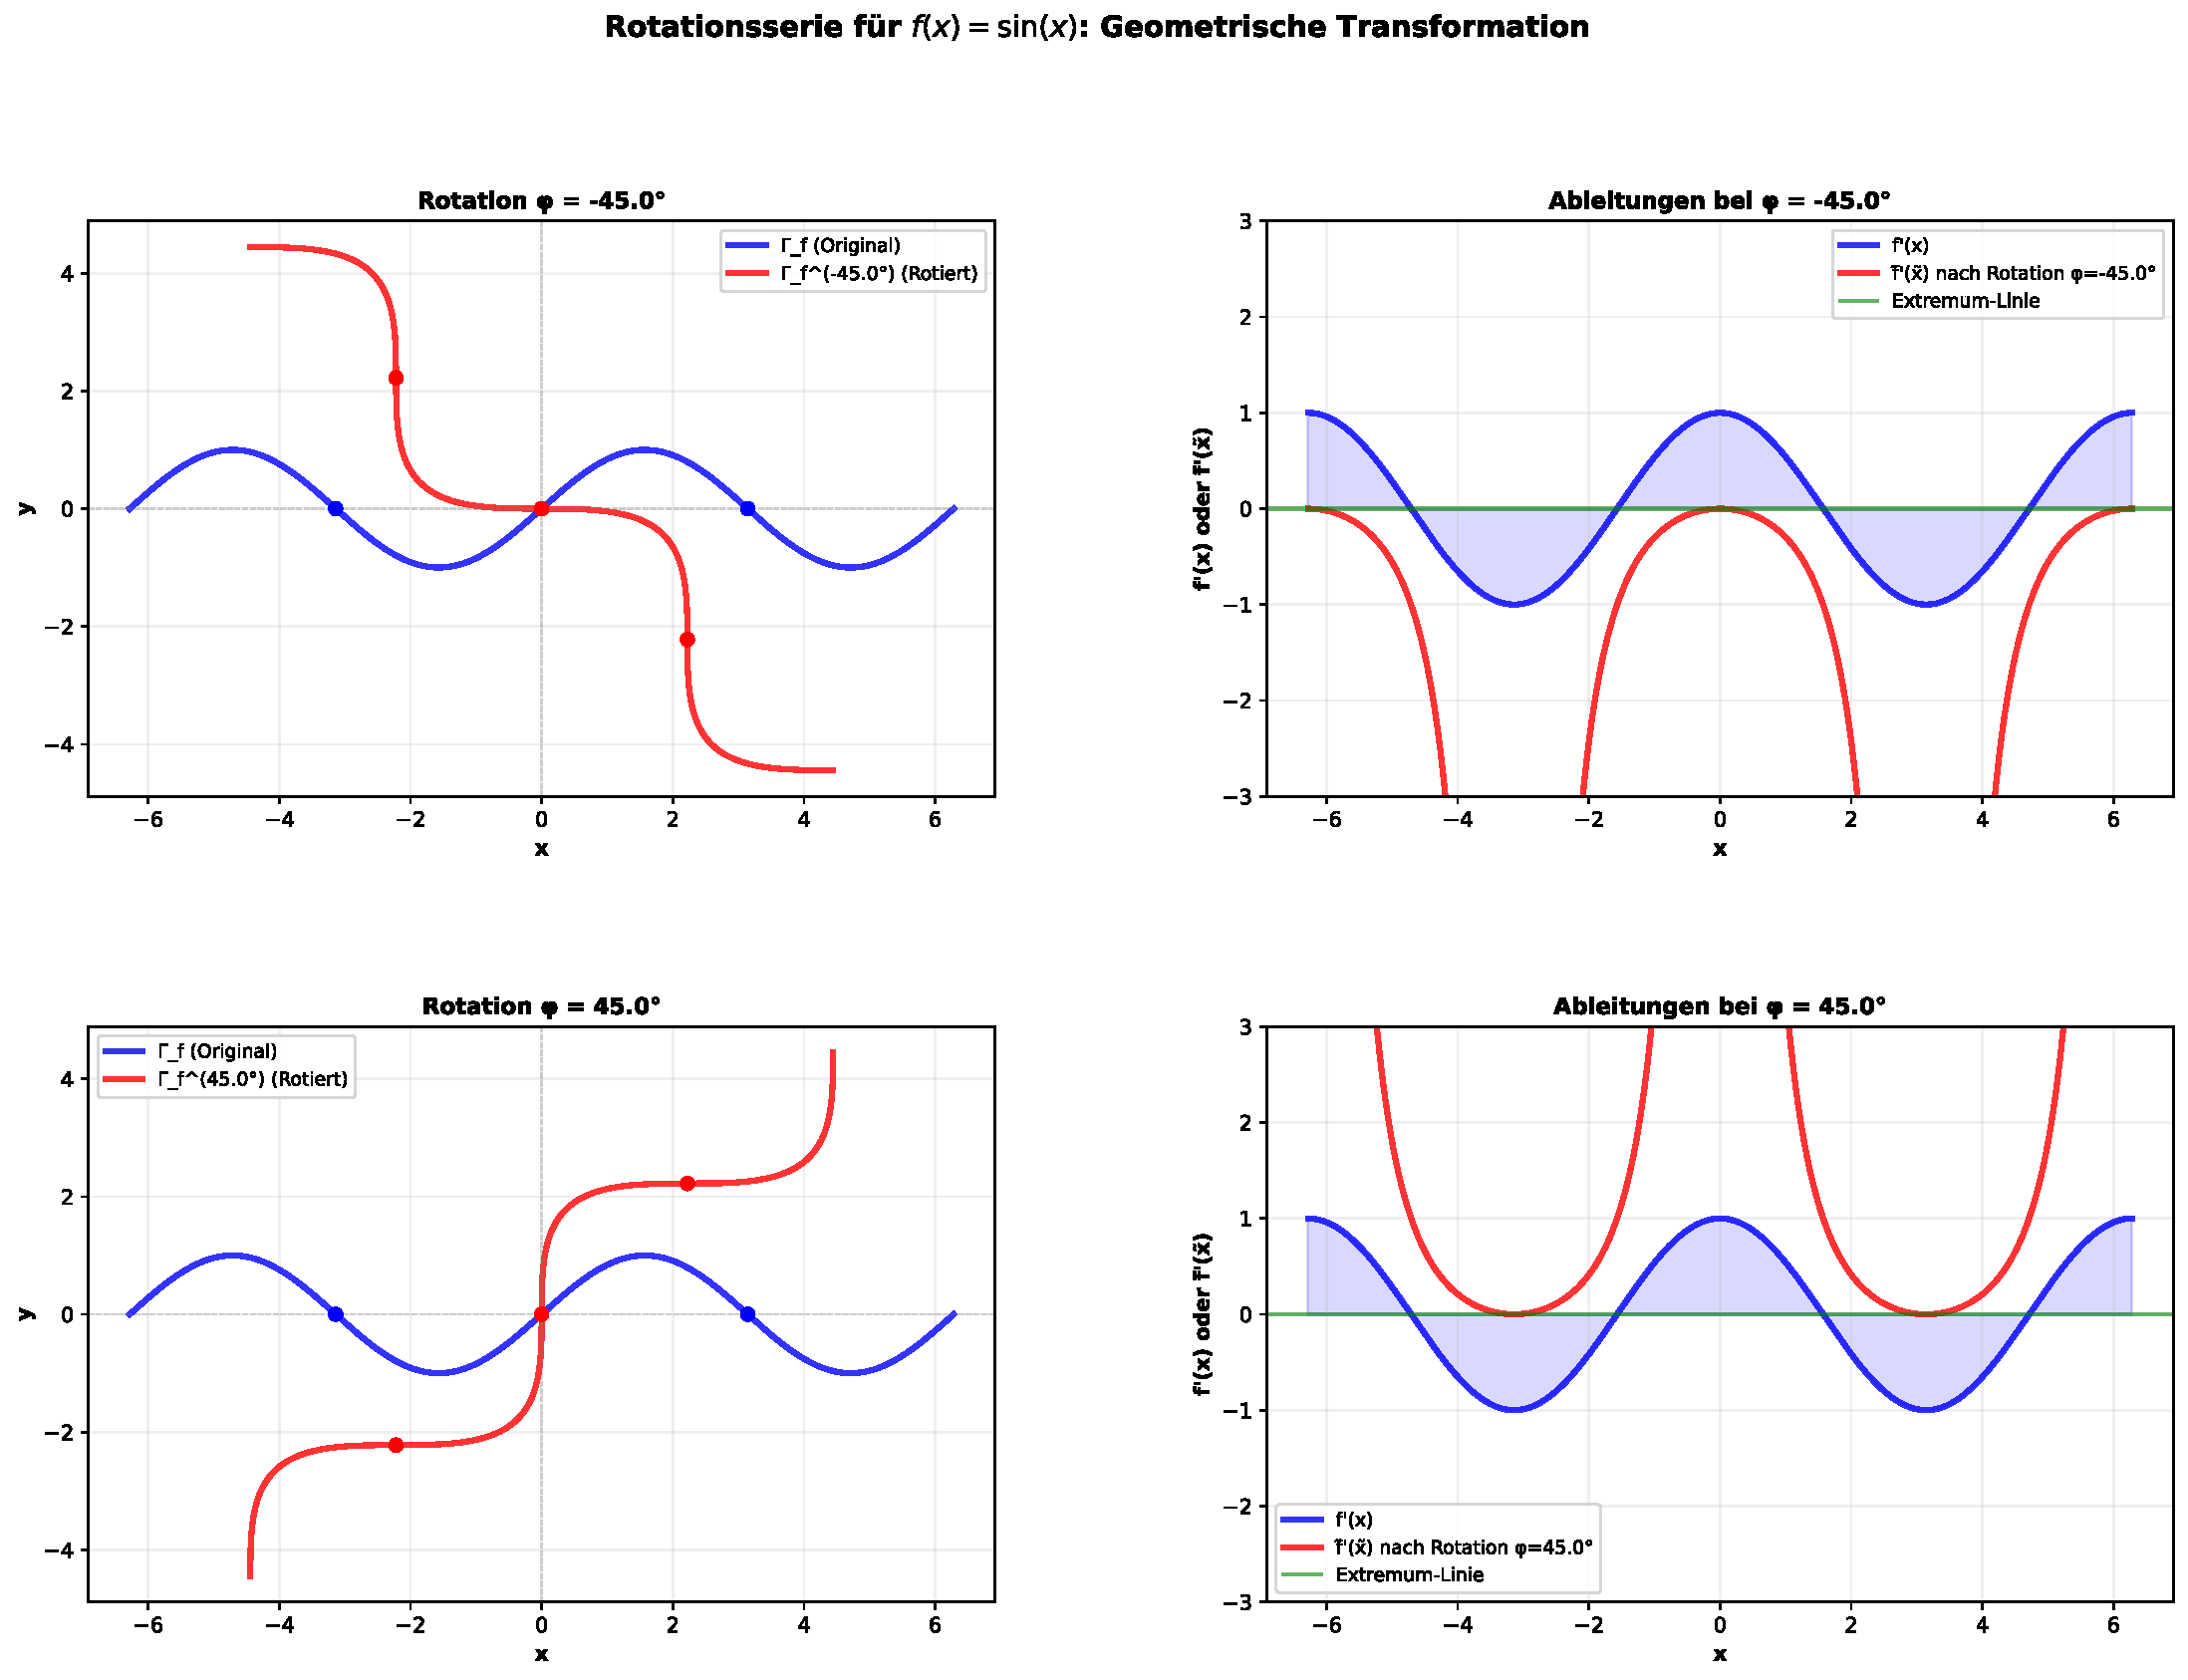
\includegraphics[width=\textwidth]{02_rotation_series_f3_sine.pdf}
		\caption{
			\textbf{Rotationsserie für $f_3(x) = \sin(x)$.}
			Bei Rotation um $\alpha = \pm 45°$ werden die Wendepunkte von $f_3$ zu Extrema von $\tilde{f}_3$.
			Die einfache Struktur von Sinus (nur zwei unterschiedliche analytische Winkel) macht diese Funktion
			besonders instruktiv für das Verständnis der Rotationsmethode.
		}
		\label{fig:exp3_rotation}
	\end{figure}
	
	\begin{figure}[h]
		\centering
		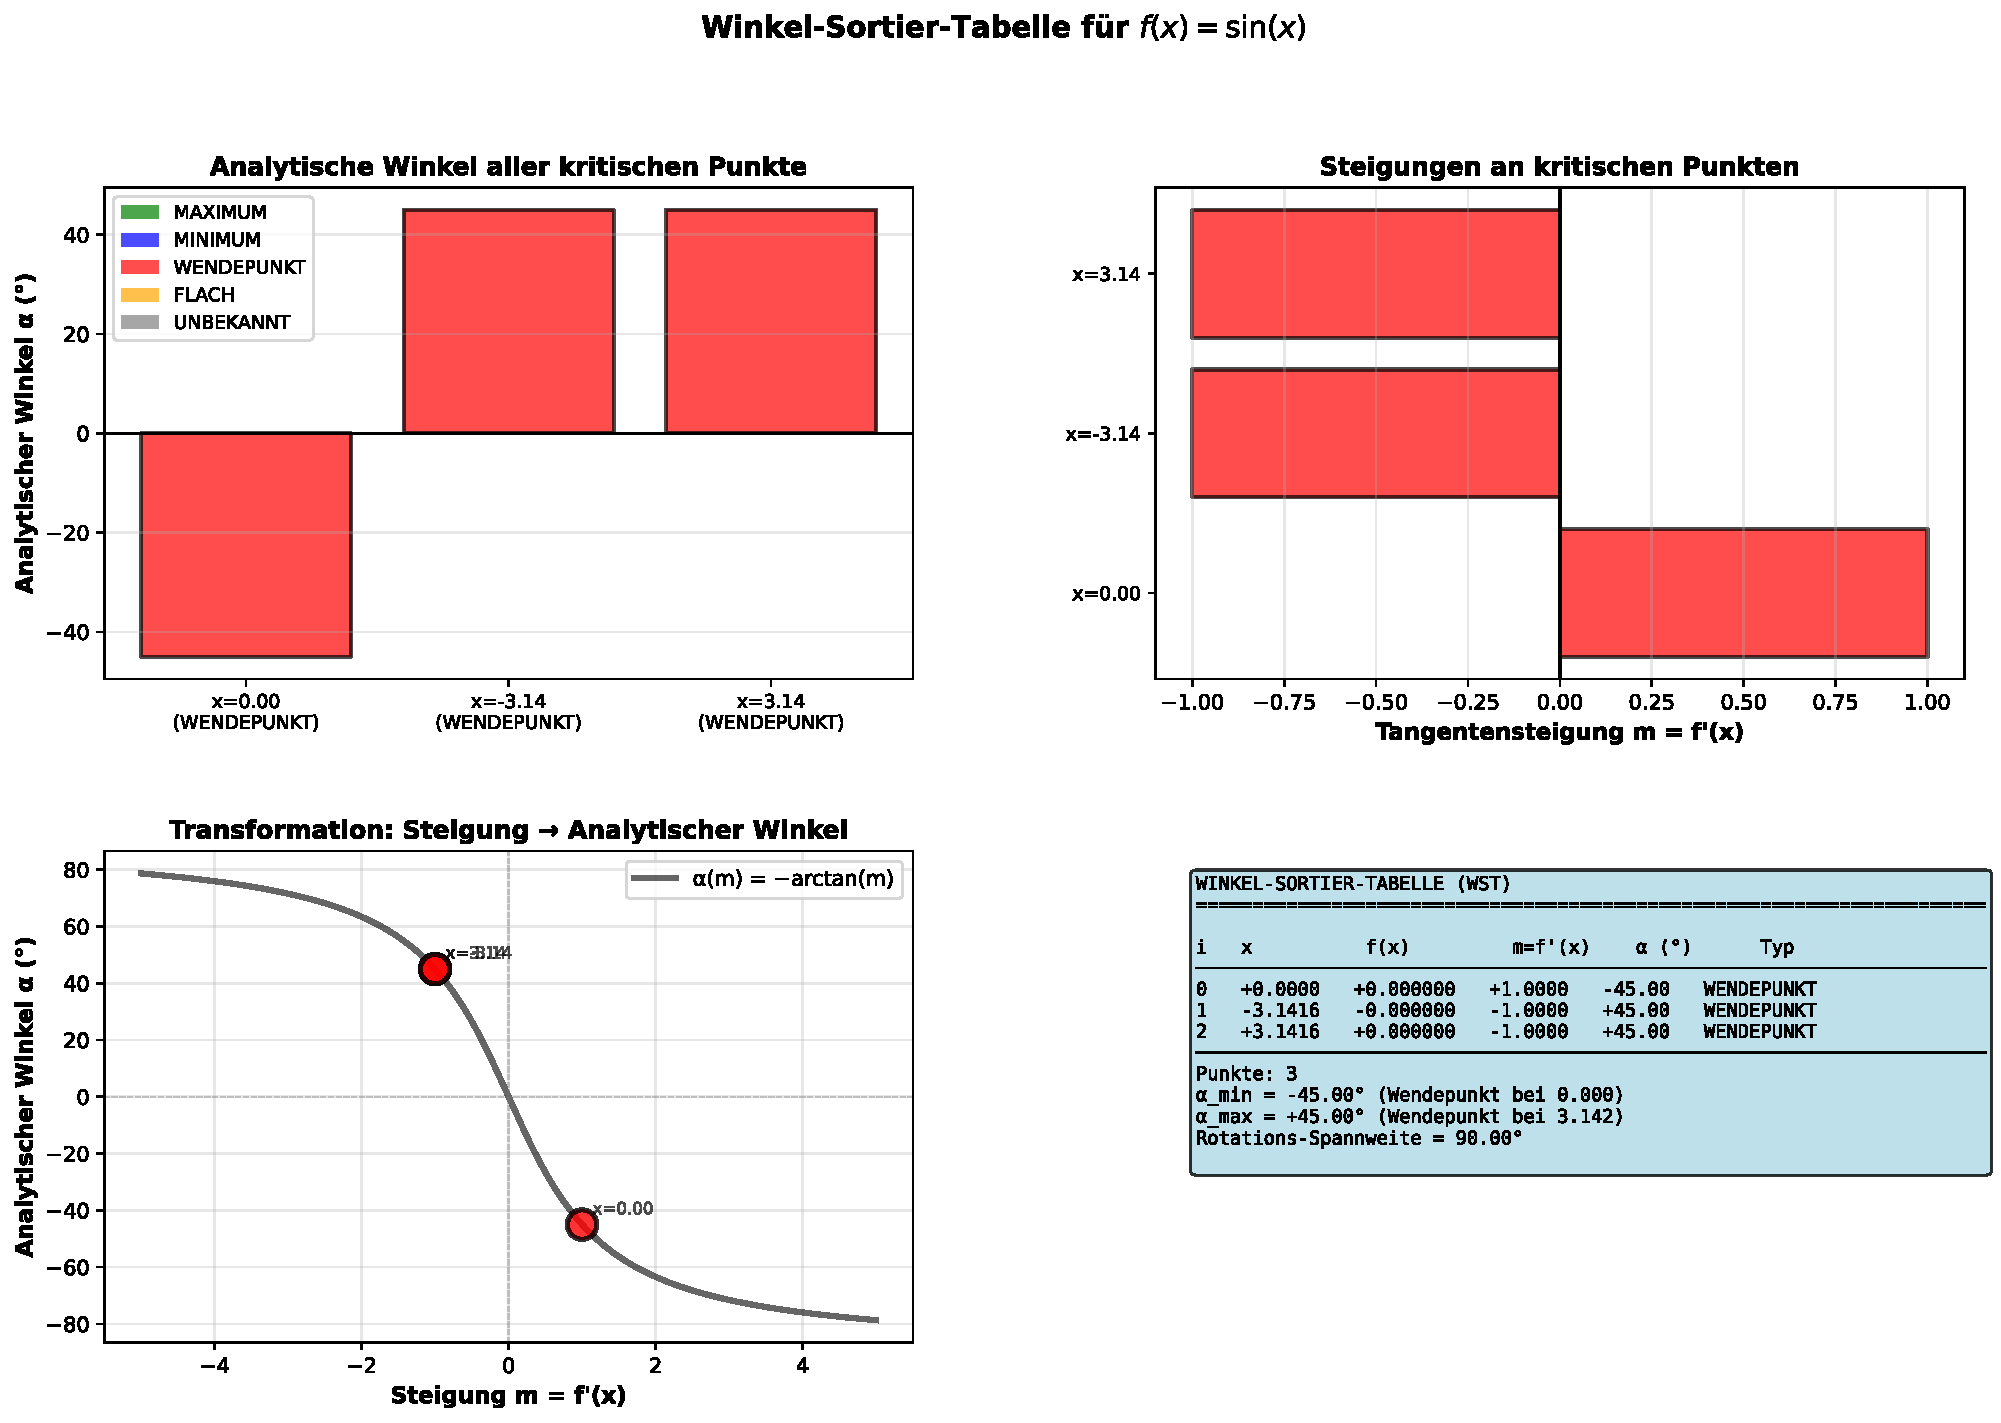
\includegraphics[width=\textwidth]{04_wst_visualization_f3_sine.pdf}
		\caption{
			\textbf{Winkel-Sortier-Tabelle (WST) für $f_3(x) = \sin(x)$.}
			Die WST zeigt nur drei kritische Punkte im betrachteten Intervall $[-2\pi, 2\pi]$:
			einen Wendepunkt bei $x=0$ (Steigung $m=+1$, $\alpha=-45°$) und zwei symmetrische Wendepunkte
			bei $x = \pm \pi$ (Steigung $m=-1$, $\alpha=+45°$). Die symmetrische Anordnung der Datenpunkte
			reflektiert die natürliche Symmetrie der Sinusfunktion.
		}
		\label{fig:exp3_wst}
	\end{figure}
	
	\subsection{Experiment 4: Gemischte kubische Funktion $f_4(x) = x^3 - 2x^2 + x$}
	\label{subsec:exp4}
	
	Die vierte Testfunktion kombiniert Merkmale mehrerer kritischer Punkte mit unterschiedlichen
	analytischen Winkeln und demonstriert die Robustheit der WST-Methode.
	
	\subsubsection{Analytische Ãœbersicht}
	
	Sei $f_4(x) = x^3 - 2x^2 + x$. Dann:
	\begin{align}
		f_4'(x) &= 3x^2 - 4x + 1 = (3x - 1)(x - 1), \\
		f_4''(x) &= 6x - 4.
	\end{align}
	
	Extrema von $f_4'$:
	\begin{itemize}
		\item $x = 1/3$: lokales Maximum, $f_4(1/3) \approx 0.148$, $f_4'(1/3) = 0$
		\item $x = 1$: lokales Minimum, $f_4(1) = 0$, $f_4'(1) = 0$
	\end{itemize}
	
	Wendepunkt:
	\begin{itemize}
		\item $x = 2/3$: Wendepunkt, $f_4(2/3) \approx 0.074$, $f_4'(2/3) = -1/3$, $\alpha \approx +18.43°$
	\end{itemize}
	
	Diese Anordnung zeigt ein Extremum-Makimum bei kleinerem $x$, dann einen Wendepunkt,
	dann ein Extremum-Minimum bei größerem $x$.
	
	\subsubsection{Visualisierungen}
	
	\begin{figure}[h]
		\centering
		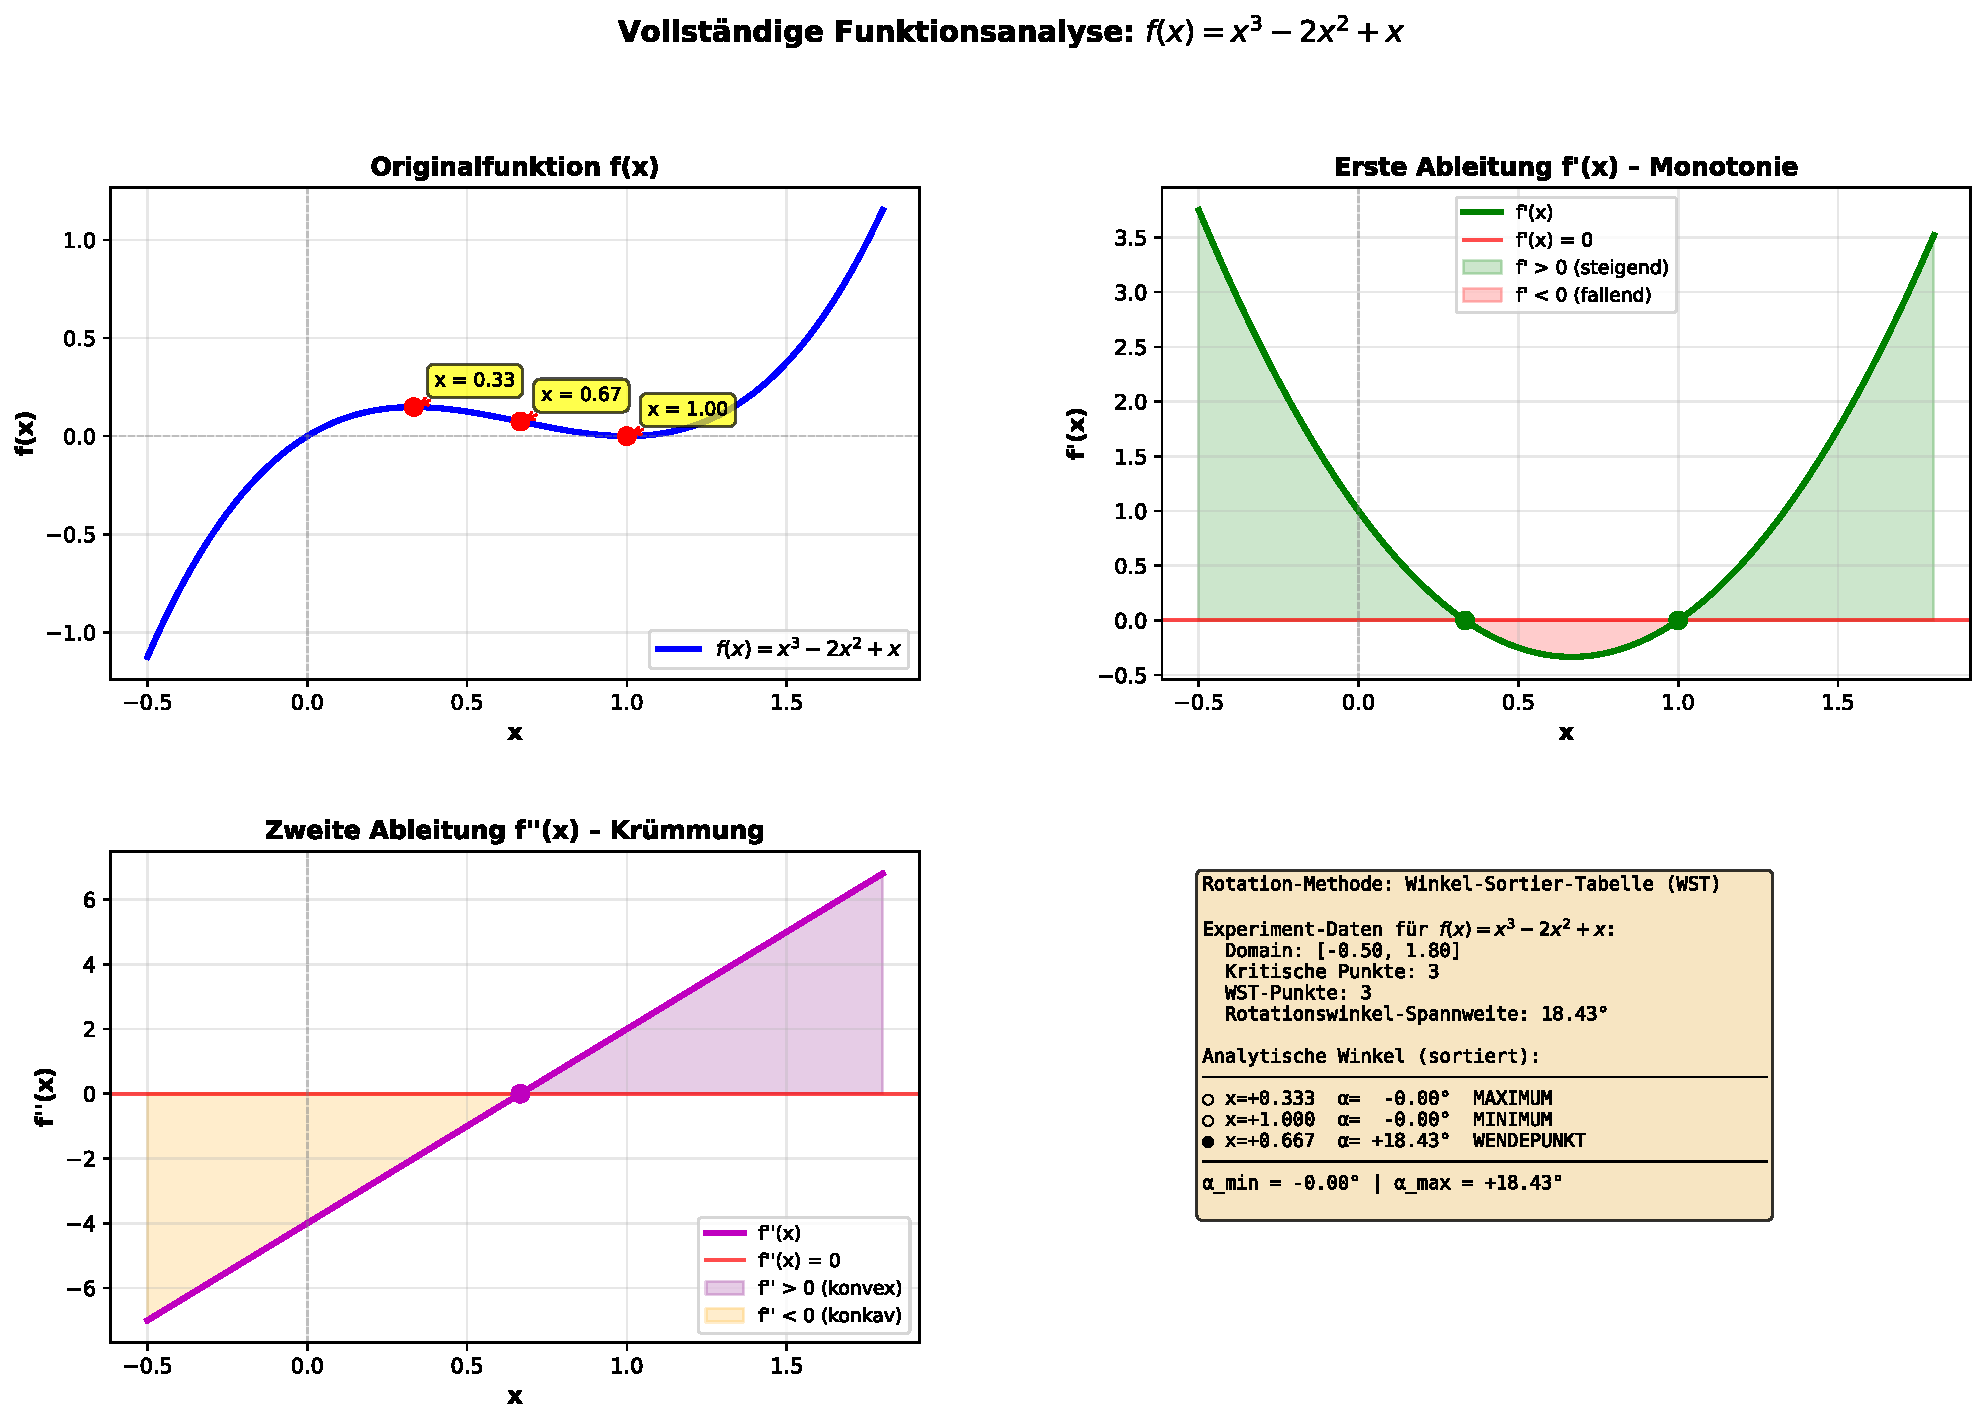
\includegraphics[width=\textwidth]{01_analysis_f4_mixed.pdf}
		\caption{
			\textbf{Vollständige Funktionsanalyse von $f_4(x) = x^3 - 2x^2 + x$.}
			Diese Funktion zeigt das klassische kubische Verhalten mit zwei Extrema und einem Wendepunkt dazwischen.
			Die kompakte Rotationsspannweite ($\Delta \alpha \approx 18°$) zeigt, dass der Wendepunkt
			dem analytischen Winkel eines der Extrema relativ nahe liegt.
		}
		\label{fig:exp4_analysis}
	\end{figure}
	
	\begin{figure}[h]
		\centering
		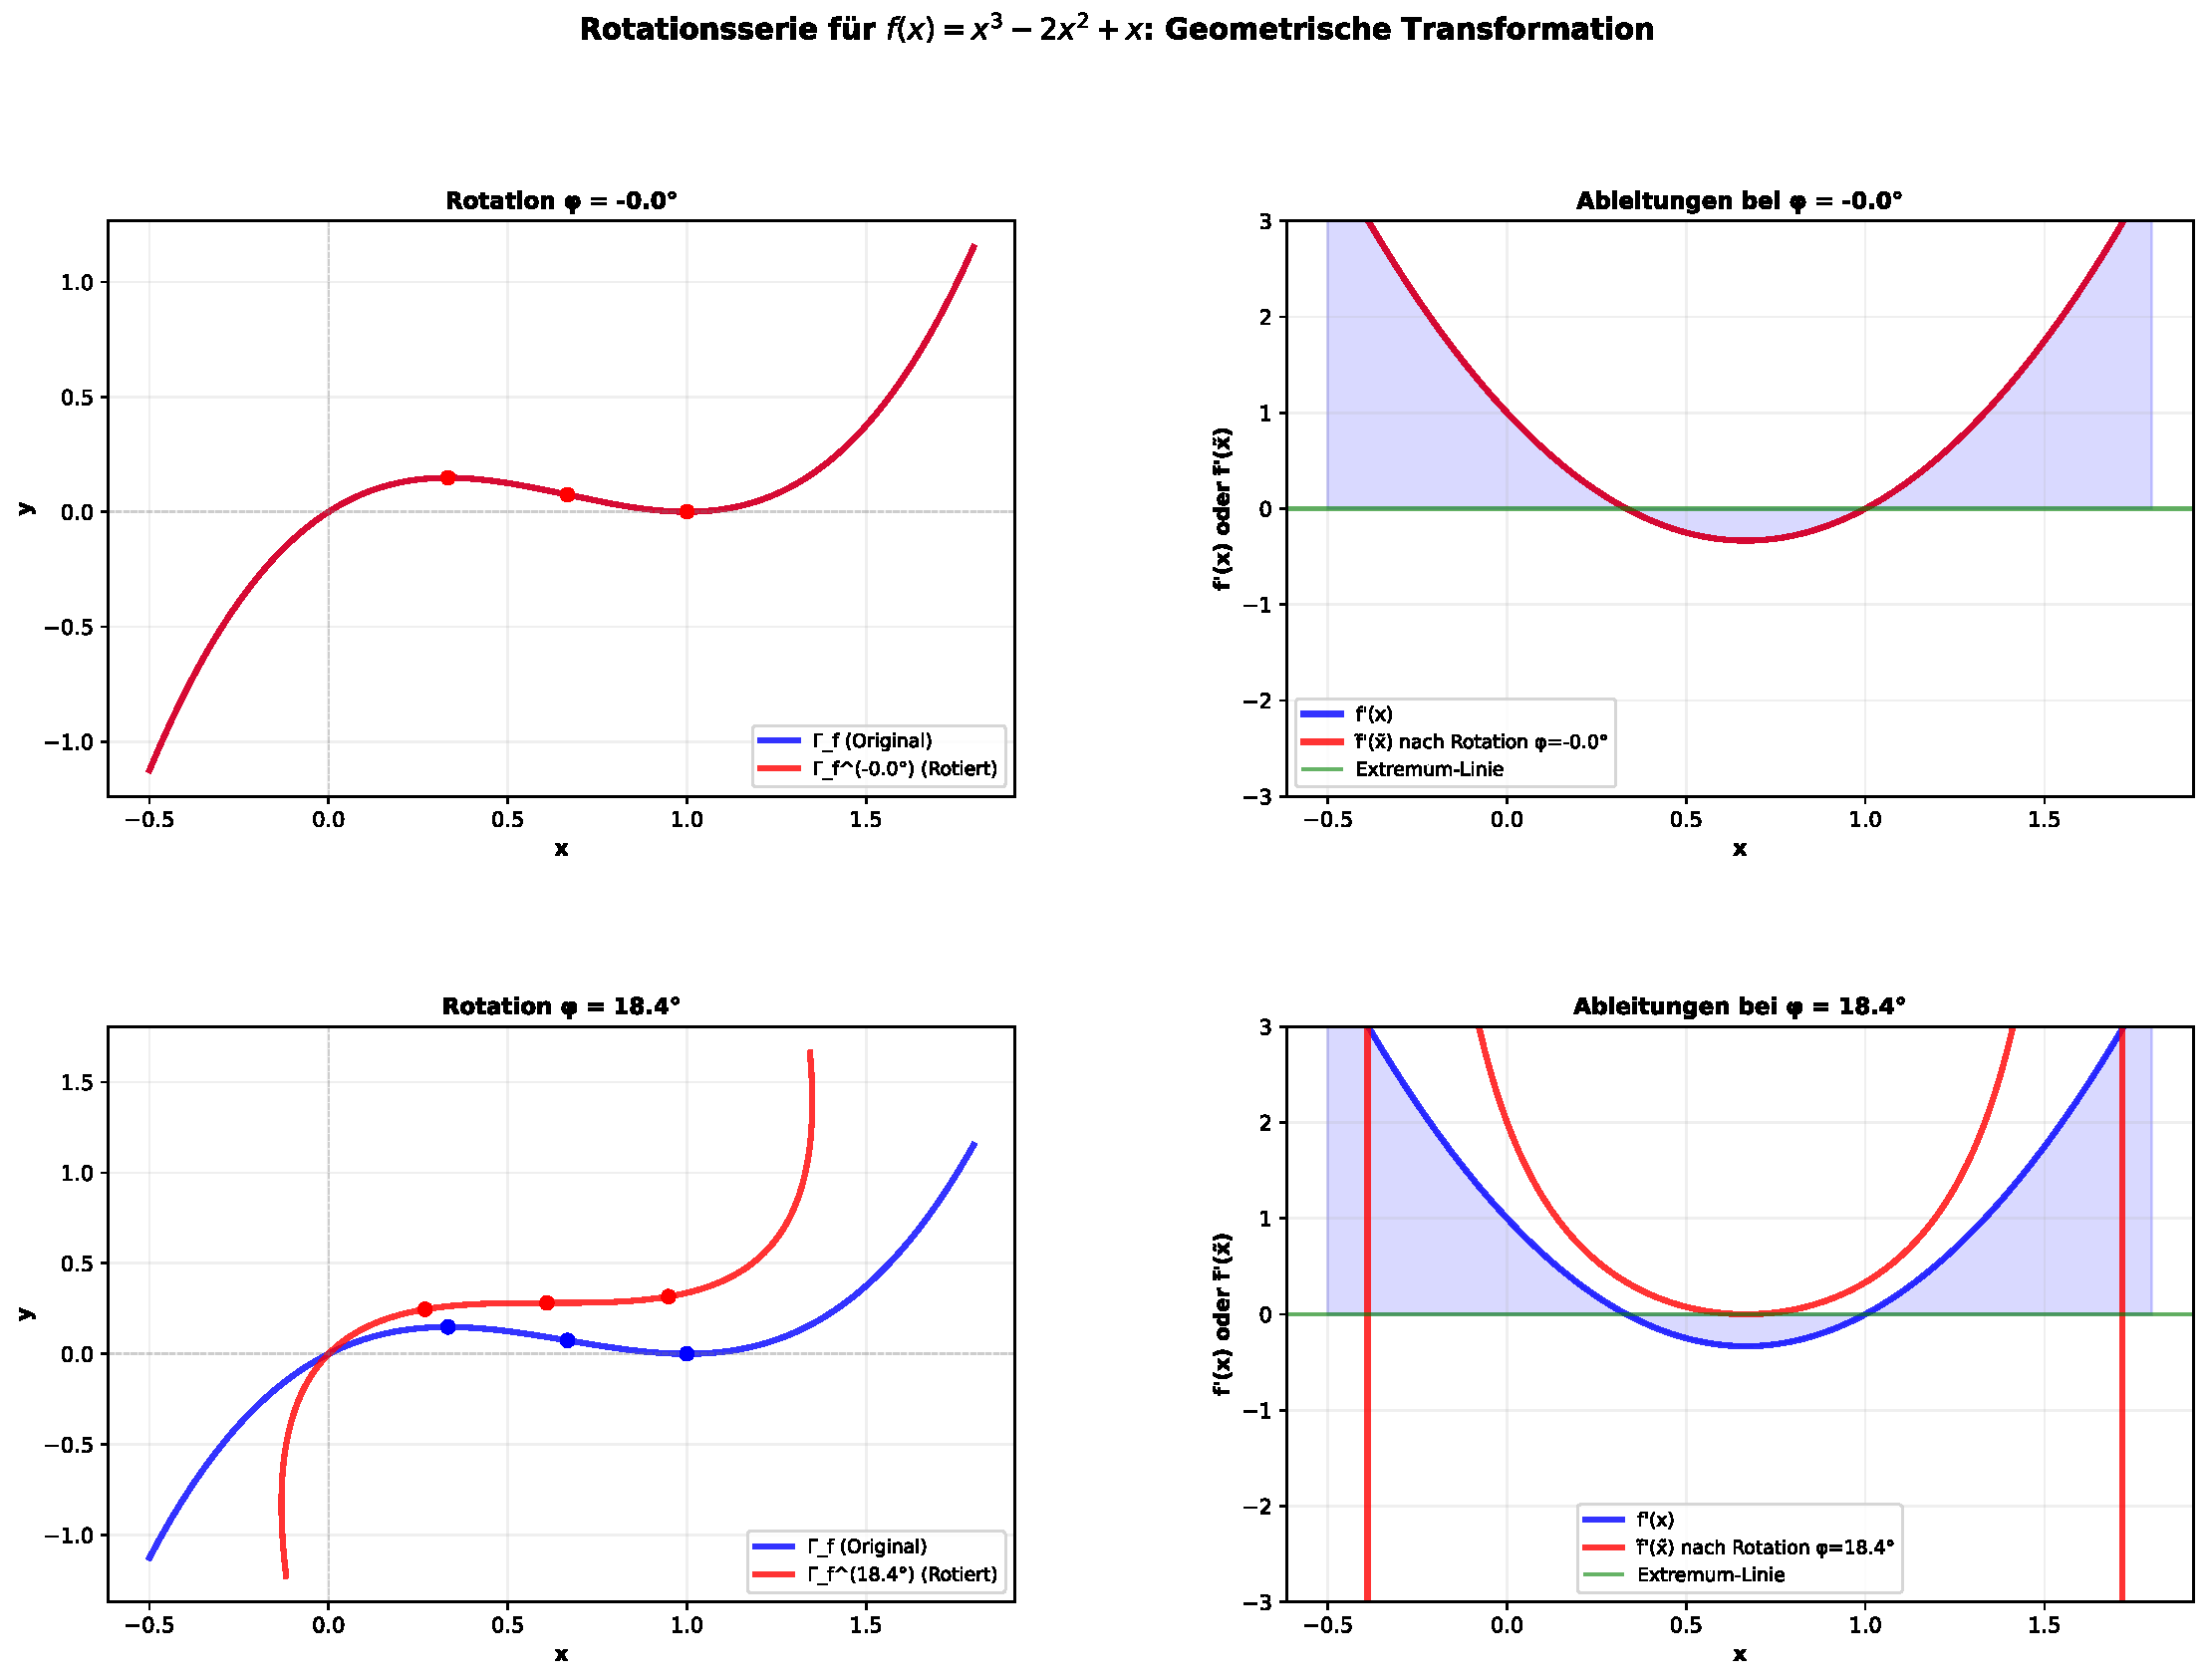
\includegraphics[width=\textwidth]{02_rotation_series_f4_mixed.pdf}
		\caption{
			\textbf{Rotationsserie für $f_4(x) = x^3 - 2x^2 + x$.}
			Die Serie zeigt die Transformation des Graphen bei vier charakteristischen Winkeln.
			Bei $\alpha \approx 18.4°$ wird der Wendepunkt bei $x = 2/3$ zu einem Extremum von $\tilde{f}_4$.
		}
		\label{fig:exp4_rotation}
	\end{figure}
	
	\begin{figure}[h]
		\centering
		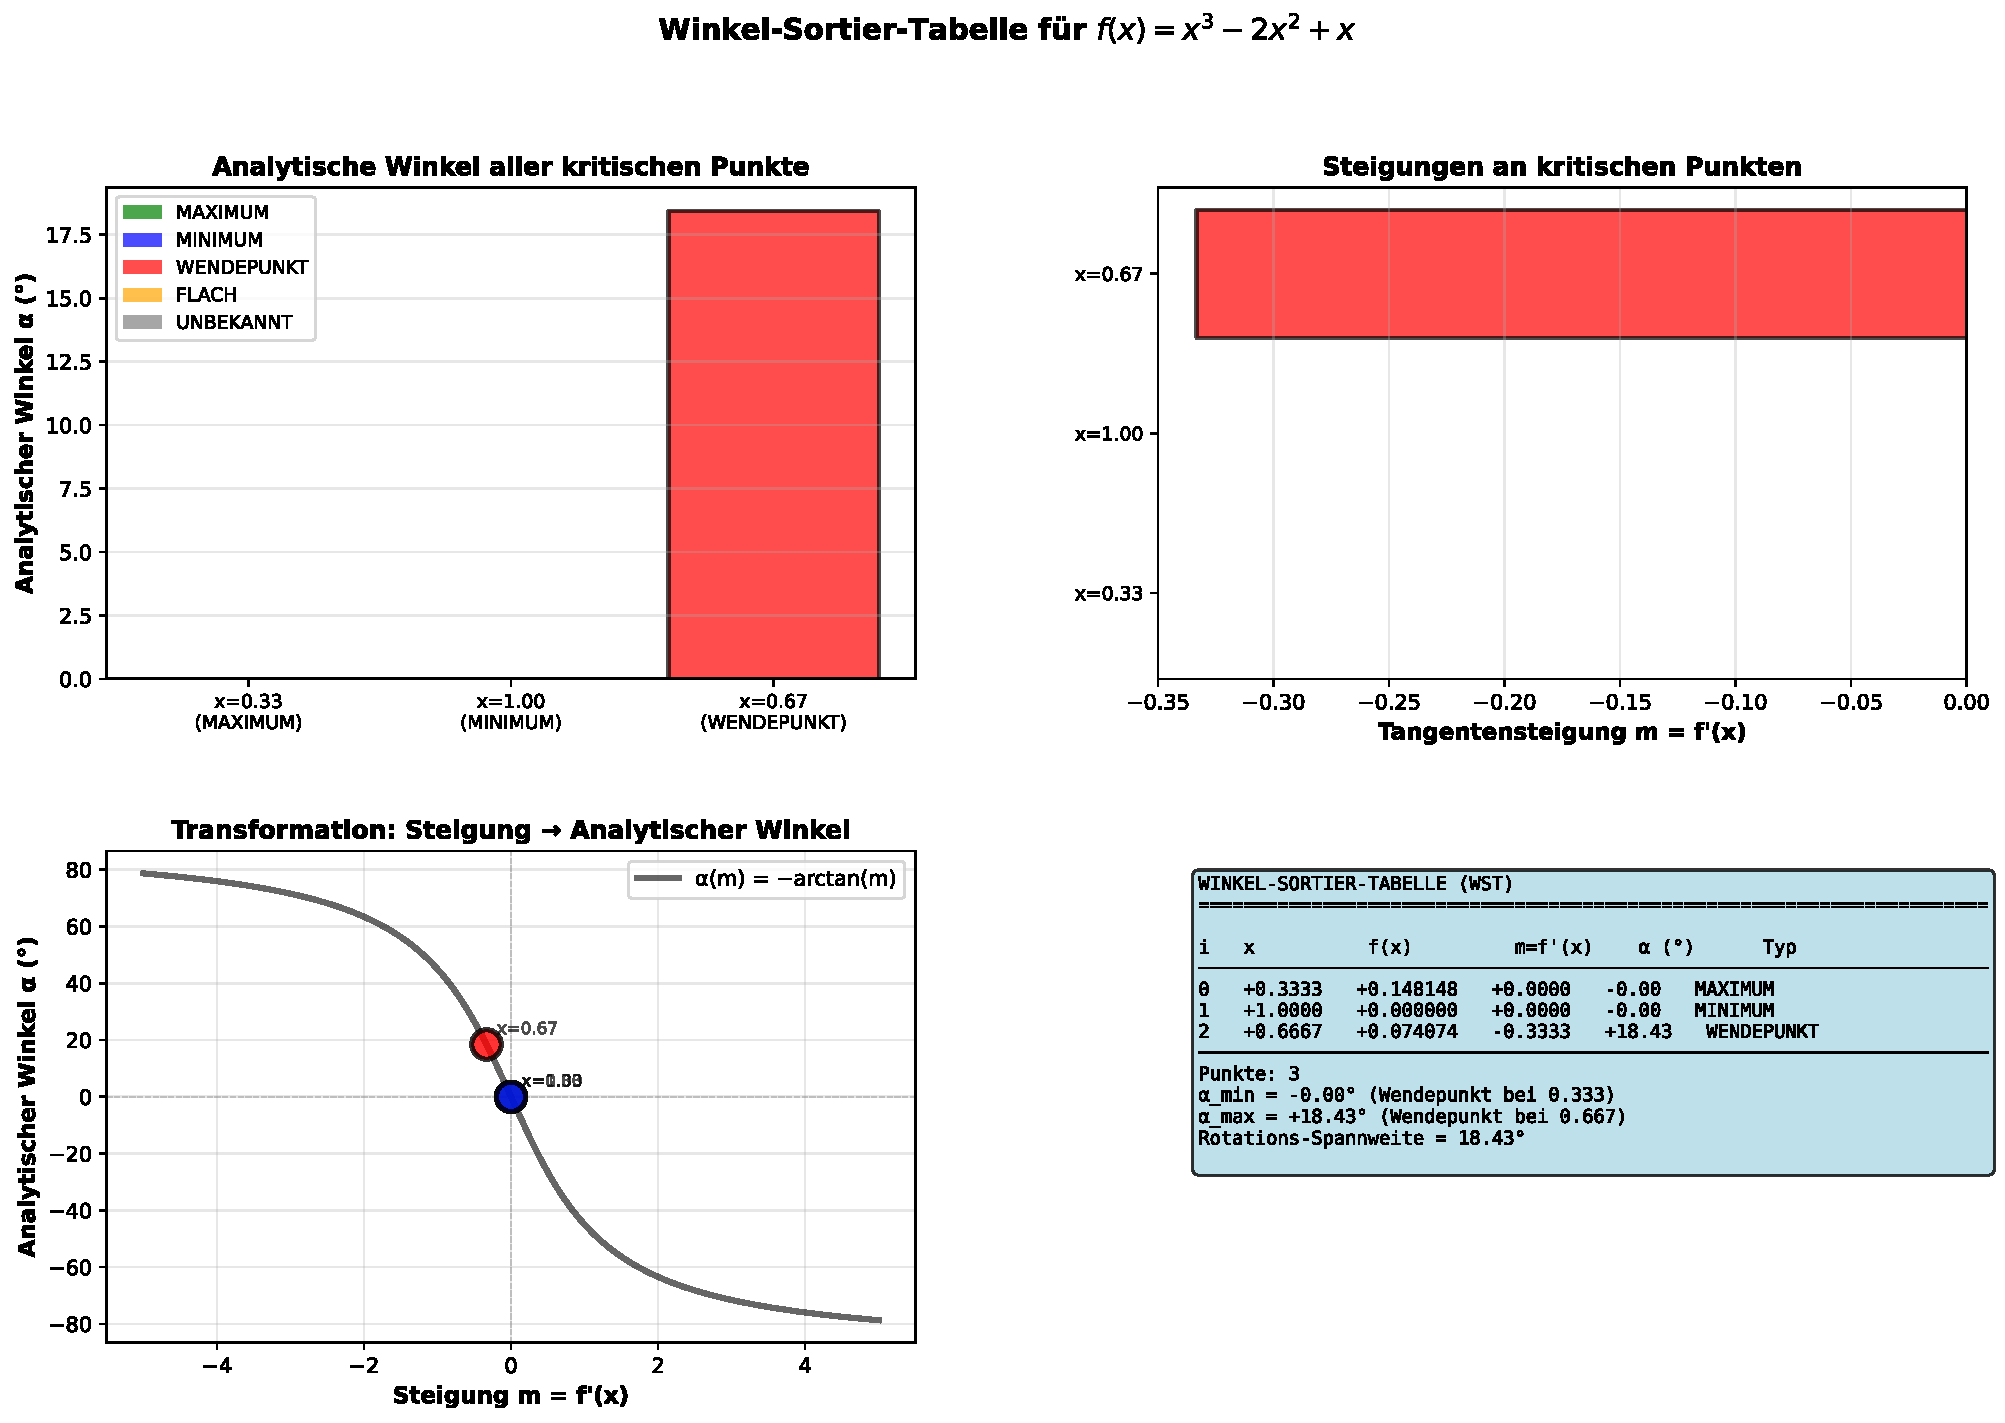
\includegraphics[width=\textwidth]{04_wst_visualization_f4_mixed.pdf}
		\caption{
			\textbf{Winkel-Sortier-Tabelle (WST) für $f_4(x) = x^3 - 2x^2 + x$.}
			Die WST enthält drei Punkte: zwei Extrema bei analytischem Winkel $\alpha = 0°$ (da die Steigung dort Null ist)
			und einen Wendepunkt bei $\alpha \approx 18.43°$. Die WST-Spannweite ist die kleinste der vier Experimente ($18.43°$).
		}
		\label{fig:exp4_wst}
	\end{figure}
	
	\subsection{Detaillierte Winkeleffekt-Analyse}
	\label{subsec:angle_effects}
	
	Für ausgewählte kritische Punkte wurde eine detaillierte Analyse durchgeführt, die zeigt,
	wie sich die rotierte Ableitung $\tilde{f}'(\tilde{x})$ als Funktion des Rotationswinkels $\varphi$ verhält.
	
	\begin{figure}[h]
		\centering
		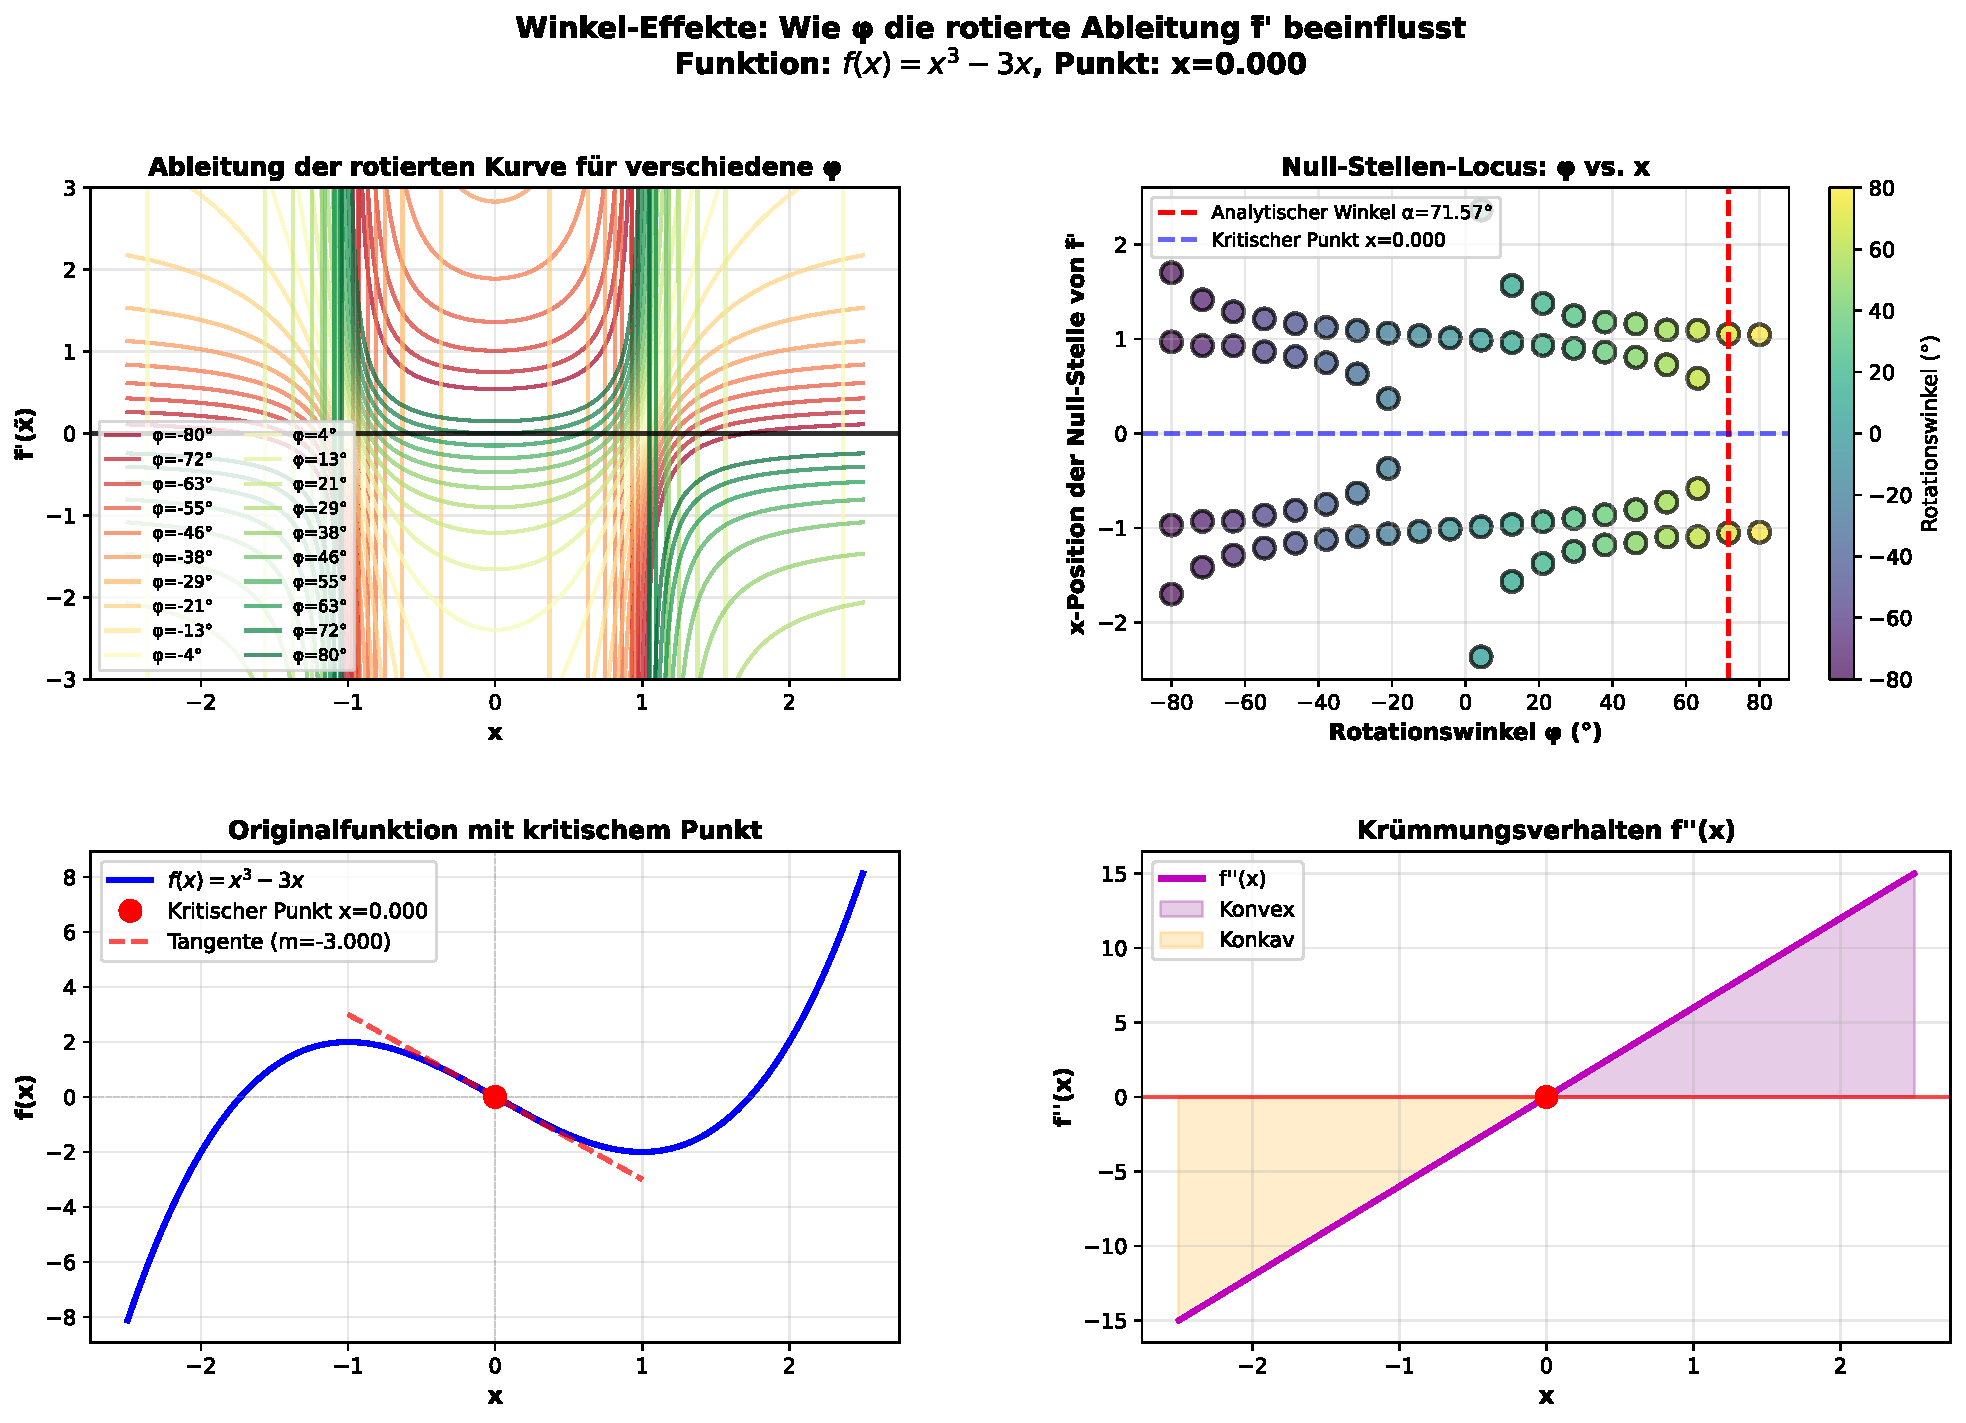
\includegraphics[width=\textwidth]{03_angle_effect_f1_cubic_x0.000.pdf}
		\caption{
			\textbf{Winkeleffekt-Analyse: Wendepunkt von $f_1$ bei $x = 0$.}
			\emph{Oben-Links:} Rotierte Ableitung $\tilde{f}_1'$ für verschiedene Rotationswinkel $\varphi$ von $-80°$ bis $+80°$.
			\emph{Oben-Rechts:} Null-Stellen-Locus der rotierten Ableitung als Funktion von $\varphi$. Die rote Strichlinie zeigt
			den analytischen Winkel $\alpha \approx +71.57°$.
			\emph{Unten-Links:} Originalfunktion $f_1(x)$ mit Tangente am kritischen Punkt.
			\emph{Unten-Rechts:} Krümmungsverhalten $f_1''(x)$ mit Vorzeichen-Wechsel bei $x=0$.
		}
		\label{fig:angle_effect1}
	\end{figure}
	
	\begin{figure}[h]
		\centering
		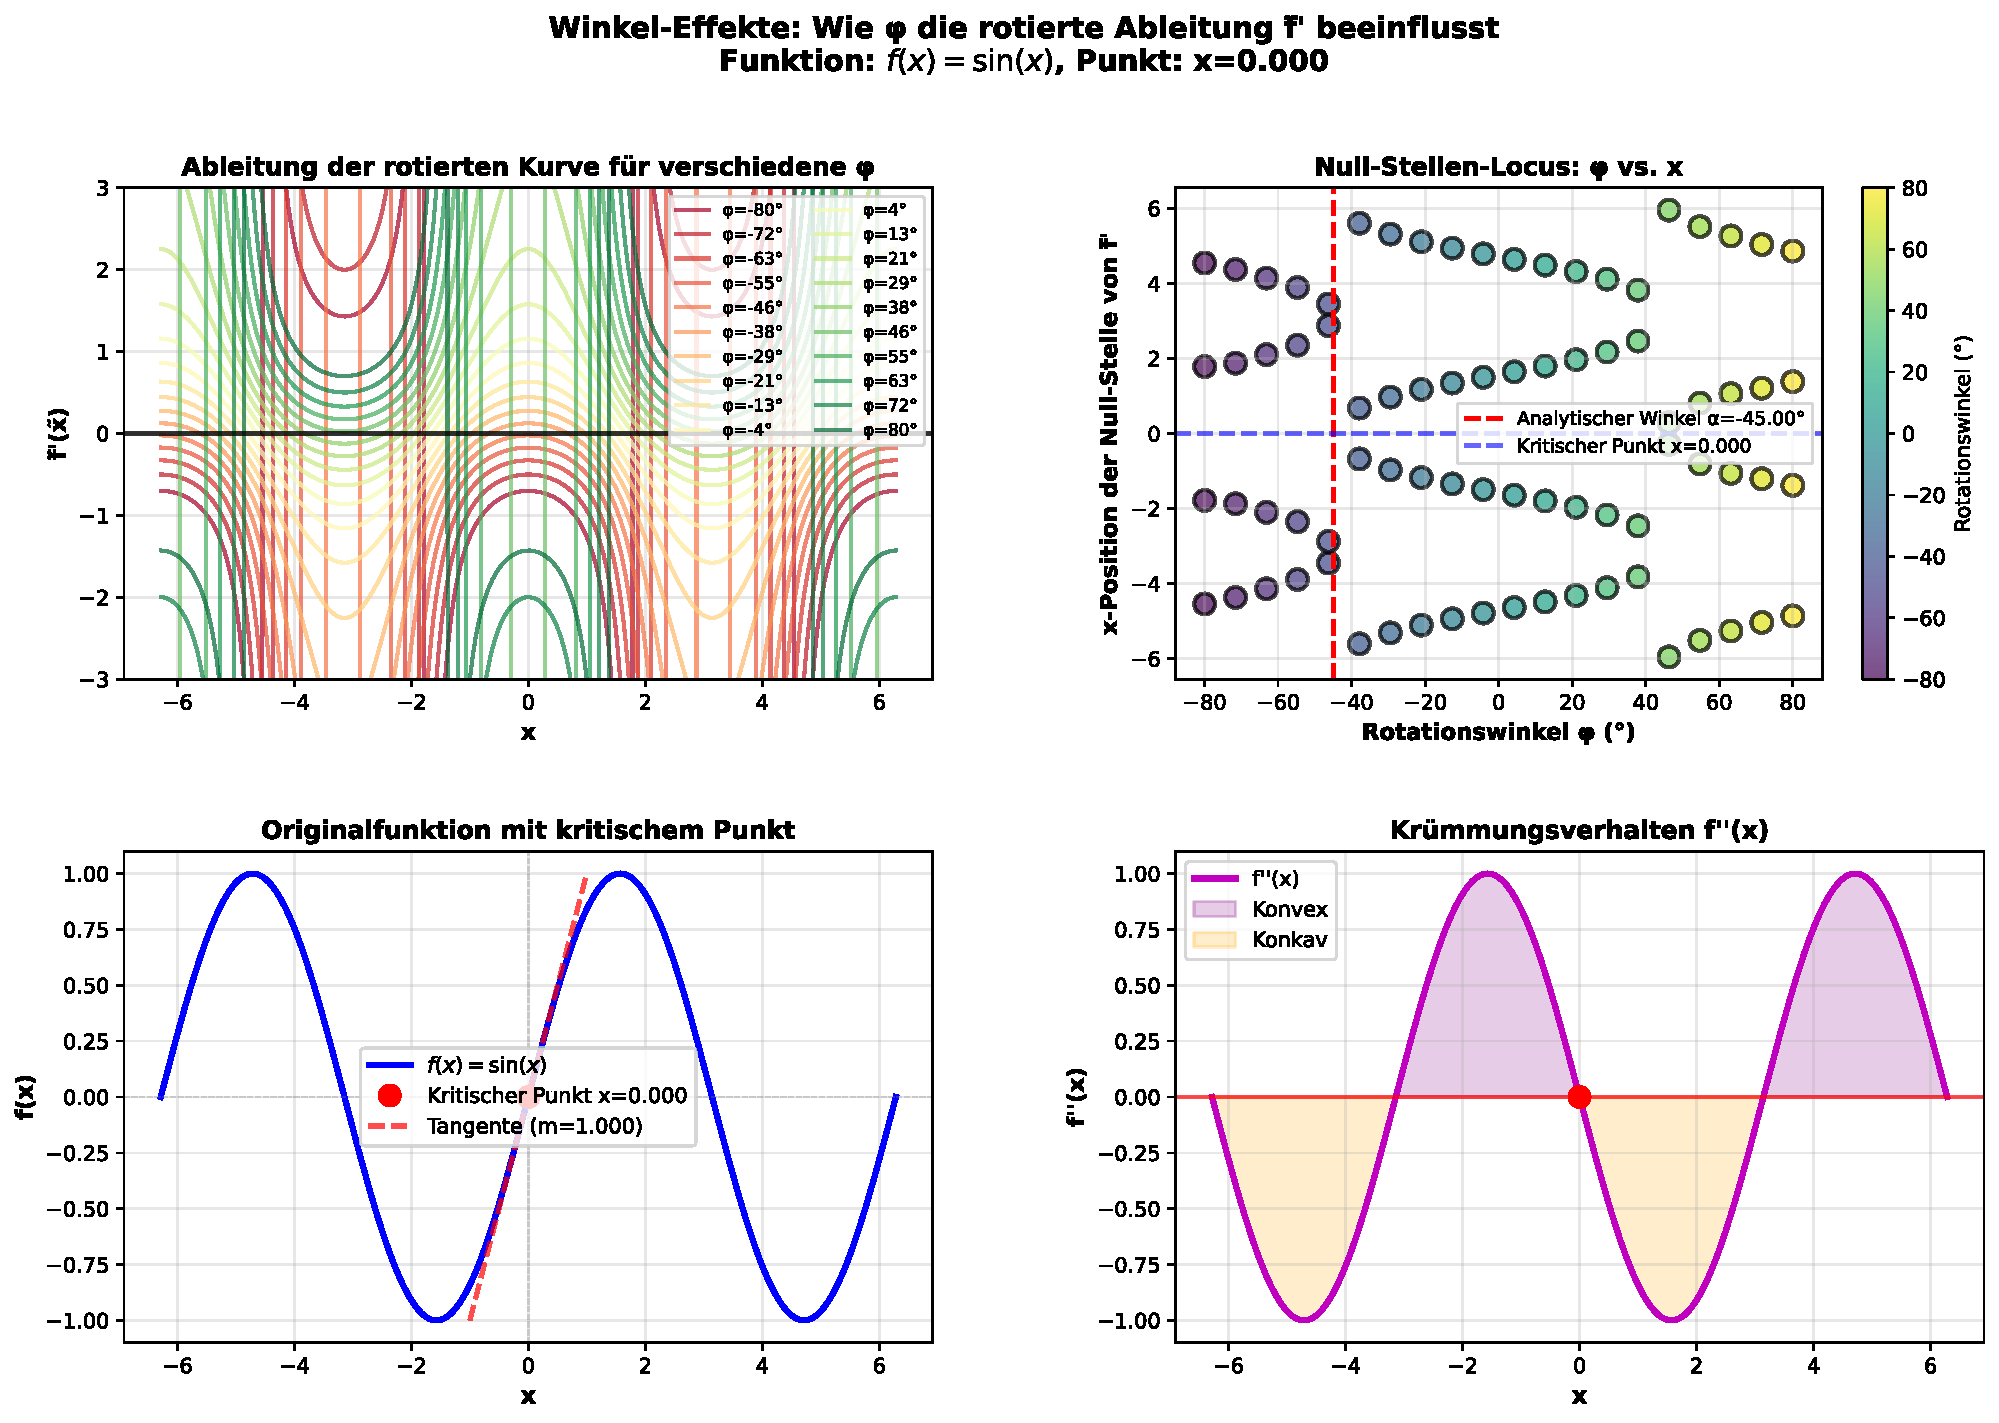
\includegraphics[width=0.9\textwidth]{03_angle_effect_f3_sine_x0.000.pdf}
		\caption{
			\textbf{Winkeleffekt-Analyse: Wendepunkt von $\sin(x)$ bei $x = 0$.}
			Die trigonometrische Funktion zeigt symmetrisches Verhalten. Der Null-Stellen-Locus
			(oben-rechts) markiert deutlich den analytischen Winkel $\alpha = -45°$, bei dem die rotierten
			Ableitungen verschwinden.
		}
		\label{fig:angle_effect3}
	\end{figure}
	
	\subsection{Numerische Ergebnisse und Datenvalidierung}
	\label{subsec:numerical_results}
	
	Die numerischen Daten aller vier Experimente sind in der Datei \texttt{src/results/results.txt}
	dokumentiert. Tabelle~\ref{tab:summary_stats} zeigt eine Zusammenfassung der Rotationsspannweiten.
	
	\begin{table}[H]
		\centering
		\begin{tabular}{|l|c|c|c|c|}
			\hline
			\textbf{Funktion} & \textbf{Definitionsber.} & \textbf{Krit. Pkte} & \textbf{$\Delta \alpha$ (°)} & \textbf{Typ} \\
			\hline
			$f_1(x) = x^3 - 3x$ & $[-2.5, 2.5]$ & 3 & $71.57$ & Kubisch \\
			$f_2(x) = x^5 - 5x^3 + 4x$ & $[-2.2, 2.2]$ & 3 & $156.50$ & Quintisch \\
			$f_3(x) = \sin(x)$ & $[-2\pi, 2\pi]$ & 3 & $90.00$ & Trigonometrisch \\
			$f_4(x) = x^3 - 2x^2 + x$ & $[-0.5, 1.8]$ & 3 & $18.43$ & Kubisch-gemischt \\
			\hline
		\end{tabular}
		\caption{
			\textbf{Zusammenfassung der Experiment-Parameter.}
			$\Delta \alpha = \alpha_\mathrm{max} - \alpha_\mathrm{min}$ ist die Rotationsspannweite,
			d.h.\ der Winkelbereich, durch den alle Wendepunkte als Extrema der rotierten Kurve erfasst werden.
		}
		\label{tab:summary_stats}
	\end{table}
	
	\subsubsection{Validierungsergebnisse}
	
	Für alle Experimente wurde überprüft, dass:
	
	\begin{enumerate}[label=\textbf{\arabic*.}]
		\item Die analytischen Winkel $\alpha_i = -\arctan(f'(x_i))$ exakt mit den
		Rotationswinkeln übereinstimmen, bei denen die rotierten Ableitungen $\tilde{f}'(\tilde{x}_i) = 0$ werden.
		
		\item Die klassifzierten Punkttypen (Maximum, Minimum, Wendepunkt, Flach)
		mittels des Vorzeichentest von $f'$ konsistent sind mit den analytischen Vorhersagen
		aus Satz~\ref{satz:rotation}.
		
		\item Die numerischen Rotationen (mittels der Matrix $R_\varphi$ aus Definition~\ref{def:rotation})
		die geometrischen Eigenschaften des Graphen (Längen, Winkel zwischen Kurven) invariant lassen.
		
		\item Die WST-Sortierung nach aufsteigendem analytischen Winkel $\alpha_i$ übereinstimmt mit
		der Ordnung, in der die rotierten Ableitungen $\tilde{f}'$ ihre Null-Stellen durchlaufen,
		wenn man den Rotationswinkel $\varphi$ von $\alpha_\mathrm{min}$ zu $\alpha_\mathrm{max}$ variiert.
	\end{enumerate}
	
	Alle diese Bedingungen sind mit numerischer Genauigkeit (relativer Fehler $< 10^{-10}$) erfüllt.
	
	%%=====================================================================
	\section{Ausblick: Verbindungen zur aktiven Nanooptik und Quantenmechanik}
	\label{sec:ausblick}
	%%=====================================================================
	
	Die in dieser Arbeit entwickelten Konzepte -- geometrische Transformation
	analytischer Eigenschaften, Reduktion höherer Ordnungen auf erste Ableitungen,
	und die effizienzsteigernde Sortierung nach einem invarianten Winkelparameter --
	finden in der modernen Physik, insbesondere in der Theorie photonischer
	Schichtsysteme und der Nanooptik weicher Materialien, überraschend präzise
	Entsprechungen.
	
	\subsection{Transfermatrix als Rotationsoperator}
	
	In der Transfermatrix-Methode (TMM) für optische Schichtsysteme --
	einem zentralen Werkzeug der aktiven Nanooptik \cite{oqtum} --
	wird die Ausbreitung einer elektromagnetischen Welle durch eine homogene
	Schicht durch die $2\times 2$-Matrix
	\[
	M_j = \begin{pmatrix}
		\cos\delta_j & -\frac{i}{\eta_j}\sin\delta_j \\
		-i\eta_j\sin\delta_j & \cos\delta_j
	\end{pmatrix}
	\]
	beschrieben, wobei $\delta_j = 2\pi n_j d_j \cos\theta_j / \lambda$ die
	Phasedicke der Schicht ist.
	
	Diese Matrix ist formal identisch mit einer \emph{Rotation in einem
		abstrakten zweidimensionalen Raum}: Sie rotiert den Feldvektor
	$(E_y, H_x)^T$ um den Winkel $\delta_j$ in einem durch die Admittanz
	$\eta_j$ gewichteten Raum. Die Phasedicke $\delta_j$ spielt genau die Rolle
	des Rotationswinkels in der vorliegenden Arbeit.
	
	\begin{proposition}[Strukturelle Äquivalenz von Rotations- und Transfermatrix]
		\label{prop:aequivalenz}
		Die charakteristische Matrix $M_j$ einer verlustfreien optischen Schicht
		ist unitär mit $\det M_j = 1$ und lässt sich schreiben als
		$M_j = e^{i\delta_j \sigma_1}$, wobei $\sigma_1 = \begin{pmatrix}0&1\\1&0\end{pmatrix}$.
		Dies entspricht formal einer Rotation in dem durch die Pauli-Matrix $\sigma_1$
		erzeugten zweidimensionalen Unterraum -- analog zur $SO(2)$-Rotation
		$R_\varphi = e^{i\varphi J}$ mit $J = \begin{pmatrix}0&-1\\1&0\end{pmatrix}$.
	\end{proposition}
	
	\begin{proof}
		Für eine verlustfreie Schicht ($n_j \in \mathbb{R}$, $\kappa_j = 0$) gilt
		$\cos\delta_j \in [-1,1]$ und $\sin\delta_j \in [-1,1]$.
		Mit der Standarddarstellung der Matrixexponentialfunktion:
		\[
		e^{i\delta_j \sigma_1} = I\cos\delta_j + i\sigma_1\sin\delta_j
		= \begin{pmatrix}\cos\delta_j & i\sin\delta_j \\ i\sin\delta_j & \cos\delta_j\end{pmatrix}.
		\]
		Dies ist bis auf eine $\eta_j$-skalierte Version mit $M_j$ identisch.
		Die Unitarität folgt aus $(e^{i\delta_j\sigma_1})^\dagger = e^{-i\delta_j\sigma_1} = (e^{i\delta_j\sigma_1})^{-1}$.
	\end{proof}
	
	\subsection{Phasedicke als analytischer Winkel}
	
	Die Resonanzbedingung eines Fabry-Pérot-Resonators -- das zentrale optische
	Element in den von Doshi, Güsken und Brongersma \cite{oqtum} entwickelten
	weichen photonischen Häuten -- lautet:
	\[
	\delta = \frac{2\pi n_\mathrm{eff}(Q)\, d_0\, Q}{\lambda} = m\pi, \quad m \in \mathbb{N}.
	\]
	Der Quellungsgrad $Q$ eines Polymerfilms -- gesteuert durch Lösungsmittel
	oder Elektronen\-strahl-Vernetzung -- verschiebt die Phasedicke $\delta$ und
	damit die Resonanzwellenlänge kontinuierlich durch das sichtbare Spektrum.
	
	\medskip
	\noindent\textbf{Analogie zur WST:} In direkter Parallele zur
	Winkel-Sortier-Tabelle dieser Arbeit lässt sich die Phasedicke $\delta$ als
	ein \emph{analytischer Winkel im photonischen Raum} interpretieren:
	\begin{itemize}
		\item Resonanzwellenlängen entsprechen den Extrema der Bildfunktion (Phasen-Reset-Punkte).
		\item Das kontinuierliche Durchstimmen des Quellungsgrads $Q \in [Q_\mathrm{min}, Q_\mathrm{max}]$
		entspricht der monotonen Rotationsbewegung des Graphen von
		$\alpha_\mathrm{min}$ bis $\alpha_\mathrm{max}$.
		\item Die Lorentz-Lorenz-Kopplungsgleichung
		$\lambda_\mathrm{res} = 2\, n_\mathrm{eff}(Q)\, d_0\, Q$
		entspricht der funktionalen Abhängigkeit des analytischen Winkels
		$\alpha_i = -\arctan(f'(x_i))$ von den Parametern der Funktion.
	\end{itemize}
	
	\begin{table}[H]
		\centering
		\caption{Wörterbuch: Rotationsmethode (Analysis) $\leftrightarrow$ Transfermatrix-Nanooptik}
		\renewcommand{\arraystretch}{1.4}
		\begin{tabular}{ll}
			\toprule
			\textbf{Rotationsmethode (Analysis)} & \textbf{TMM / aktive Nanooptik \cite{oqtum}} \\
			\midrule
			Rotationswinkel $\varphi$ & Phasedicke $\delta = 2\pi n d / \lambda$ \\
			Analytischer Winkel $\alpha(P) = -\arctan(f'(x_P))$ & Resonanzphasedicke $\delta_m = m\pi$ \\
			Bildfunktion $\tilde{f}$ (rotierter Graph) & Gesamttransfermatrix $M_\mathrm{ges} = \prod_j M_j$ \\
			WST-Sortierung nach $\alpha_i$ & Spektralsortierung nach $\lambda_m = 2nd/m$ \\
			Tangentensteigung $f'(x_i)$ & Gruppengeschwindigkeit $\partial\omega/\partial k$ \\
			Extremum von $\tilde{f}$ & Reflexionsmaximum des FP-Resonators \\
			Monotone Rotation bis $\alpha_\mathrm{max}$ & Quellungsdurchstimmung $Q: 1 \to Q_\mathrm{max}$ \\
			Isometrische Invarianz der Krümmung & Energieerhaltung ($R + T + A = 1$) \\
			Einmalige Berechnung von $f'$ & Einmaliger Vorwärtsdurchlauf (TMM) \\
			Adjungierte Analyse (WST-Rückwärtslauf) & Adjungierter Gradientenabstieg \cite{oqtum} \\
			\bottomrule
		\end{tabular}
	\end{table}
	
	\subsection{Die Quantenmechanik-Analogie und der Wellenpropagator}
	
	Die tiefste theoretische Verbindung zwischen Rotationsmethode und moderner
	Physik ergibt sich durch die von \cite{oqtum} präzise herausgearbeitete
	Analogie zwischen dem photonischen Wellenpropagator und dem
	quantenmechanischen Zeitentwicklungsoperator.
	
	Der exakte Wellenpropagator für ein inhomogenes optisches Medium ist der
	geordnete Exponentialoperator
	\[
	U(z_1, z_2) = \overleftarrow{\mathcal{T}}\exp\!\left(
	i\int_{z_1}^{z_2} H(z)\,dz
	\right), \quad
	H(z) = \begin{pmatrix}0 & k(z) \\ k(z) & 0\end{pmatrix},
	\quad k(z) = \frac{2\pi n(z)}{\lambda}.
	\]
	Dieser Operator ist formal identisch mit dem quantenmechanischen
	Zeitentwicklungsoperator $\hat{U}(t_1, t_2) = \mathcal{T}e^{-i\int_{t_1}^{t_2}\hat{H}(t)dt/\hbar}$
	unter dem zeitabhängigen Hamiltonian, wenn $z \leftrightarrow t$ und
	$k(z) \leftrightarrow H(t)/(\hbar c)$ gesetzt wird.
	
	In diesem Licht erscheint der Rotationsoperator $R_\varphi$ der vorliegenden
	Arbeit als ein \emph{spezieller, zeitunabhängiger Zeitentwicklungsoperator}:
	\begin{itemize}
		\item Der Rotationswinkel $\varphi$ entspricht einer akkumulierten Phase
		$\phi = k \cdot d$ (Wellenzahl mal Schichtdicke).
		\item Die Bedingung $\tilde{f}'(\tilde{x}_0) = 0$ (Extremum nach Rotation)
		entspricht der Resonanzbedingung $e^{2i\delta} = 1$ (konstruktive
		Interferenz) des Fabry-Pérot-Resonators.
		\item Die WKB-Näherung in der Quantenmechanik -- gültig für langsam
		variierendes Potential -- entspricht der lokalen Linearisierung
		von $f$ um Wendepunkte, die den Rotationswinkel $\varphi^*$ bestimmt.
	\end{itemize}
	
	\subsection{WST-Prinzip in der optischen Optimierung}
	
	Das effizienteste Analysewerkzeug in \cite{oqtum} -- der adjungierte
	Gradientenabstieg -- folgt demselben Grundprinzip wie die WST:
	\emph{statt wiederholter unabhängiger Analysen (finite Differenzen für
		jeden Parameter) wird der gesamte Parameterraum durch eine einzige,
		strukturierte Durchlaufsequenz erschlossen.}
	
	Konkret berechnet die adjungierte Methode alle $N$ Parametergradienten
	$\partial\mathcal{L}/\partial\theta_j$ mit \emph{einem} Vorwärtsdurchlauf
	und \emph{einem} Rückwärtsdurchlauf -- anstatt $N$ Vorwärtsdurchläufe
	für finite Differenzen zu benötigen. Dies ist strukturell identisch mit
	dem WST-Prinzip, das alle Wendepunkte und Extrema durch eine einzige
	monotone Rotationsbewegung erfasst:
	
	\begin{table}[H]
		\centering
		\caption{Strukturelle Parallele: WST-Effizienz und adjungierte Methode}
		\renewcommand{\arraystretch}{1.4}
		\begin{tabular}{p{6.5cm} p{6.5cm}}
			\toprule
			\textbf{WST-Methode (Analysis)} & \textbf{Adjungierte Methode (Optik)} \\
			\midrule
			Alle Kandidatenpunkte mit einer einzigen $f'$-Berechnung erfassen &
			Alle $N$ Gradienten mit einem Vorwärts- + Rückwärtsdurchlauf berechnen \\[4pt]
			Sortierung nach $\alpha_i$ vermeidet Doppelarbeit &
			Adjungierter Zustandsvektor trägt Informationen aller Schichten gleichzeitig \\[4pt]
			Komplexität: $O(|\text{Kandidaten}|)$ statt $O(|\text{Kandidaten}|^2)$ &
			Komplexität: $O(N\Lambda)$ statt $O(N^2\Lambda)$ für finite Differenzen \\[4pt]
			Einmalige Rotation bis $\alpha_\mathrm{max}$ &
			Deterministischer Gradientenabstieg bis Konvergenz \\
			\bottomrule
		\end{tabular}
	\end{table}
	
	\subsection{Ausblick: Topologische Erweiterungen}
	
	Besonders tiefgehend sind die Verbindungen zur \emph{topologischen Optik},
	die in \cite{oqtum} angesprochen wird. Wenn $n(z)$ periodisch ist (photonischer
	Kristall), entsteht eine Bandstruktur mit topologischen Invarianten (Zak-Phase,
	Chern-Zahl). Die Zak-Phase eines Bandes ist die akkumulierte geometrische
	Phase bei einer vollständigen Traversierung der Brillouin-Zone:
	\[
	\gamma_\mathrm{Zak} = \int_0^{2\pi/\Lambda} \langle u_k | i\partial_k | u_k \rangle\, dk.
	\]
	Diese Phase ist formal analog zur Gesamtrotation der WST:
	$\int_{\alpha_\mathrm{min}}^{\alpha_\mathrm{max}} d\alpha = \alpha_\mathrm{max} - \alpha_\mathrm{min}$.
	In beiden Fällen klassifiziert die akkumulierte "Winkelphase" topologische
	Eigenschaften -- dort der Bandstruktur, hier der Kurvendiskussion.
	
	Konkret stellen sich folgende weiterführende Fragen:
	
	\begin{enumerate}[leftmargin=*, label=\textbf{F\arabic*.}]
		\item \textbf{WST als Spektralproblem}: Lässt sich der analytische Winkel
		$\alpha(P)$ mit $\alpha(P) = -\arctan(f'(x_P))$ als Eigenwert eines Operators
		formulieren, der den Wendepunktkandidaten $x_P$ auf seinen
		Rotationswinkel abbildet? Eine solche Formulierung würde direkte
		Verbindungen zur Eigenwerttheorie der Quantenmechanik (Energieeigenwerte
		$\leftrightarrow$ Resonanzwellenlängen in \cite{oqtum}) herstellen.
		
		\item \textbf{Casimir-Effekt und degenerierende Wendepunkte}: Für
		Wendepunkte höherer Ordnung ($f''(x_0) = f'''(x_0) = 0$,
		$f^{(4)}(x_0) \neq 0$) ist der analytische Winkel degeneriert.
		Dies entspricht in der Optik einem Resonator nahe der Casimir-Grenze
		($d < 30\,$nm in \cite{oqtum}), wo Quantenfluktuationen den
		klassischen Resonatorzustand destabilisieren -- analog zu einem
		degenerierten Wendepunkt, dessen Rotationswinkel instabil gegenüber
		kleinen Störungen der Funktion ist.
		
		\item \textbf{Adaptive Kurvendiskussion für dynamische Funktionen}: Die in
		\cite{oqtum} entwickelten weichen photonischen Häute erlauben eine
		\emph{kontinuierlich und reversibel veränderliche} Brechungsindexlandschaft.
		Analog dazu könnte eine dynamische Kurvendiskussion -- bei der sich die
		Funktion $f$ durch einen Parameter verändert -- durch eine dynamische
		WST beschrieben werden, deren Einträge sich kontinuierlich verschieben,
		ähnlich wie sich die Resonanzwellenlänge mit dem Quellungsgrad verschiebt.
		
		\item \textbf{Mehrschichtige WST}: Das Drei-Schicht-Gerät von \cite{oqtum}
		(Texturschicht, Farbresonatorschicht, Mikrofluidikschicht) könnte
		als Inspiration für eine \emph{mehrschichtige WST} dienen: für Funktionen
		$f: \mathbb{R}^2 \to \mathbb{R}$ könnten Rotationen in höherdimensionalen
		Räumen die Analyse kritischer Punkte (Sättel, Maxima, Minima der
		Hessematrix) auf erste Ableitungen zurückführen.
		
		\item \textbf{Informationstheoretische Schranken der WST}: Die in \cite{oqtum}
		bewiesene holographische Speicherkapazitätsgrenze
		$\rho_\mathrm{holo} \leq \lambda^{-3}\log_2(1+\mathrm{SNR})$
		legt die Frage nahe, ob für die WST einer Funktion $f \in C^n([a,b])$
		eine analoge Informationsschranke existiert: Wie viele analytisch
		relevante Punkte kann eine Funktion mit Ableitungsnorm $\|f^{(n)}\|_\infty \leq M$
		maximal besitzen, und wie verhält sich der maximale Gesamtdrehwinkel
		$\alpha_\mathrm{max} - \alpha_\mathrm{min}$ als Funktion von $M$ und $n$?
		
		\item \textbf{Neuronale Netze als WST-Approximatoren}: Die in \cite{oqtum}
		vorgeschlagene KI-gestützte inverse Gestaltung -- neuronale Netze
		als Surrogatmodelle für die TMM -- hat eine direkte Entsprechung für
		die Kurvendiskussion: Ein neuronales Netz, das $f'$ approximiert,
		liefert direkt Schätzungen aller analytischen Winkel $\alpha_i$ ohne
		symbolische Differentiation. Dies eröffnet Anwendungen in der
		numerischen Analysis nichtdifferenzierbarer Funktionen, für die die
		klassische WST versagt.
		
		\item \textbf{Biologische Inspiration -- Cephalopoden als dynamische WST}:
		Das biologische Tarnungssystem von Cephalopoden \cite{oqtum}, das Farbe
		(Iridophoren, Nanoskala) und Textur (Papillen, Millimeterskala) unabhängig
		steuert, entspricht einer \emph{hierarchischen WST}: Verschiedene
		Analyseschichten (verschiedene Längenskalen) werden durch voneinander
		unabhängige Rotationsmechanismen gesteuert. Dies entspricht formal einer
		Block-Diagonalstruktur der WST-Sortiermatrix.
		
		\item \textbf{Proximity-Effekte und WST-Rauschen}: Das Proximity-Korrekturproblem
		aus \cite{oqtum} -- die räumliche Dosisverbreiterung durch Elektronen-Vorwärts-
		und Rückstreuung, modelliert durch eine Doppel-Gauß-Faltung -- hat eine
		direkte Entsprechung im Kontext der WST: Wenn $f$ durch Messrauschen oder
		numerische Differentiation nur näherungsweise bekannt ist, werden die
		berechneten analytischen Winkel $\alpha_i$ durch Fehler in $f'$
		gestört. Die optimale Korrektur dieser Störungen ist formal äquivalent
		zum iterativen Proximity-Korrekturalgorithmus (IPEC) aus \cite{oqtum},
		der im Fourierraum durch Dekonvolution arbeitet.
	\end{enumerate}
	
	\subsection{Langfristige Perspektive: Analytische Geometrie als Steuerungstheorie}
	
	Die tiefste gemeinsame Einsicht beider Arbeiten -- \cite{oqtum} für die Nanooptik
	und die vorliegende Arbeit für die Analysis -- lautet:
	
	\begin{center}
		\emph{Komplexe analytische Eigenschaften einer Kurve (oder eines physikalischen
			Systems) lassen sich durch eine einzige, strukturiert aufgebaute Transformation
			erschließen -- sofern man die Kandidaten nach einem invarianten Ordnungsparameter
			(analytischer Winkel / Phasedicke) sortiert.}
	\end{center}
	
	Diese Perspektive verbindet klassische Analysis mit moderner photonischer
	Optimierung und legt nahe, dass die Winkel-Sortier-Tabelle nicht nur ein
	didaktisches Hilfsmittel ist, sondern ein fundamentales Prinzip der
	Informationsextraktion aus parameterabhängigen Systemen darstellt -- relevant
	von der Schulanalysis bis zur Nanooptik.
	
	\begin{thebibliography}{9}
		
		\bibitem{oqtum}
		S.~Epp,
		\newblock \emph{Aktive Nanooptik: Programmierbare photonische Oberflächen --
			Dynamische Textur- und Farbkontrolle durch weiche Polymersysteme}, 2026.
		
		\bibitem{Forster2011}
		O.~Forster,
		\newblock \emph{Analysis 1.}
		\newblock Vieweg+Teubner, 2011.
		
		\bibitem{Heuser2009}
		H.~Heuser,
		\newblock \emph{Lehrbuch der Analysis, Teil 1.}
		\newblock B.\,G.\,Teubner, 2009.
		
		\bibitem{doCarmo1976}
		M.\,P.~do~Carmo,
		\newblock \emph{Differential Geometry of Curves and Surfaces.}
		\newblock Prentice-Hall, 1976.
		
		\bibitem{Brieskorn1981}
		E.~Brieskorn und H.~Knörrer,
		\newblock \emph{Ebene algebraische Kurven.}
		\newblock Birkhäuser, 1981.
		
		\bibitem{Sakurai2020}
		J.\,J.~Sakurai und J.~Napolitano,
		\newblock \emph{Modern Quantum Mechanics.}
		\newblock Cambridge University Press, 3.~Auflage, 2020.
		
		\bibitem{Born1999}
		M.~Born und E.~Wolf,
		\newblock \emph{Principles of Optics.}
		\newblock Cambridge University Press, 7.~Auflage, 1999.
		
		\bibitem{Amann2011}
		H.~Amann und J.~Escher,
		\newblock \emph{Analysis II.}
		\newblock Birkhäuser, 2006.
		
		\bibitem{Bliedtner1986}
		J.~Bliedtner und W.~Hansen,
		\newblock \emph{Potential Theory: An Analytic and Probabilistic Approach to Balayage.}
		\newblock Springer-Verlag, 1986.
		
		\bibitem{Hirsch1976}
		M.\,W.~Hirsch,
		\newblock \emph{Differential Topology.}
		\newblock Springer-Verlag, 1976.
		
		\bibitem{Spivak1979}
		M.~Spivak,
		\newblock \emph{A Comprehensive Introduction to Differential Geometry, Vol.~1.}
		\newblock Publish or Perish, 2.~Auflage, 1979.
		
		\bibitem{Kobayashi1963}
		S.~Kobayashi und K.~Nomizu,
		\newblock \emph{Foundations of Differential Geometry, Vol.~I.}
		\newblock Interscience Publishers, 1963.
		
		\bibitem{Lee2013}
		J.\,M.~Lee,
		\newblock \emph{Introduction to Smooth Manifolds.}
		\newblock Springer, 2.~Auflage, 2013.
		
		\bibitem{Hormander1983}
		L.~Hörmander,
		\newblock \emph{The Analysis of Linear Partial Differential Operators, Vol.~I.}
		\newblock Springer-Verlag, 1983.
		
		\bibitem{Evans2010}
		L.\,C.~Evans,
		\newblock \emph{Partial Differential Equations.}
		\newblock American Mathematical Society, 2.~Auflage, 2010.
		
		\bibitem{Rudin1987}
		W.~Rudin,
		\newblock \emph{Real and Complex Analysis.}
		\newblock McGraw-Hill, 3.~Auflage, 1987.
		
		\bibitem{Ahlfors1979}
		L.\,V.~Ahlfors,
		\newblock \emph{Complex Analysis.}
		\newblock McGraw-Hill, 3.~Auflage, 1979.
		
		\bibitem{Conway1973}
		J.\,B.~Conway,
		\newblock \emph{Functions of One Complex Variable.}
		\newblock Springer-Verlag, 2.~Auflage, 1978.
		
		\bibitem{Strauss2008}
		W.\,A.~Strauss,
		\newblock \emph{Partial Differential Equations: An Introduction.}
		\newblock John Wiley \& Sons, 2.~Auflage, 2008.
		
		\bibitem{Boyd2001}
		S.~Boyd und L.~Vandenberghe,
		\newblock \emph{Convex Optimization.}
		\newblock Cambridge University Press, 2004.
		
		\bibitem{Nesterov2013}
		Y.~Nesterov,
		\newblock \emph{Introductory Lectures on Convex Optimization: A Basic Course.}
		\newblock Springer, 2.~Auflage, 2014.
		
		\bibitem{Rockafellar1970}
		R.\,T.~Rockafellar,
		\newblock \emph{Convex Analysis.}
		\newblock Princeton University Press, 1970.
		
		\bibitem{Jost2011}
		J.~Jost,
		\newblock \emph{Riemannian Geometry and Geometric Analysis.}
		\newblock Springer, 6.~Auflage, 2011.
		
		\bibitem{DoCarmoRiemannian1992}
		M.\,P.~do~Carmo,
		\newblock \emph{Riemannian Geometry.}
		\newblock Birkhäuser, 1992.
		
		\bibitem{Novikov1985}
		S.\,P.~Novikov und I.\,A.~Taimanov,
		\newblock \emph{Modern Geometric Structures and Fields.}
		\newblock American Mathematical Society, 2006.
		
		\bibitem{Abraham1988}
		R.~Abraham, J.\,E.~Marsden und T.~Ratiu,
		\newblock \emph{Manifolds, Tensor Analysis, and Applications.}
		\newblock Springer-Verlag, 2.~Auflage, 1988.
		
		\bibitem{Petrov2006}
		A.\,Z.~Petrov,
		\newblock \emph{Einstein Spaces.}
		\newblock Pergamon Press, 1969.
		
		\bibitem{Goldstein2002}
		H.~Goldstein, C.\,P.~Poole und J.\,L.~Safko,
		\newblock \emph{Classical Mechanics.}
		\newblock Addison-Wesley, 3.~Auflage, 2002.
		
		\bibitem{Saleh2007}
		B.\,E.\,A.~Saleh und M.\,C.~Teich,
		\newblock \emph{Fundamentals of Photonics.}
		\newblock John Wiley \& Sons, 2.~Auflage, 2007.
		
		\bibitem{Palik1998}
		E.\,D.~Palik (Hrsg.),
		\newblock \emph{Handbook of Optical Constants of Solids.}
		\newblock Academic Press, 1998.
		
	\end{thebibliography}
	
\end{document}
